
\documentclass{article} % For LaTeX2e
\usepackage{iclr2023_conference,times}
%\usepackage{/arxiv/iclr2023_conference}

% Optional math commands from https://github.com/goodfeli/dlbook_notation.
%%%%% NEW MATH DEFINITIONS %%%%%

\usepackage{amsmath,amsfonts,bm}

% Mark sections of captions for referring to divisions of figures
\newcommand{\figleft}{{\em (Left)}}
\newcommand{\figcenter}{{\em (Center)}}
\newcommand{\figright}{{\em (Right)}}
\newcommand{\figtop}{{\em (Top)}}
\newcommand{\figbottom}{{\em (Bottom)}}
\newcommand{\captiona}{{\em (a)}}
\newcommand{\captionb}{{\em (b)}}
\newcommand{\captionc}{{\em (c)}}
\newcommand{\captiond}{{\em (d)}}

% Highlight a newly defined term
\newcommand{\newterm}[1]{{\bf #1}}


% Figure reference, lower-case.
\def\figref#1{figure~\ref{#1}}
% Figure reference, capital. For start of sentence
\def\Figref#1{Figure~\ref{#1}}
\def\twofigref#1#2{figures \ref{#1} and \ref{#2}}
\def\quadfigref#1#2#3#4{figures \ref{#1}, \ref{#2}, \ref{#3} and \ref{#4}}
% Section reference, lower-case.
\def\secref#1{section~\ref{#1}}
% Section reference, capital.
\def\Secref#1{Section~\ref{#1}}
% Reference to two sections.
\def\twosecrefs#1#2{sections \ref{#1} and \ref{#2}}
% Reference to three sections.
\def\secrefs#1#2#3{sections \ref{#1}, \ref{#2} and \ref{#3}}
% Reference to an equation, lower-case.
\def\eqref#1{equation~\ref{#1}}
% Reference to an equation, upper case
\def\Eqref#1{Equation~\ref{#1}}
% A raw reference to an equation---avoid using if possible
\def\plaineqref#1{\ref{#1}}
% Reference to a chapter, lower-case.
\def\chapref#1{chapter~\ref{#1}}
% Reference to an equation, upper case.
\def\Chapref#1{Chapter~\ref{#1}}
% Reference to a range of chapters
\def\rangechapref#1#2{chapters\ref{#1}--\ref{#2}}
% Reference to an algorithm, lower-case.
\def\algref#1{algorithm~\ref{#1}}
% Reference to an algorithm, upper case.
\def\Algref#1{Algorithm~\ref{#1}}
\def\twoalgref#1#2{algorithms \ref{#1} and \ref{#2}}
\def\Twoalgref#1#2{Algorithms \ref{#1} and \ref{#2}}
% Reference to a part, lower case
\def\partref#1{part~\ref{#1}}
% Reference to a part, upper case
\def\Partref#1{Part~\ref{#1}}
\def\twopartref#1#2{parts \ref{#1} and \ref{#2}}

\def\ceil#1{\lceil #1 \rceil}
\def\floor#1{\lfloor #1 \rfloor}
\def\1{\bm{1}}
\newcommand{\train}{\mathcal{D}}
\newcommand{\valid}{\mathcal{D_{\mathrm{valid}}}}
\newcommand{\test}{\mathcal{D_{\mathrm{test}}}}

\def\eps{{\epsilon}}


% Random variables
\def\reta{{\textnormal{$\eta$}}}
\def\ra{{\textnormal{a}}}
\def\rb{{\textnormal{b}}}
\def\rc{{\textnormal{c}}}
\def\rd{{\textnormal{d}}}
\def\re{{\textnormal{e}}}
\def\rf{{\textnormal{f}}}
\def\rg{{\textnormal{g}}}
\def\rh{{\textnormal{h}}}
\def\ri{{\textnormal{i}}}
\def\rj{{\textnormal{j}}}
\def\rk{{\textnormal{k}}}
\def\rl{{\textnormal{l}}}
% rm is already a command, just don't name any random variables m
\def\rn{{\textnormal{n}}}
\def\ro{{\textnormal{o}}}
\def\rp{{\textnormal{p}}}
\def\rq{{\textnormal{q}}}
\def\rr{{\textnormal{r}}}
\def\rs{{\textnormal{s}}}
\def\rt{{\textnormal{t}}}
\def\ru{{\textnormal{u}}}
\def\rv{{\textnormal{v}}}
\def\rw{{\textnormal{w}}}
\def\rx{{\textnormal{x}}}
\def\ry{{\textnormal{y}}}
\def\rz{{\textnormal{z}}}

% Random vectors
\def\rvepsilon{{\mathbf{\epsilon}}}
\def\rvtheta{{\mathbf{\theta}}}
\def\rva{{\mathbf{a}}}
\def\rvb{{\mathbf{b}}}
\def\rvc{{\mathbf{c}}}
\def\rvd{{\mathbf{d}}}
\def\rve{{\mathbf{e}}}
\def\rvf{{\mathbf{f}}}
\def\rvg{{\mathbf{g}}}
\def\rvh{{\mathbf{h}}}
\def\rvu{{\mathbf{i}}}
\def\rvj{{\mathbf{j}}}
\def\rvk{{\mathbf{k}}}
\def\rvl{{\mathbf{l}}}
\def\rvm{{\mathbf{m}}}
\def\rvn{{\mathbf{n}}}
\def\rvo{{\mathbf{o}}}
\def\rvp{{\mathbf{p}}}
\def\rvq{{\mathbf{q}}}
\def\rvr{{\mathbf{r}}}
\def\rvs{{\mathbf{s}}}
\def\rvt{{\mathbf{t}}}
\def\rvu{{\mathbf{u}}}
\def\rvv{{\mathbf{v}}}
\def\rvw{{\mathbf{w}}}
\def\rvx{{\mathbf{x}}}
\def\rvy{{\mathbf{y}}}
\def\rvz{{\mathbf{z}}}

% Elements of random vectors
\def\erva{{\textnormal{a}}}
\def\ervb{{\textnormal{b}}}
\def\ervc{{\textnormal{c}}}
\def\ervd{{\textnormal{d}}}
\def\erve{{\textnormal{e}}}
\def\ervf{{\textnormal{f}}}
\def\ervg{{\textnormal{g}}}
\def\ervh{{\textnormal{h}}}
\def\ervi{{\textnormal{i}}}
\def\ervj{{\textnormal{j}}}
\def\ervk{{\textnormal{k}}}
\def\ervl{{\textnormal{l}}}
\def\ervm{{\textnormal{m}}}
\def\ervn{{\textnormal{n}}}
\def\ervo{{\textnormal{o}}}
\def\ervp{{\textnormal{p}}}
\def\ervq{{\textnormal{q}}}
\def\ervr{{\textnormal{r}}}
\def\ervs{{\textnormal{s}}}
\def\ervt{{\textnormal{t}}}
\def\ervu{{\textnormal{u}}}
\def\ervv{{\textnormal{v}}}
\def\ervw{{\textnormal{w}}}
\def\ervx{{\textnormal{x}}}
\def\ervy{{\textnormal{y}}}
\def\ervz{{\textnormal{z}}}

% Random matrices
\def\rmA{{\mathbf{A}}}
\def\rmB{{\mathbf{B}}}
\def\rmC{{\mathbf{C}}}
\def\rmD{{\mathbf{D}}}
\def\rmE{{\mathbf{E}}}
\def\rmF{{\mathbf{F}}}
\def\rmG{{\mathbf{G}}}
\def\rmH{{\mathbf{H}}}
\def\rmI{{\mathbf{I}}}
\def\rmJ{{\mathbf{J}}}
\def\rmK{{\mathbf{K}}}
\def\rmL{{\mathbf{L}}}
\def\rmM{{\mathbf{M}}}
\def\rmN{{\mathbf{N}}}
\def\rmO{{\mathbf{O}}}
\def\rmP{{\mathbf{P}}}
\def\rmQ{{\mathbf{Q}}}
\def\rmR{{\mathbf{R}}}
\def\rmS{{\mathbf{S}}}
\def\rmT{{\mathbf{T}}}
\def\rmU{{\mathbf{U}}}
\def\rmV{{\mathbf{V}}}
\def\rmW{{\mathbf{W}}}
\def\rmX{{\mathbf{X}}}
\def\rmY{{\mathbf{Y}}}
\def\rmZ{{\mathbf{Z}}}

% Elements of random matrices
\def\ermA{{\textnormal{A}}}
\def\ermB{{\textnormal{B}}}
\def\ermC{{\textnormal{C}}}
\def\ermD{{\textnormal{D}}}
\def\ermE{{\textnormal{E}}}
\def\ermF{{\textnormal{F}}}
\def\ermG{{\textnormal{G}}}
\def\ermH{{\textnormal{H}}}
\def\ermI{{\textnormal{I}}}
\def\ermJ{{\textnormal{J}}}
\def\ermK{{\textnormal{K}}}
\def\ermL{{\textnormal{L}}}
\def\ermM{{\textnormal{M}}}
\def\ermN{{\textnormal{N}}}
\def\ermO{{\textnormal{O}}}
\def\ermP{{\textnormal{P}}}
\def\ermQ{{\textnormal{Q}}}
\def\ermR{{\textnormal{R}}}
\def\ermS{{\textnormal{S}}}
\def\ermT{{\textnormal{T}}}
\def\ermU{{\textnormal{U}}}
\def\ermV{{\textnormal{V}}}
\def\ermW{{\textnormal{W}}}
\def\ermX{{\textnormal{X}}}
\def\ermY{{\textnormal{Y}}}
\def\ermZ{{\textnormal{Z}}}

% Vectors
\def\vzero{{\bm{0}}}
\def\vone{{\bm{1}}}
\def\vmu{{\bm{\mu}}}
\def\vtheta{{\bm{\theta}}}
\def\vpsi{{\bm{\psi}}}
\def\vsigma{{\bm{\sigma}}}
\def\vlambda{{\bm{\lambda}}}
\def\vgamma{{\bm{\gamma}}}
\def\vomega{{\bm{\omega}}}
\def\va{{\bm{a}}}
\def\vb{{\bm{b}}}
\def\vc{{\bm{c}}}
\def\vd{{\bm{d}}}
\def\ve{{\bm{e}}}
\def\vf{{\bm{f}}}
\def\vg{{\bm{g}}}
\def\vh{{\bm{h}}}
\def\vi{{\bm{i}}}
\def\vj{{\bm{j}}}
\def\vk{{\bm{k}}}
\def\vl{{\bm{l}}}
\def\vm{{\bm{m}}}
\def\vn{{\bm{n}}}
\def\vo{{\bm{o}}}
\def\vp{{\bm{p}}}
\def\vq{{\bm{q}}}
\def\vr{{\bm{r}}}
\def\vs{{\bm{s}}}
\def\vt{{\bm{t}}}
\def\vu{{\bm{u}}}
\def\vv{{\bm{v}}}
\def\vw{{\bm{w}}}
\def\vx{{\bm{x}}}
\def\vy{{\bm{y}}}
\def\vz{{\bm{z}}}

% Elements of vectors
\def\evalpha{{\alpha}}
\def\evbeta{{\beta}}
\def\evepsilon{{\epsilon}}
\def\evlambda{{\lambda}}
\def\evomega{{\omega}}
\def\evmu{{\mu}}
\def\evpsi{{\psi}}
\def\evsigma{{\sigma}}
\def\evtheta{{\theta}}
\def\evgamma{{\gamma}}
\def\eva{{a}}
\def\evb{{b}}
\def\evc{{c}}
\def\evd{{d}}
\def\eve{{e}}
\def\evf{{f}}
\def\evg{{g}}
\def\evh{{h}}
\def\evi{{i}}
\def\evj{{j}}
\def\evk{{k}}
\def\evl{{l}}
\def\evm{{m}}
\def\evn{{n}}
\def\evo{{o}}
\def\evp{{p}}
\def\evq{{q}}
\def\evr{{r}}
\def\evs{{s}}
\def\evt{{t}}
\def\evu{{u}}
\def\evv{{v}}
\def\evw{{w}}
\def\evx{{x}}
\def\evy{{y}}
\def\evz{{z}}

% Matrix
\def\mA{{\bm{A}}}
\def\mB{{\bm{B}}}
\def\mC{{\bm{C}}}
\def\mD{{\bm{D}}}
\def\mE{{\bm{E}}}
\def\mF{{\bm{F}}}
\def\mG{{\bm{G}}}
\def\mH{{\bm{H}}}
\def\mI{{\bm{I}}}
\def\mJ{{\bm{J}}}
\def\mK{{\bm{K}}}
\def\mL{{\bm{L}}}
\def\mM{{\bm{M}}}
\def\mN{{\bm{N}}}
\def\mO{{\bm{O}}}
\def\mP{{\bm{P}}}
\def\mQ{{\bm{Q}}}
\def\mR{{\bm{R}}}
\def\mS{{\bm{S}}}
\def\mT{{\bm{T}}}
\def\mU{{\bm{U}}}
\def\mV{{\bm{V}}}
\def\mW{{\bm{W}}}
\def\mX{{\bm{X}}}
\def\mY{{\bm{Y}}}
\def\mZ{{\bm{Z}}}
\def\mBeta{{\bm{\beta}}}
\def\mPhi{{\bm{\Phi}}}
\def\mPsi{{\bm{\Psi}}}
\def\mTheta{{\bm{\Theta}}}
\def\mLambda{{\bm{\Lambda}}}
\def\mSigma{{\bm{\Sigma}}}

% Tensor
\DeclareMathAlphabet{\mathsfit}{\encodingdefault}{\sfdefault}{m}{sl}
\SetMathAlphabet{\mathsfit}{bold}{\encodingdefault}{\sfdefault}{bx}{n}
\newcommand{\tens}[1]{\bm{\mathsfit{#1}}}
\def\tA{{\tens{A}}}
\def\tB{{\tens{B}}}
\def\tC{{\tens{C}}}
\def\tD{{\tens{D}}}
\def\tE{{\tens{E}}}
\def\tF{{\tens{F}}}
\def\tG{{\tens{G}}}
\def\tH{{\tens{H}}}
\def\tI{{\tens{I}}}
\def\tJ{{\tens{J}}}
\def\tK{{\tens{K}}}
\def\tL{{\tens{L}}}
\def\tM{{\tens{M}}}
\def\tN{{\tens{N}}}
\def\tO{{\tens{O}}}
\def\tP{{\tens{P}}}
\def\tQ{{\tens{Q}}}
\def\tR{{\tens{R}}}
\def\tS{{\tens{S}}}
\def\tT{{\tens{T}}}
\def\tU{{\tens{U}}}
\def\tV{{\tens{V}}}
\def\tW{{\tens{W}}}
\def\tX{{\tens{X}}}
\def\tY{{\tens{Y}}}
\def\tZ{{\tens{Z}}}


% Graph
\def\gA{{\mathcal{A}}}
\def\gB{{\mathcal{B}}}
\def\gC{{\mathcal{C}}}
\def\gD{{\mathcal{D}}}
\def\gE{{\mathcal{E}}}
\def\gF{{\mathcal{F}}}
\def\gG{{\mathcal{G}}}
\def\gH{{\mathcal{H}}}
\def\gI{{\mathcal{I}}}
\def\gJ{{\mathcal{J}}}
\def\gK{{\mathcal{K}}}
\def\gL{{\mathcal{L}}}
\def\gM{{\mathcal{M}}}
\def\gN{{\mathcal{N}}}
\def\gO{{\mathcal{O}}}
\def\gP{{\mathcal{P}}}
\def\gQ{{\mathcal{Q}}}
\def\gR{{\mathcal{R}}}
\def\gS{{\mathcal{S}}}
\def\gT{{\mathcal{T}}}
\def\gU{{\mathcal{U}}}
\def\gV{{\mathcal{V}}}
\def\gW{{\mathcal{W}}}
\def\gX{{\mathcal{X}}}
\def\gY{{\mathcal{Y}}}
\def\gZ{{\mathcal{Z}}}

% Sets
\def\sA{{\mathbb{A}}}
\def\sB{{\mathbb{B}}}
\def\sC{{\mathbb{C}}}
\def\sD{{\mathbb{D}}}
% Don't use a set called E, because this would be the same as our symbol
% for expectation.
\def\sF{{\mathbb{F}}}
\def\sG{{\mathbb{G}}}
\def\sH{{\mathbb{H}}}
\def\sI{{\mathbb{I}}}
\def\sJ{{\mathbb{J}}}
\def\sK{{\mathbb{K}}}
\def\sL{{\mathbb{L}}}
\def\sM{{\mathbb{M}}}
\def\sN{{\mathbb{N}}}
\def\sO{{\mathbb{O}}}
\def\sP{{\mathbb{P}}}
\def\sQ{{\mathbb{Q}}}
\def\sR{{\mathbb{R}}}
\def\sS{{\mathbb{S}}}
\def\sT{{\mathbb{T}}}
\def\sU{{\mathbb{U}}}
\def\sV{{\mathbb{V}}}
\def\sW{{\mathbb{W}}}
\def\sX{{\mathbb{X}}}
\def\sY{{\mathbb{Y}}}
\def\sZ{{\mathbb{Z}}}

% Entries of a matrix
\def\emLambda{{\Lambda}}
\def\emA{{A}}
\def\emB{{B}}
\def\emC{{C}}
\def\emD{{D}}
\def\emE{{E}}
\def\emF{{F}}
\def\emG{{G}}
\def\emH{{H}}
\def\emI{{I}}
\def\emJ{{J}}
\def\emK{{K}}
\def\emL{{L}}
\def\emM{{M}}
\def\emN{{N}}
\def\emO{{O}}
\def\emP{{P}}
\def\emQ{{Q}}
\def\emR{{R}}
\def\emS{{S}}
\def\emT{{T}}
\def\emU{{U}}
\def\emV{{V}}
\def\emW{{W}}
\def\emX{{X}}
\def\emY{{Y}}
\def\emZ{{Z}}
\def\emSigma{{\Sigma}}
\def\emPhi{{\Phi}}
\def\emPsi{{\Psi}}
\def\emTheta{{\Theta}}




% entries of a tensor
% Same font as tensor, without \bm wrapper
\newcommand{\etens}[1]{\mathsfit{#1}}
\def\etLambda{{\etens{\Lambda}}}
\def\etA{{\etens{A}}}
\def\etB{{\etens{B}}}
\def\etC{{\etens{C}}}
\def\etD{{\etens{D}}}
\def\etE{{\etens{E}}}
\def\etF{{\etens{F}}}
\def\etG{{\etens{G}}}
\def\etH{{\etens{H}}}
\def\etI{{\etens{I}}}
\def\etJ{{\etens{J}}}
\def\etK{{\etens{K}}}
\def\etL{{\etens{L}}}
\def\etM{{\etens{M}}}
\def\etN{{\etens{N}}}
\def\etO{{\etens{O}}}
\def\etP{{\etens{P}}}
\def\etQ{{\etens{Q}}}
\def\etR{{\etens{R}}}
\def\etS{{\etens{S}}}
\def\etT{{\etens{T}}}
\def\etU{{\etens{U}}}
\def\etV{{\etens{V}}}
\def\etW{{\etens{W}}}
\def\etX{{\etens{X}}}
\def\etY{{\etens{Y}}}
\def\etZ{{\etens{Z}}}

% The true underlying data generating distribution
\newcommand{\pdata}{p_{\rm{data}}}
% The empirical distribution defined by the training set
\newcommand{\ptrain}{\hat{p}_{\rm{data}}}
\newcommand{\Ptrain}{\hat{P}_{\rm{data}}}
% The model distribution
\newcommand{\pmodel}{p_{\rm{model}}}
\newcommand{\Pmodel}{P_{\rm{model}}}
\newcommand{\ptildemodel}{\tilde{p}_{\rm{model}}}
% Stochastic autoencoder distributions
\newcommand{\pencode}{p_{\rm{encoder}}}
\newcommand{\pdecode}{p_{\rm{decoder}}}
\newcommand{\precons}{p_{\rm{reconstruct}}}

\newcommand{\laplace}{\mathrm{Laplace}} % Laplace distribution

\newcommand{\E}{\mathbb{E}}
\newcommand{\Ls}{\mathcal{L}}
\newcommand{\R}{\mathbb{R}}
\newcommand{\emp}{\tilde{p}}
\newcommand{\lr}{\alpha}
\newcommand{\reg}{\lambda}
\newcommand{\rect}{\mathrm{rectifier}}
\newcommand{\softmax}{\mathrm{softmax}}
\newcommand{\sigmoid}{\sigma}
\newcommand{\softplus}{\zeta}
\newcommand{\KL}{D_{\mathrm{KL}}}
\newcommand{\Var}{\mathrm{Var}}
\newcommand{\standarderror}{\mathrm{SE}}
\newcommand{\Cov}{\mathrm{Cov}}
% Wolfram Mathworld says $L^2$ is for function spaces and $\ell^2$ is for vectors
% But then they seem to use $L^2$ for vectors throughout the site, and so does
% wikipedia.
\newcommand{\normlzero}{L^0}
\newcommand{\normlone}{L^1}
\newcommand{\normltwo}{L^2}
\newcommand{\normlp}{L^p}
\newcommand{\normmax}{L^\infty}

\newcommand{\parents}{Pa} % See usage in notation.tex. Chosen to match Daphne's book.

\DeclareMathOperator*{\argmax}{arg\,max}
\DeclareMathOperator*{\argmin}{arg\,min}

\DeclareMathOperator{\sign}{sign}
\DeclareMathOperator{\Tr}{Tr}
\let\ab\allowbreak


\usepackage{hyperref}
\usepackage{url}
\usepackage{soul}
\newcommand{\pan}[1]{\textcolor{blue}{P:#1}}
\usepackage{amssymb}
% table
\usepackage{booktabs}
% wraptable
\usepackage{wrapfig,lipsum}
% image
\usepackage{graphicx}
% pseudo code
\usepackage{algorithm}
\usepackage{algorithmicx}
\usepackage{algpseudocode}
% subfigure
\usepackage{caption}
\usepackage{subcaption}
\usepackage{wrapfig}

\usepackage{xspace}
\usepackage{booktabs}
\usepackage{xcolor}         % colors
\usepackage{comment}
% \usepackage{cite}
\usepackage{enumitem}
\usepackage{wrapfig}
\usepackage{setspace}
\usepackage{amsthm}
\usepackage{amsmath}
\usepackage{array,multirow,graphicx}

% defination and theorem
%\usepacakge{amsthm}
\newtheorem{theorem}{Theorem}
\newtheorem{definition}{Definition}
\newcommand{\proj}{Meta-EGN\xspace}
%\renewcommand{\stcomp}[1]{\overline{#1}}
\newcommand{\hy}[1]{{\sethlcolor{pink}\hl{#1}}}

\title{Unsupervised Learning for Combinatorial Optimization Needs Meta Learning}

% Authors must not appear in the submitted version. They should be hidden
% as long as the \iclrfinalcopy macro remains commented out below.
% Non-anonymous submissions will be rejected without review.

\author{Haoyu Wang$^{1}$, Pan Li$^{1,2}$ \\
1. Department of Electrical and Computer Engineering, Georgia Institute of Technology \\
2. Department of Computer Science, Purdue University\\
\texttt{hwang3028@gatech.edu, panli@gatech.edu, panli@purdue.edu} \\
}

% The \author macro works with any number of authors. There are two commands
% used to separate the names and addresses of multiple authors: \And and \AND.
%
% Using \And between authors leaves it to \LaTeX{} to determine where to break
% the lines. Using \AND forces a linebreak at that point. So, if \LaTeX{}
% puts 3 of 4 authors names on the first line, and the last on the second
% line, try using \AND instead of \And before the third author name.

\newcommand{\fix}{\marginpar{FIX}}
\newcommand{\new}{\marginpar{NEW}}
\iclrfinalcopy % Uncomment for camera-ready version, but NOT for submission.
\begin{document}


\maketitle




\begin{abstract}%\vspace{-1mm}
%\pan{Carefully check the reference~\cite{manchanda2022generalization}. We can call it a concurrent work.See if there is any argument we can use.}
%\vspace{200}
%A common motivation of applying machine learning to combinatorial optimization (CO) is that heuristics learned from solving historical problems may be helpful in solving a new but similar problem. Recently, unsupervised learning for CO has attracted much attention. The adopted framework uses a neural network (NN) to parameterize problem solutions and train the NN directly by optimizing the CO objectives of historical problems. Although having already shown advantages over traditional CO solvers, the current framework ignores the fact that practical CO needs a good performance for every future encountered problem rather than an averaged good performance over a hypothetical distribution of future problems. With this observation, we propose a new meta-learning-based formulation of unsupervised learning for CO and propose a MAML-based training pipeline. The obtained model shows significant performance improvement over baselines \pan{(real datasets, benchmarks, generalization over different datasets, generalization over different scales of the problem)} outperform the state-of-the-art unsupervised solvers over   
%Compared with traditional CO solvers, such a learning-based method expects the NN to extract heuristics from historical problems, and  solve newly encountered problems in a fast and smart way. However, the via a neural network (NN)

A general framework of unsupervised learning for combinatorial optimization (CO) is to train a neural network (NN) whose output gives a problem solution by directly optimizing the CO objective. Albeit with some advantages over traditional solvers, the current framework optimizes an averaged performance over the distribution of historical problem instances, which misaligns with the actual goal of CO that looks for a good solution to every future encountered instance. With this observation, we propose a new objective of unsupervised learning for CO where the goal of learning is to search for good initialization for future problem instances rather than give direct solutions. We propose a meta-learning-based training pipeline for this new objective. Our method achieves good empirical performance. We observe that even the initial solution given by our model before fine-tuning can significantly outperform the baselines under various evaluation settings including evaluation across multiple datasets, and the case with big shifts in the problem scale. The reason we conjecture is that meta-learning-based training lets the model be loosely tied to each local optimum for a training instance while being more adaptive to the changes of optimization landscapes across instances. \footnote{Our code is available at: \url{https://github.com/Graph-COM/Meta_CO}}
%help with finding valleys in the optimization landscape with good local optima  for the CO problems that often contain a lot of bad local optima. %which covers the benchmark problems including max clique, minimum vectex cover, max independent set 
%\pan{(real datasets, benchmarks, generalization over different datasets, generalization over different scales of the problem)} outperform the state-of-the-art unsupervised solvers over   
\end{abstract}

%\vspace{-2mm}
\section{Introduction} \label{sec:intro}
%\vspace{-1mm}
Combinatorial optimization (CO), aiming to find out the optimal solution from discrete search space, has a pivotal position in scientific and engineering fields~\citep{papadimitriou1998combinatorial,crama1997combinatorial}. Most CO problems are NP-complete or NP-hard. Conventional heuristics or approximation requires insightful comprehension of the particular problem. Starting from the seminal work from \cite{hopfield1985neural}, researchers apply neural networks (NNs)~\citep{smith1999neural, vinyals2015pointer} to solve CO problems. The motivation is that NNs may learn heuristics through solving historical problems, which could be useful to solve similar problems in the future. %from the training data distribution. %\pan{Good, slightly revision needed for the last sentence} 

%Combinatorial optimization (CO), aiming to find out the optimal solution from discrete search space, has pivotal position in scientific and engineering fields~\citep{papadimitriou1998combinatorial,naseri2020application,crama1997combinatorial}. Most of the CO problems are NP-complete or NP-hard, conventional heuristics or approximation requires insightful comprehension of the particular problem's structure. By introducing machine learning for CO, ~\cite{hopfield1985neural} pique the researchers' interest in adopting neural networks~\citep{smith1999neural, vinyals2015pointer} to extract heuristics from the training data distribution. \pan{Good, slightly revision needed for the last sentence}
%In contrast, unsupervised LCO is superior in its faster training, good generalization, and strong
%capability of dealing with large-scale problems

Many NN-based methods~\citep{selsam2018learning,joshi2019efficient,hudson2021graph,gasse2019exact,khalil2016learning} require optimal solutions to the CO problem as supervision in training. However, optimal solutions are hard to get in practice and the obtained model often does not generalize well~\citep{yehuda2020s}. Methods based on reinforcement learning (RL)~\citep{mazyavkina2021reinforcement,bello2016neural,khalil2017learning,yolcu2019learning,chen2019learning,yao2019experimental,kwon2020pomo,kwon2021matrix,delarue2020reinforcement,nandwani2021neural} do not need labels while they often suffer from notoriously unstable training. Recently, unsupervised learning methods have attracted much attention~\citep{toenshoff2021graph,amizadeh2018learning,yao2019experimental,karalias2020erdos,wang2022unsupervised}. A common strategy of these methods is to design an NN whose output gives a solution to the CO problem and then train the NN via gradient descent by directly optimizing the CO objectives over a set of training instances. This strategy is superior in its faster training, good generalization, and strong capability of dealing with large-scale problems. % which therefore have attacted attention in many recent studies~\citep{toenshoff2021graph,amizadeh2018learning,yao2019experimental,schuetz2022combinatorial,karalias2020erdos,wang2022unsupervised}. %Among them, \cite{karalias2020erdos} proposed EGN with performance guarantee , which has recently got generalized by~\cite{wang2022unsupervised} to design proxy via the `entry-wise concave' relaxation-and-rounding principle for the performance guarantee.  and then train the NN with gradient descent which directly optimizes the CO objective

Despite the prominent progress, current unsupervised learning methods always optimize NNs towards an \emph{averaged good} performance over training instances. This means even if a testing instance comes from the same distribution of the training instances, the solution to this single instance may not have good quality, let alone the case when the testing instance is out-of-distribution (OOD). This induces a concern when we apply NNs in practice because practical problems often expect to have a good solution to every encountered instance. For example, allocating surveillance cameras is crucial for each-time exhibition in every art gallery. Solvers when applied to this problem~\citep{o1987art,yabuta2008optimum} should output a good solution every time. Traditional CO solvers are designed toward this goal. However, it is time-consuming and unable to learn heuristics from historical instances. So, can we leverage the benefit of learning from history with the goal of achieving an instance-wise good solution instead of an averaged good solution?

This motivates us to study a new formulation of unsupervised learning for CO. We regard the objective of learning from history as to search for a good initialization for each future instance rather than give a direct solution. Since in practice, future instances are unavailable during the training stage, we propose to view each training instance as a pseudo-new instance for the rest training instances. 
Then, our learning objective is to learn a good initialization of this model, such that further optimization of the initialization could achieve good solutions on each of these pseudo-new instances. We observe meta learning is suitable to implement this idea and propose to adopt MAML~\citep{finn2017model} in our training pipeline as a proof of concept. Note that the step of optimization on each pseudo-new instance shares a similar spirit with fine-tuning a model over each down-streaming task as traditional meta learning does. However, each task in our case corresponds to optimization over each training instance. 

We name our method \proj by extending the previous framework EGN~\citep{karalias2020erdos} via meta learning. Our key observation is that with this new objective, even the initial solution given by \proj (before fine-tuning on a test instance) is substantially better than the solution given by EGN and other methods that optimize the averaged performance over training instances. Our conjectured reason is that the new objective, by taking into account fine-tuning the model over new instances, trains the model to avoid being trapped into a local minimum induced by each training instance while being more adaptive to the changes of optimization landscapes across instances.%distinguish valleys with good local minima in the optimization landscape for each instance from those with bad local minima. The model may directly put initial solutions into those good valleys.             



% objective of training the NN over historical instances as to search a good initialization for each future instance rather than give a direct solution. The NN is allowed being further optimized over each new instance. As in practice the distribution of future instances is unavailable during the training stage, we view each training instance as a new instance. The latter per-instance optimization shares a similar spirit as fine-tuning a RL model, while our key observation is that with this new objective, even just the initialization given by the NN (before fine-tuning) is substantially better than the solution given by optimizing the averaged CO objectives over training instances. Our conjectured reason is that the new objective takes into account the dynamics of fine-tuning the model over new instances, which helps the model distinguish valleys with good local minima from those with bad local minima in the optimization landscape, and directly put initial solutions into good valleys.             

% The new objective can be optimized via the meta-learning pipeline. 


% Most unsupervised learning methods follow a common strategy. Given a class of CO problems, say minimum vertex cover (MVC), they design an NN that takes the graph as input and outputs a solution to the MVC problem over this graph. To learn some valid heuristics, the NN has to be exposed to a set of graphs that often follow a distribution, and use MVC as the training objectives on these graphs. The obtained NN is expected to give a good MVC solution over a new graph that follows the same distribution. However, this is a really ideal setting, because in practice, it is hard to guarantee that the new graph comes from the same distribution. Even if this is true, the above framework may only guarantee an averaged performance over the distribution, while practical problems always expect to have a good solution to every encountered instance. Think about using the learned MVC solver to dynamically allocate  erw

%the actual goal of CO is to find the optimal solution for each single instance encountered in the testing stage. For instance, the art gallery~\citep{o1987art,yabuta2008optimum} problem is a real-world application of the minimum vertex covering problem, which asks to use as few surveillance cameras as possible to cover all the passages of the entire exhibition venue. In such problem, people only have one single venue to optimize, instead of considering the average solution performance for many venues. An intuitive idea to solve for the single instance optimality is to directly run traditional CO solvers or train networks on the instance, which is time-consuming and unable to use the heuristics from the historical data. Therefore, our main idea is motivated by training the networks so as to not only make use of the heuristics learnt from historical graphs but also pursue the optimality for each single testing instance instead of the optimality over expectation. We lend ourselves to a special formulation of machine learning, meta-learning specifically~\citep{finn2017model,rajeswaran2019meta,nichol2018first}. We use the historical graphs to obtain a good initialization of the network parameters such that a limited-step (one-step in our case for comparable time-efficiency) fine-tune could make a leap towards the per-instance optimality~\citep{finn2017model}. In addition, instances in CO could be more distinct with each other, making themselves to be independent tasks rather than as strongly connected with others as in common ML-based problems, which is naturally similar with the `zero-shot learning' setting. Aligned with the distinct characteristic of CO instances, introducing meta learning to the unsupervised learning for CO framework could not only boost the models' performance but also improve the generalization ability.





%the graph is indeed generated from the same    


%and then train the NN with gradient descent which directly optimizes the CO objective

%The NN is exposed to a set of training examples  


%To capture the heuristics behind the problem, they often 
%Despite the prominent progress, most of the works led by EGN target to achieve high performance in the expectation sense over a certain data distribution. Note that the actual goal of CO is to find the optimal solution for each single instance encountered in the testing stage. For instance, the art gallery~\citep{o1987art,yabuta2008optimum} problem is a real-world application of the minimum vertex covering problem, which asks to use as few surveillance cameras as possible to cover all the passages of the entire exhibition venue. In such problem, people only have one single venue to optimize, instead of considering the average solution performance for many venues. An intuitive idea to solve for the single instance optimality is to directly run traditional CO solvers or train networks on the instance, which is time-consuming and unable to use the heuristics from the historical data. Therefore, our main idea is motivated by training the networks so as to not only make use of the heuristics learnt from historical graphs but also pursue the optimality for each single testing instance instead of the optimality over expectation. We lend ourselves to a special formulation of machine learning, meta-learning specifically~\citep{finn2017model,rajeswaran2019meta,nichol2018first}. We use the historical graphs to obtain a good initialization of the network parameters such that a limited-step (one-step in our case for comparable time-efficiency) fine-tune could make a leap towards the per-instance optimality~\citep{finn2017model}. In addition, instances in CO could be more distinct with each other, making themselves to be independent tasks rather than as strongly connected with others as in common ML-based problems, which is naturally similar with the `zero-shot learning' setting. Aligned with the distinct characteristic of CO instances, introducing meta learning to the unsupervised learning for CO framework could not only boost the models' performance but also improve the generalization ability.

\begin{figure}[t]
%\vspace{-1.2cm}
    % \centering
     %\begin{subfigure}[c]{0.32\textwidth}
         \centering
         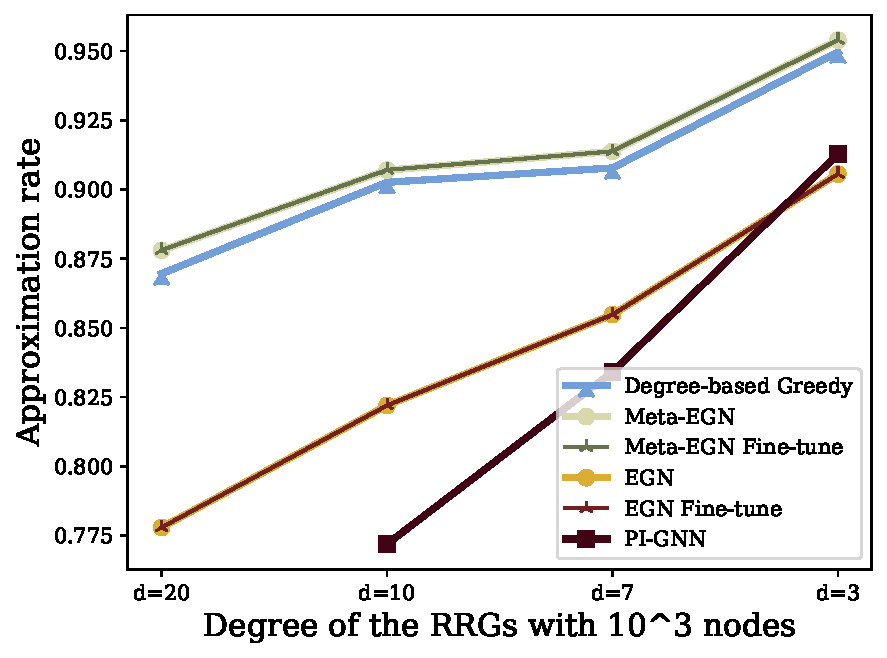
\includegraphics[width=0.32\textwidth]{iclr2023/img/intro/mis_10_3.pdf}
%         \vspace{-0.6cm}
      %   \caption{Performance with $10^3$ vertices}
       %  \label{fig:mis_103}
     %\end{subfigure}
     \hfill
     %\begin{subfigure}[c]{0.32\textwidth}
      %   \centering
         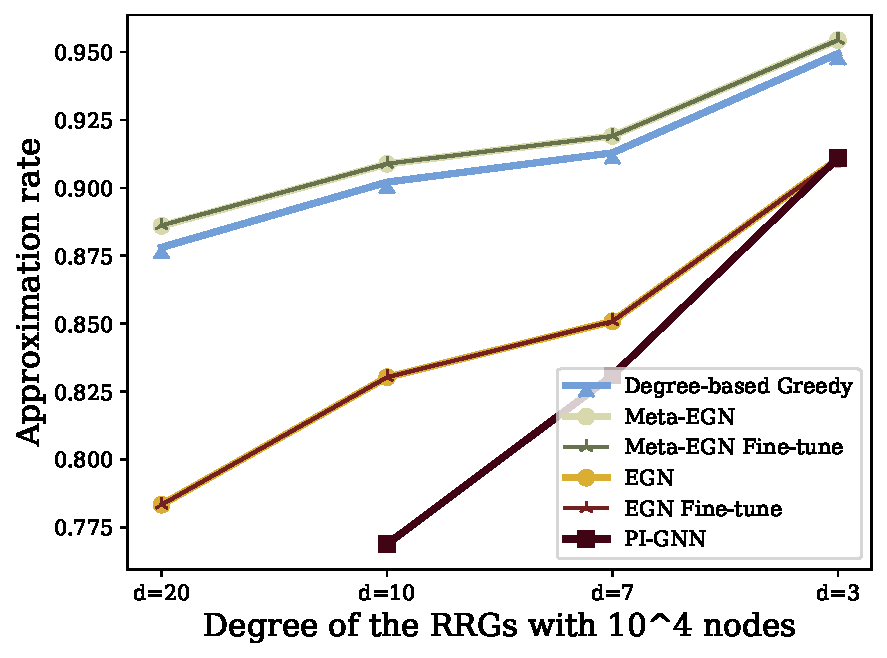
\includegraphics[width=0.32\textwidth]{iclr2023/img/intro/mis_10_4.pdf}
       %  \vspace{-0.6cm}
        % \caption{Performance with $10^4$ vertices}
        % \label{fig:mis_103}
     %\end{subfigure}
     \hfill
     %\begin{subfigure}[c]{0.32\textwidth}
      %   \centering
         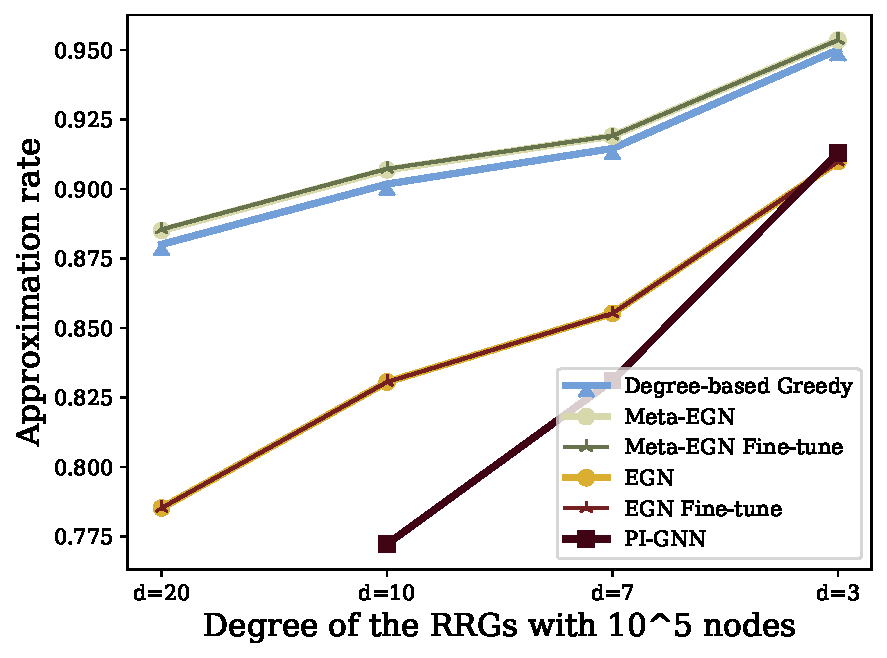
\includegraphics[width=0.32\textwidth]{iclr2023/img/intro/mis_10_5.pdf}
       %  \vspace{-0.6cm}
        % \caption{Performance with $10^5$ vertices}
         %\label{fig:mis_103}
    % \end{subfigure}
     \vspace{-0.3cm}
        \caption{Approximation Rates of different methods in the MIS problem.  \proj and EGN~\citep{karalias2020erdos} are trained on RRGs with $1000$ nodes and with node degree randomly sampled from $3,7,10,20$. \proj and EGN are evaluated over larger RRGs with $10^3\sim10^5$ nodes. More details about the setting are in Secs.~\ref{sec:settings} and~\ref{sec:MIS}. Meta-EGN outperforms DGA~\citep{angelini2019monte} by about $0.3\%-0.5\%$ in approximation rates on average.}
        \label{fig:mis}
        \vspace{-0.6cm}
        
\end{figure}

%instead of the per-instance optimality \pan{I think this statement is too technical.}. Note that the actual goal of CO is to find the optimal solution for each single instance encountered in the testing stage. There always exists a performance gap between the current optimization goal and the actual goal of CO, unless the model could learn an almost `one-to-one' mapping from the exponential input space to every optimal solution, which is currently impractical due to the limitation on the model's expressive power~\cite{chen2019learning,srinivasan2019equivalence,you2019position}, the training data volume~\citep{yehuda2020s} and the number of parameters \pan{This is so technical. Also, the previous references on expressive power are incorrect. The better way is to use practical example to claim in practice one-example instance is what is needed. Claim that generalization is importance.}. This gap seems passable in other ML applications such as computer vision or natural language  \pan{No one can understand this... This type of discussion should be put into the methodology part and pair it with an illustrative figure.}. These problems have less non-convex optimization landscapes, where different non-trivial local minima share similar values that are close to the global optimum~\citep{choromanska2015loss,kawaguchi2019every} \pan{Have you checked these references?}, which enables the networks to easily find out one in the expectation sense. Also, due to the regular and well-clustered feature map, once a good local optimum over expectation is achieved, the networks could easily grasp mapping patterns for interpolations on unseen data to obtain acceptable per-instance performance \pan{Do we need to claim per-instance performance of non-CO tasks? Per-instance performance cannot be pursued is because of objective is un-defined when without labels}. But as to CO, such gap could be significantly magnified. It's more difficult for CO problems to reach even the optimum over expectation. The non-convex optimization landscape of CO is intricate with high variance \pan{references?}, trapping the models in the non-trivial local optima without anymore guarantees on the distance from the global optimum \pan{Kind of over-claim because in traditional non-CO tasks, there is also no guarantee, also needed to be put into Method part}.  Also, interpolation on unseen data could be more easily spoiled \pan{interpolation?}. Instances in CO are more distinct from each other \pan{These descriptions are so subjective}, `similar' inputs with slight difference (i.e. adding/removing a single edge or vertex) might lead to entirely different solutions \pan{do you mean different optimal solutions? Can it be still a good approximate solution? Why I need optimal solution? Traditional ERM also does not guarantee optimal solution. The statement should be rephrased}. More aptly, each instance in CO appears to be an independent `task' rather than being as strongly connected with others as in common ML-based problems, which is naturally similar with the `few-shot learning' or even `zero-shot learning' setting \pan{This is not strong/certain enough. It is zero-shot learning problem. Also, the connection to zero shot should be proposed after the next paragraph.}.

%Thanks to unsupervised learning which makes gradient based fine-tuning on testing data a reality, An intuitive idea to curtail the gap is to train the objective on single instances. However, directly solving the per-instance optimality from scratch would not only be even more easier to trap the parameters into trivial local optima but also be less time-efficient \pan{Why?} than other CO solvers \pan{Do you assume the former is NN-based when saying this?}. To address the issues, we lend ourselves to a special formulation of machine learning, meta-learning specifically. We use the historical graphs to obtain a good initialization of the network parameters such that a limited-step (one-step in our case for comparable time-efficiency) fine-tune could make a leap towards the per-instance optimality \pan{Do you need to cite MAML?}. Also, aligned with the distinct characteristic of CO instances by regarding them as independent tasks, the meta method naturally ameliorates the models' generalization ability in the case, as displayed in Figure~\ref{intro:learning_curve} \pan{This figure does not show generalization. }. \pan{Two aspects of the benefits should be emphasized: Per-instance optimality \& generalization. I do not think these two aspects are properly explained and motivated.}

We demonstrate the benefits of \proj via experiments within three benchmark CO problems (max clique, vertex cover, and max independent set) on multiple synthetic graphs and three real-world graph datasets, with the number of nodes ranging from $100$ to $5000$. \proj significantly outperforms state-of-the-art learning-based baselines~\citep{karalias2020erdos,toenshoff2021graph}, greedy algorithms, and the commercial CO solver Gurobi9.5~\citep{Gurobi} in most cases. \proj also shows super OOD generalization performance when the training and test datasets are different or have graphs of entirely different sizes.   %significantly outperforms We also compare different methods over OOD graphs?}

%brought by our method in all the tasks over all the datasets, our framework also outperforms the previous state-of-the-art unsupervised frameworks~\citep{toenshoff2021graph} and the greedy algorithms. Our method also exceeds the current state-of-the-art commercial CO solver Gurobi9.5~\citep{Gurobi}, especially in large scale and hard instances. We do extensive experiments across the graph distribution (real-to-real, real-to-synthetic, synthetic-to-real, synthetic-to-complement) and across scales (from $500$ to $2000$) to further confirm our conjecture on our meta objective's ability in improving the generalization ability. Surprisingly, we also find our method could outperform the EGN even without the one-step fine-tuning, we attribute the phenomenon to meta's ability in finding out better local minima as initialization.


%We observe a significant boost in performance on EGN~\citep{karalias2020erdos} brought by our method in all the tasks over all the datasets, our framework also outperforms the previous state-of-the-art unsupervised frameworks~\citep{toenshoff2021graph} and the greedy algorithms. Our method also exceeds the current state-of-the-art commercial CO solver Gurobi9.5~\citep{Gurobi}, especially in large scale and hard instances. We do extensive experiments across the graph distribution (real-to-real, real-to-synthetic, synthetic-to-real, synthetic-to-complement) and across scales (from $500$ to $2000$) to further confirm our conjecture on our meta objective's ability in improving the generalization ability. Surprisingly, we also find our method could outperform the EGN even without the one-step fine-tuning, we attribute the phenomenon to meta's ability in finding out better local minima as initialization.

Moreover, recently, \cite{angelini2022cracking} have shown that the learning-based method in~\citep{schuetz2022combinatorial} could not achieve comparable results with the degree-based greedy algorithm (DGA)~\citep{angelini2019monte} in the max independent set (MIS) problem on large-scaled random-regular graphs (RRGs), which raises attentions from machine learning community. We observe the issues come from two aspects: (1) graph neural networks (GNNs) used to encode the regular graph suffer from the node ambiguity issue due to their limited expressive power~\citep{xu2018powerful}; (2) the model in~\citep{schuetz2022combinatorial} did not learn from history but was directly optimized over each testing case, which tends to be trapped into a local optimum. By addressing these two issues, \proj can consistently outperform DGA while maintaining the same time complexity to generate solutions. Fig.~\ref{fig:mis} show the results. %Meta-EGN and EGN are only trained on graphs with $10^3$ nodes and test on graphs with $10^3\sim10^5$ nodes.

%that our meta learning framework for CO could indeed learn heuristics from the greedy algorithms, which could achieve better performance, maintain the same time complexity and obtain good generalization ability across very large scales changes from $10^2$ to $10^5$, even before the fine-tuning step on testing data. The performance of our framework is shown in Figure~\ref{method:learning_curve}\hl{to be revised}.

%posed a big concern for ML for CO by

\iffalse
In addition, parameters of the models tend to be more conservative due to the `penalty' constraint in the training objective. Considering the penalty, a tiny change (i.e. setting one optimization variable from 0 to 1) on prediction might directly ruin the loss value. Thus rather than obtaining insignificant reward for better approximations for certain instances by taking the risk of breaking any constraint among the training data, the parameters prefer to guarantee feasible but not the best solution that it could reach for the whole data distribution, which would further widen the gap.


$\bullet$ Recent years have witnessed a boost in machine learning for combinatorial optimization. 
\pan{General motivation on learning for CO should be provided.}

formulation of problem (The goal of CO, in words not formulation), 
\begin{align*}
    \min_{X\in \Omega} f(X;D).
\end{align*}
introduce what methods could solve the problem (supervised in 1-2 sentences).

\pan{Do we need to slightly explain why we consider unsupervised learning?}
$\bullet$ Among the outstanding works, the Erd\H{o}s goes neural (EGN) introduces an unsupervised learning framework guided by the probabilistic methods. 

\pan{The following paragraph is too technical for intro. I suggest you first write Sec. 3 to make sure your notations/terminology are all comfortable in your mind. Then, write Sec. 1. Then, revise Sec. 3 according to Sec. 1. I still think there is some very basic intuition to motivate our formulation, which you do not need to directly intro ERM formulation.} \pan{For example ``Our idea comes from the simple first principle of the standard CO formulation: The goal of CO is to find the optimal solution for every instance encountered in the testing stage. However, previous works on unsupervised learning for CO \cite{EGN and others} always adopts an learning objective whose goal is to achieve optimality in the expectation sense over a certain distribution of instance, instead of optimality per instance, which yields suboptimal performance.''}\pan{Raise one/two real-world example.} But EGN formulates the training goal of the unsupervised learning for CO in an empirical risk minimization (ERM) form:  Suppose there a data distribution $D\sim P_{D}$ \pan{$\mathbb{P}_D$}. EGN aims to learn a parameterized randomized algorithm $P(X|D,\theta)$ to generate $X\in \Omega$ so as to minimize $E_{D\sim P_D}E_{X\sim P(X|D,\theta)}(f(X;D))$  \pan{$\mathbb{E}_D$}. That is
\begin{align*}
    \min_{\theta}E_{D\sim P_D}E_{X\sim P(X|D,\theta)}(f(X;D)).
\end{align*}
This goal aims for a good performance under the expectation considering the distribution of the testing dataset.

\pan{Define}
\begin{align*}
    l(\theta, D):\triangleq \mathbb{E}_{X\sim \mathcal{A}_{\theta}(D)}[f(X;D)] 
\end{align*}

\begin{align*}
     \textbf{Prev. Goal:} \min_{\theta}\mathbb{E}_D[l(\theta, D)]
\end{align*}

Actually, the goal is to do $\min_{\theta} l(\theta, D)$ for any $D\in \mathbb{P}_D$. 


\pan{However, directly solving $\min_{\theta} l(\theta, D)$ suffers from two issues 1) could easily be trapped into local OPT; (Cite non-convex landspace paper and claim the tendency to be in bad local optimal) 2) Take a lot of time to optimize. To address both issues, we lend ourselves to a special formulation of machine learning, meta learning specifically. We use the historical graphs to obtain a good initialization of $\theta$ such that a limited-step (one-step in our case) finetune of $\theta$ may make it good for each instance.}

%So, we propose .... Learning here essentially works for getting a good initialization for the downstream instance-wise optimization. We expect the initialization to be already very good. A limited-step (one-step in our case) finetune may make it even better.}

\pan{Define}
\begin{align*}
    \tilde{l}(\theta, D):\triangleq \mathbb{E}_{X\sim \mathcal{A}_{\theta_D}(D)}[f(X;D)], s.t., \theta_D=\theta - \nabla_{\theta} l(\theta, D) 
\end{align*}

\pan{Our goal:}
\begin{align*}
    \rightarrow \textbf{Our Goal:}\;\min_{\theta}\mathbb{E}_D[\tilde{l}(\theta, D)] 
\end{align*}


\pan{Define}
\begin{align*}
    \tilde{l}(\theta, D): \mathbb{E}_{X\sim \mathcal{A}_{\theta_D^*}(D)}[f(X;D)], s.t., \theta_D^*= \argmin \mathbb{E}_{X\sim \mathcal{A}_{\theta}(D)}[f(X;D)]\;\text{initialized by $\theta$}
\end{align*}

\pan{Our goal:}
\begin{align*}
    \rightarrow \textbf{Our Goal:}\;\min_{\theta}\mathbb{E}_D[\tilde{l}(\theta, D)] 
\end{align*}

% \pan{Define}
% \begin{align*}
%     \tilde{l}(\theta, D):\triangleq \mathbb{E}_{X\sim \mathcal{A}_{\theta-\nabla l(\theta, D) }(D)}[f(X;D)] \;\text{with initialization $\theta= \theta^{(0)}$}
% \end{align*}


% \begin{align*}
%     \textbf{Our Training:} \frac{1}{n}\sum_{i=1}^n \min_{\theta_i} l(\theta_i, \theta_i^{(0)}, D_i)
%     \,\text{where} \,\theta_i^{(0)} = \argmin_{\theta}  \frac{1}{n}\sum_{j=1,j\neq i}^n l(\theta, D_j) \\
%     \rightarrow \textbf{Our Goal:}\;\mathbb{E}_D[\min_{\theta}l(\theta, \theta^{(0)}, D)] ,\text{where} \,\theta^{(0)} = \argmin_{\theta}  \mathbb{E}_D[l(\theta, D_j)] \\
% \end{align*}
$\bullet$ 
Nevertheless, for CO problems, instead of aiming to get an expected minimized objective value on the whole testing set, a more reasonable goal is to achieve as high performance as possible on each single testing instance, which could be written as follows: 

\begin{align*}
   E_{D\sim P_D}  \min_{\theta} E_{X\sim P(X|D,\theta)}(f(X;D)).
\end{align*}

Also, in many difficult CO problems, The optimal solution to very similar configurations may be entirely different, which makes it very hard to find the pattern.
(Here we might take zero-shot learning problem for comparison).

To fulfill the goal above and formulate the problem in a more reasonable manner, we aim to learn a network to give a good initialization for CO problem, then on each testing instance, we fine-tune the initialization produced by the NN for better performance given a time budget which is comparable to the current prevailing methods. This naturally corresponds to the idea of meta-learning, which targets at training the fine-tuning potential of the model to achieve better performance after several further gradient steps on each testing instance, making it much closer to our goal.

\pan{Here, first claim the theoretical benefits: 1). Performance. 2) Generalization. Then say experiments verify such. Use one paragraph to say nature paper v.s. nature paper comments (large scale, time efficient).}

\pan{To the best of our knowledge, we are to first...}

$\bullet$ Experiment results have shown the great potential that meta could bring to EGN from the following aspects: 1) highly boosts in performance (one real task and synthetic based on RB model), outperforms the SOTA CO solver Gurobi9.5 in hard tasks 2) even better generalization ability between the real datasets and the synthetic datasets 3) guided by simple baselines, has the potential to outperform the simple baselines (MD-GA).
\fi

\vspace{-1mm}
\section{Related Work}
\vspace{-1mm}
%We aim to train networks towards the goal of optimality for every encountered instance as well as making use of heuristics from historical graphs, and thus we introduce meta learning to the unsupervised learning for CO framework. Related works of learning for CO and meta learning are discussed below.
In the following, we review two groups of works: unsupervised learning for CO and meta learning. %and its better model OOD generalization.  

%\pan{The biggest things are how to balance something you have introduced in other parts of the paper, and something presented here. Practical paper writing only has limited pages. So, often such tradeoff should be made.}

%kwon2020pomo,kwon2021matrix,delarue2020reinforcement,nandwani2021neural

%Most previous LCO approaches are based on RL~\cite{bello2016neural,chen2019learning,kwon2020pomo,kwon2021matrix,khalil2017learning,delarue2020reinforcement,wang2021bi,kool2018attention,nandwani2021neural} or supervised learning~\cite{khalil2016learning,gasse2019exact,yehuda2020s}, as these two frameworks do not hold any special requirements on the formulation of CO problems. However, they often suffer from the issues of training instability and subpar generalization. Previous works on unsupervised learning for CO have studied satisfaction problems~\cite{amizadeh2018learning,toenshoff2019run}. Applying these approaches to general CO problems requires problem reductions. Others have considered max-cut~\cite{yao2019experimental} and TSP problems~\cite{hudson2021graph}, while these works depend on carefully selected problem-specific objectives.

%\textbf{Learning for Combinatorial optimization:}
%Among the learning for CO methods, some guide neural networks by the optimal solutions~\citep{joshi2019efficient,hudson2021graph,selsam2018learning,wang2019learning,wang2020combinatorial}, the others train their models with the expert inference from traditional CO solvers~\citep{khalil2016learning,gasse2019exact,nair2020solving}. Yet the dependence on labels requires considerable time effort and may lead to poor generalization ability~\citep{joshi2020learning}. ~\cite{yehuda2020s} proves that having solutions for polynomial many CO problems only gives the labels of a subset of the settings for the original CO problem. If these labels are used for training, the obtained network may not be well generalized to the problem beyond the subset of the settings.
%RL approach is an alternative solution~\citep{mazyavkina2021reinforcement,bello2016neural,chen2019learning,khalil2017learning,yolcu2019learning}. Although RL gets rid of the dependence on labels, the high variance, higher time complexity and hard explorations are still concerns. 

Previous works on unsupervised learning for CO have studied max-cut~\citep{yao2019experimental} and TSP problems~\citep{hudson2021graph}, while these works depend on carefully selected problem-specific objectives. Some works have investigated satisfaction problems~\citep{amizadeh2018learning,toenshoff2019run}. Applying these approaches to general CO problems requires problem reductions. The works most relevant to us are \citep{karalias2020erdos}, \citep{wang2022unsupervised} and \citep{schuetz2022combinatorial}. \cite{karalias2020erdos} propose an unsupervised learning framework EGN for general CO problems based on the Erd\H{o}s' probabilistic method, which bonds the quality of the final solutions with probability. \cite{wang2022unsupervised} generalize EGN and prove that if the CO objective can be relaxed into an entry-wise concave form, a solution of good quality can be deterministically achieved. This further inspires the design of proxy objectives for CO problems that may not have closed-form objectives, such as those in circuit design. \cite{schuetz2022combinatorial} have recently extended EGN to large-scale max independent set problems on random-regular graphs.

%relaxation-and-rounding principle in the objective design

%satisfaction problems~\cite{amizadeh2018learning,toenshoff2019run}. Applying these approaches to general CO problems requires problem reductions. Others have considered max-cut~\cite{yao2019experimental} and TSP problems~\cite{hudson2021graph}, while these works depend on carefully selected problem-specific objectives. \cite{karalias2020erdos} and \cite{wang2022unsupervised} are most relevant to us. \cite{karalias2020erdos} propose an unsupervised learning framework EGN for general CO problems based on the Erd\H{o}s's probabilistic method, which could bond the model's performance with high probability once a satisfactory loss is obtained. \cite{wang2022unsupervised} further generalizes the theoretical analysis of EGN and proves that if the objective sati \emph{entry-wise concave} relaxation-and-rounding principle in the objective design

%Among works on unsupervised learning for CO,~\cite{yao2019experimental} relax the objective and trained GNNs for the max-cut problem, ~\cite{amizadeh2018learning} mimic RL to learn the solution structure for circuit SAT problem, ~\cite{toenshoff2021graph} train RNN for max-SAT problems by maximizing the probability of prediction. ~\cite{karalias2020erdos} propose an unsupervised learning framework for CO based on the Erd\H{o}s's probabilistic method, which could bond the model's performance with high probability once a satisfying loss is obtained. ~\cite{wang2022unsupervised} further generalize the framework to achieve performance guarantee via the \emph{entry-wise concave} relaxation-and-rounding principle in the objective design \pan{this sentence needs revision}. ~\cite{schuetz2022combinatorial} extend the framework to large scale max independent set problems on random-regular graphs. Nevertheless, unsupervised learning frameworks above adopt a learning objective whose goal is to obtain optimality in the expectation sense over a certain data distribution, instead of optimality for every single instance, therefore yielding a performance gap.
%To the best of our knowledge, we are the first to consider narrowing such gap.

%\textbf{Meta Learning:} 
Meta learning is proposed to learn hyper-parameters or initialization from historical tasks and achieve fast adaption to new tasks. ~\cite{finn2017model} propose model-agnostic meta learning (MAML), which aimed to obtain good parameter initialization and be accommodated to few-shot learning tasks with limited steps of fine-tuning. ~\cite{nichol2018first} accelerate MAML by adopting first-order approximation on the gradient estimation. ~\cite{rajeswaran2019meta} introduce implicit-MAML that adopts an objective with fine-tuning till the stationary points on new tasks. Implicit-MAML does not fit our case because we try to avoid long-time fine-tuning. ~\cite{hsu2018unsupervised} study unsupervised learning under the meta learning framework and focused exclusively on vision tasks. To the best of our knowledge, our work is the first one to apply meta learning to unsupervised learning for CO. %~\cite{jeong2020ood} brings the MAML framework to out of distribution detection vision tasks, ~\cite{conklin2021meta} utilizes meta learning in out-of-distribution natural language processing tasks, marking the success of meta learning in improving out-of-distribution generalization.

%Meta learning aims to learn how to learn. In other words, meta learning learns hyper-parameters or initialization from historical tasks to achieve fast adaption to new tasks as well as better out-of-distribution generalization ability. ~\cite{finn2017model} propose model-agnostic meta learning (MAML), which aims to obtain good parameter initialization and accommodate to unseen few-shot learning tasks with limited steps of fine-tuning. On one hand, MAML and its following works have achieved excellent performance in various fields thanks to the meta learning's ability of fast adaption to new tasks. \pan{The following sounds like a loosely related list. It is better to claim how they are related to us.} E.g. ~\cite{nichol2018first} perform first-order approximation on the gradient estimation of MAML for time-efficiency, ~\cite{rajeswaran2019meta} introduce implicit-MAML by changing the objective for the optimality after infinite fine-tuning steps on new tasks. ~\cite{hsu2018unsupervised} perform unsupervised learning under the meta learning framework to better learn the representations and achieve high performance in down-stream vision tasks. On the other hand, ~\cite{jeong2020ood} brings the MAML framework to out of distribution detection vision tasks, ~\cite{conklin2021meta} utilizes meta learning in out-of-distribution natural language processing tasks, marking the success of meta learning in improving out-of-distribution generalization.

%As to CO problem specifically, we find a concurrent work~\citep{manchanda2022generalization} which utilizes MAML to help improve the across distribution or scale generalization of the supervised learning and RL methods in routing problems \pan{do we even want to review? as it is published so close.}. But it still requires extra training data in testing distribution for adaption to the unseen testing task. To the best of our knowledge, we are the first to align the distinct characteristic of CO instances with the meta learning's advantage in fast adaption and out-of-distribution generalization \pan{this statement is not fully clear.}. We formulate each training instance as an independent task \pan{this is duplicated}, after obtaining the initialization from these historical instances, we no longer require any further training data on the unseen distribution but instead directly fine-tune the model thanks to our unsupervised learning structure.

\iffalse
Early meta learning works either learn black-box \pan{why emphasize black-box?} recurrent \pan{recurrent models are what they call?} models to make predictions on only a few examples from the new tasks~\citep{andrychowicz2016learning,chen2017learning,hochreiter2001learning,schmidhuber1993neural} or learn shared representations from different tasks \pan{do you mean multi task? Are shared representations the goal?}~\citep{snell2017prototypical,vinyals2016matching}. Since ~\cite{finn2017model} introduced the model-agnostic meta learning which aims to obtain good parameter initialization that could rapidly adapt to new tasks with limited steps of fine-tuning, MAML has been one of the most prevailing optimization-based meta learning tools to resolve few-shot learning problem \pan{the previous sentence is so long.}. MAML and its following works'~\citep{rajeswaran2019meta,nichol2018first,rothfuss2018promp} empirical success in few-shot learning also arises the researchers' interest in meta learning from the theoretical side. ~\cite{finn2017meta} proves the approximation ability of meta-guided deep learning \pan{review the theory of meta is kind of useless and out of the scope}. ~\cite{farid2021generalization,rothfuss2021pacoh,chen2021generalization,fallah2021generalization} focus on theoretically analyzing the generalization ability of MAML, while ~\cite{park2019meta,gonzalez2020improved,denevi2018learning} work to further improve MAML's generalization ability. ~\cite{wang2021fast,goldblum2020adversarially} investigate the stability of few shot learning against adversarial attacks and further improve it with the help of meta learning. 

\hl{no meta for RL here} \pan{Are you sure?}
~\cite{manchanda2022generalization} propose a concurrent work which utilizes meta-learning to help improve the generalization ability of supervised learning and RL methods in routing CO problems. \pan{Beyond SL and RL v.s. USL? Any other key differences? For example, SL formulation still follows ERM. We are the first to propose per-instance optimality. Can we claim this?}
In our unsupervised learning for CO case, we also find that MAML could further improve the performance as well as generalization ability across distribution or scales, we attribute the phenomenon to the reason that the meta objective could find the initialization of much better local optima among the intricate optimization landscape, which largely benefit the CO problems with very distinct instances.


$\bullet$ Before: supervised for CO: poor generalization ability, time-costly to collect data \pan{Remember Also cite a few core RL papers}

$\bullet$ then:Erd\H{o}s goes neural(EGN), unsupervised comparable results, but not a proper training goal 

~\cite{karalias2020erdos} introduces an unsupervised probabilistic method which is very likely to obtain good solutions once a low loss value is acquired, while ~\cite{wang2022unsupervised} generalizes the method into a 'relaxation and rounding' framework, which is guaranteed to achieve high performance under a low loss value with the proposed 'entry-wise concave' principle. 

\pan{Short. I suggest to discuss the principle observed in proxy-CO paper. }

$\bullet$ recently: nature (just an extension of Erd\H{o}s), arises the question from cracking: not that efficient and reliable as simple baselines.  \pan{Short; I suggest put intro.}

$\bullet$ We extend Erd\H{o}s and open it in the correct way, (nature is wrong in random regular graph) and address the question from cracking.  \pan{Short; I suggest put intro.}

\subsection{Meta learning}
$\bullet$ what is meta learning \pan{What tasks meta learning has been typically to solve? How are they related to our case}
\pan{Meta learning for RL. Please review. }
$\bullet$ MAML and its followers shows good performance

$\bullet$ Recent some questions raised by sharp-MAML, MAML with negative learning rate... poor generalization ability? \pan{I think we should not discuss this point here. This point should be put when we use exp to verify our generalization and explain why previous theory is not applied.}

$\bullet$ Surprisingly, in CO problems, we do not observe such poor generalization, by contrast, we found it could even further boost the performance as well as improve generalization. The reason could be: CO is essentially a zero-shot task \pan{Avoid using terminology to explain another terminology. Use intuition to explain}.
\fi

\vspace{-0.5mm}
\section{Preliminaries: Notations and Problem Formulation} \label{sec:prelim}
\vspace{-1mm}
%\subsection{Problem Formulation of Combinatorial Optimization (CO)}
\textbf{Combinatorial Optimization on Graphs.} We follow the settings considered in~\citep{karalias2020erdos,wang2022unsupervised,schuetz2022combinatorial} and study CO problems on graphs whose solutions can be represented as a subset of nodes of the input graph instance, although our method could be applied to a broader range of problems. Suppose $\mathcal{G}$ is the universe of graph instances. Let $G(V,E)\in \mathcal{G}$ denote a graph instance where $V=\{1,2,...,n\}$ is the node set and $E$ is the edge set. Let $X=(X_i)_{1\leq i \leq n} \in \{0,1\}^n$ denote the discrete optimization variables defined on $V$, where $X_i=1$ denotes that node $i$ is selected in the output node subset. A CO problem on $G$ consists of a cost function $f(\cdot;G):\{0,1\}^n \rightarrow \mathbb{R}_{\geq0}$ and a feasible set $\Omega\subseteq \{0,1\}^n$ that stands for the finite set of all feasible $X$'s, and asks to solve %Given a CO asks to solve 
\begin{equation}
\label{eq:def_CO}
\begin{aligned}
\min_{X\in \{0,1\}^n} f(X;G) \quad \quad \text{s.t.} \quad X \in \Omega
\end{aligned}
\end{equation}\vspace{-2mm}

%Let $\Omega$ stand for the finite set of all feasible $X$'s that satisfy the constraints of a problem. For example, in the max independent set problem, $\Omega$ contains all $X$'s where for any pair of adjacent nodes $i,j$, $X_i\neq 1$ or $X_j\neq 1$. 

%The primary goal of CO is, given any instance $G$ from instance space $\mathcal{G}$, to minimize a cost function $f(\cdot;G)$ by finding out the best assignment of $X$ from the feasible set $\Omega$:
%discrete optimization variables are binary variables defined on the nodes of graphs
%each entry of $X$ corresponds to whether a vertex is chosen in the independent set and
% \begin{equation}
% \label{method:def_CO}
% \begin{aligned}
% \min_{X\in \{0,1\}^n} f(X;G) \quad \quad \text{s.t.} \quad X \in \Omega
% \end{aligned}
% \end{equation}
\textbf{Unsupervised Learning for CO.} The Erd\"{o}s-Goes-Neural (EGN) framework of unsupervised learning for CO proposed in~\citep{karalias2020erdos} is reviewed as follows. Here, we use the notation system in a follow-up work~\citep{wang2022unsupervised} as it is more clear. Learning for CO problem is to learn an algorithm $\mathcal{A}_{\theta}(\cdot):\mathcal{G}\rightarrow \{0,1\}^n$ typically parameterized by an NN where $\theta$ denotes the parameters of the NN such that given a graph instance $G$, $X=\mathcal{A}_{\theta}(G)$ gives a solution of Eq.~\ref{eq:def_CO}. %feasible solution $X\in\Omega$ and minimizes $f(X;G)$. 
In practice, directly optimizing the parameters $\theta$ is hard in general. 

Therefore, we may consider a relaxed cost function $f_r(\cdot;G):[0,1]^n \rightarrow \mathbb{R}_{\geq0}$ where $f_r(X;G)=f(X;G)$ on any discrete points $X\in\{0,1\}^n$ and a relaxed constraint $g_r(\cdot;G):[0,1]^n \rightarrow \mathbb{R}_{\geq0}$ where $\{X\in\{0,1\}^n: g_r(X;G) = 0\}$ and $\{X\in\{0,1\}^n: g_r(X;G) \geq 1\}$ defines the feasible set $\Omega$ and the infeasible set $\Omega^c$ respectively. Also, suppose the NN in $\mathcal{A}_{\theta}$ can give soft solutions $\bar{X}\in[0,1]^n$. Then, we may train $\theta$ by minimizing a label-independent loss function:
\begin{equation}
\label{eq:relax}
\begin{aligned}
\min_{\theta}\; l(\theta;G) \triangleq f_r(\bar{X};G) + \beta g_r(\bar{X};G) , \quad \bar{X} = \mathcal{A}_{\theta}(G),\;\text{for some}\;\beta>0.
\end{aligned}
\end{equation}
The significant observation made by \citep{wang2022unsupervised}, which generalizes the argument in~\citep{karalias2020erdos}, is a type of performance guarantee on the condition that $f_r$ and $g_r$ are entry-wise concave, which is satisfied in all the cases studied in this work: If the loss that achieves $l(\theta;G)<\beta$ for some $\beta > \max_{X\in\{0,1\}^n} f(X;G)$, then the discrete solution $X$ obtained by rounding the soft solution $\bar{X}=\mathcal{A}_{\theta}(G)$ according to Def.~\ref{def:rounding} is feasible $X\in\Omega$ and of good quality $f(X;G) \leq l(\theta;G)$.
\begin{definition}[Rounding]
%\vspace{-0.3cm}
\label{def:rounding}
For a soft solution $\bar{X} \in [0,1]^n$ and an arbitrary order of the entries (w.l.o.g 1,2,...,n), fix all the other entries unchanged and round $\bar{X}_i$ into $0$ or $1$ as $X_i = \arg\min_{j=0,1} f_r(X_1,...,X_{i-1},j,\bar{X}_{i+1},...,\bar{X}_n)+\beta g_r(X_1,...,X_{i-1},j,\bar{X}_{i+1},...,\bar{X}_n)$, replace $\bar{X}_i$ with $X_i$ and repeat this operation until all the entries are discrete.
%\vspace{-0.2cm}
\end{definition}



\section{Meta learning for Erd\"{o}s Goes Neural (\proj)}
%\subsection{\proj}
The above performance guarantee lays the theoretical foundation for EGN. However, the following practical issue motivates us to incorporate meta learning into EGN.
%the unsupervised learning framework.

\subsection{Motivation: What needed is learning for instance-wise good solutions}
 It is often time-consuming to perform online optimization of $l(\theta;G)$ for each encountered instance $G$. This also mismatches the goal of learning, i.e., learning heuristics from history/data. Therefore, a  pipeline commonly adopted is as follows. Suppose there is a set of training instances $G_i$, $1\leq i\leq m$, IID sampled from a distribution $\mathbb{P}_{\mathcal{G}}$. We optimize $\theta$ by following 
\begin{equation}
\label{eq:previous_goal}
\begin{aligned}
\min_{\theta} \;\sum_{i=1}^m l(\theta;G_i),
\end{aligned}
\end{equation}
which is similar to empirical risk minimization (ERM) in standard supervised learning. When a test instance $G$ appears, we apply the learned $\mathcal{A}_{\theta}$ to get a soft solution and round it to the final solution.

This pipeline cannot guarantee the quality for this instance $G$. Even if the training instances $G_i$, $1\leq i\leq m$ are in a large quantity (so in-distribution generalization is not a problem), and even if the test instance $G$ also follows $\mathbb{P}_{\mathcal{G}}$, we may not guarantee a low $l(\theta;G)$ for one particular $G$ because ERM only guarantees a low averaged performance $\mathbb{E}_{G\sim\mathbb{P}_{\mathcal{G}}}[l(\theta;G)]$.  This issue may also violate the condition to have a performance guarantee as reviewed in Sec.~\ref{sec:prelim}, as it is instance-wise. Here, we highlight that in practice even the minimal averaged loss $\min_{\theta} \mathbb{E}_{G\sim\mathbb{P}_{\mathcal{G}}}[l(\theta;G)]$ is often strictly greater than averaged instance-wise minimal loss $\mathbb{E}_{G\sim\mathbb{P}_{\mathcal{G}}}[\min_{\theta} l(\theta;G)]$, because practical NNs are not expressive enough to remember the optimal solution to every instance.% due to the complex structure of a CO problem~\citep{}.     %may not be further applied. 

Unfortunately, many practical CO problems actually expect \emph{instance-wise good solutions}. This is because every instance in practice is crucial. A terrible solution for one instance may raise a security issue (e.g., the surveillance-camera allocation problem) or cause huge economic losses (e.g., the routing problem in a transportation system). With this observation, our work is to address the problem by studying \emph{unsupervised learning for instance-wise good solutions to CO problems}.

%: For each encountered test instance $G$, a solution $X$ of good quality is needed.

%Practical CO problems often expect \emph{instance-wise good solutions}: For each encountered test instance $G$, a solution $X$ of good quality is needed. This is because every instance in practice is crucial. A terrible solution for one instance may raise security issue (e.g., the surveillance-camera allocation problem) or cause huge economic losses (e.g., the routing problem in a transportation system). However,

%\pan{The following is something used before}

% In theory, by minimizing Eq.~\ref{eq:previous_goal}, if a test instance $G$ follows $\mathbb{P}_{\mathcal{G}}$, directly apply the learned $\mathcal{A}_{\theta}$ to $G$ may expect to have a low $l(\theta;G)$

% an empirical risk minimization (ERM)        

% \cite{karalias2020erdos,wang2022unsupervised}

% IID sampled from a distribution $\mathbb{P}_{\mathcal{G}}$

% Suppose the training instances $G_i$, $1\leq i\leq m$ are IID sampled from a distribution $\mathbb{P}_{\mathcal{G}}$,  \cite{karalias2020erdos,wang2022unsupervised} optimize $\theta$ by following an empirical risk minimization (ERM)
% \begin{equation}
% \label{eq:previous_goal}
% \begin{aligned}
% \min_{\theta} \;\sum_{i=1}^m l(\theta;G_i).
% \end{aligned}
% \end{equation}
% This framework expects that by optimizing Eq.~\ref{eq:previous_goal}, the NN $\mathcal{A}_{\theta}$ can learn heuristics to generate a soft solution $\bar{X}=\mathcal{A}_{\theta}(G)$ for graph instances $G\sim\mathbb{P}_{\mathcal{G}}$. 


% %Therefore, if the test instances $G_i$, 
% %$m+1\leq i\leq m+q$ follow the same d  


% One expects the NN to learn heuristics by training $\theta$ over $\Xi$. 

% Suppose the set of training instances $\Xi=\{G_1,G_2,...,G_m\}$,
% By assuming a distribution of graph instances $\mathbb{P}_{\mathcal{G}}$
% assumes that there is a distribution of graph instances $\mathbb{P}_$


% The framework asks to relax the original objective: The relaxed cost function $f_r(\cdot;G):[0,1]^n \rightarrow \mathbb{R}_{\geq0}$ where $f_r(X;G)=f(X;G)$ on any discrete points $$ 

% learn a parameterized algorithm $\mathcal{A}_{\theta}(\cdot):\mathcal{G}\rightarrow \{0,1\}^n$, which give
 
% %Here, we use the notation in~\cite{wang2022unsupervised}. EGN   The unsupervised learning for CO framework~\cite{wang2022unsupervised}

% The unsupervised learning for CO framework~\cite{wang2022unsupervised} could be summarized as training a parameterized algorithm $\mathcal{A}_{\theta}$ with the loss function below:
% \begin{equation}
% \label{method:previous_loss}
% \begin{aligned}
% l(\theta;G) \triangleq f(\bar{X};G) + \beta g(\bar{X};G) , \quad \bar{X} = \mathcal{A}_{\theta}(G)
% \end{aligned}
% \end{equation}, where $f$ is the cost function and $g$ represents the penalty constraints such that $\Omega \triangleq \{X\in\{0,1\}^n: g(X;G) = 0\}, \stcomp{\Omega} \triangleq \{X\in\{0,1\}^n: g(X;G) \geq 1\}$. $\theta$ denotes the parameters of the neural network,  $\bar{X} \in [0,1]^n$ denotes the vector embeddings relaxed to continuous space, $\beta > \max_{X\in \Omega} f(X;G)$ is the penalty coefficient hyper-parameter. Note that the probabilistic loss function of EGN~\citep{karalias2020erdos} could also be adapted into the same form as above. The optimization goal of the unsupervised learning framework, is to minimize the population-level loss function in the expectation sense over a certain data distribution $G \sim \mathbb{P}_G$ in space $\mathcal{G}$:
% \begin{equation}
% \label{method:previous_goal}
% \begin{aligned}
% \min_{\theta} \mathbb{E}_{G\sim \mathbb{P}_G} l(\theta;G).
% \end{aligned}
% \end{equation}
% When encountered a testing instance $G'$, once the loss value achieves $l(\theta;G')<\beta$, a feasible solution $X=R(\mathcal{A}_{\theta}(G'))$ with performance guarantee $f(X;G') \leq l(\theta;G')$ could be generated via the rounding process $R(\cdot)$ as shown in Def.~\ref{method:def_rounding} below.
% \begin{definition}[Rounding]
% \vspace{-0.3cm}
% \label{method:def_rounding}
% For a continuous embedding $\bar{X} \in [0,1]^n$ and an arbitrary order of the entries (w.l.o.g 1,2,...,n), fix all the other entries unchanged and round $\bar{X}_i$ into $0$ or $1$ as $X_i = \arg\min_{j=0,1} f(X_1,...,X_{i-1},j,\bar{X}_{i+1},...,\bar{X}_n)+\beta g(X_1,...,X_{i-1},j,\bar{X}_{i+1},...,\bar{X}_n)$, replace $\bar{X}_i$ with $X_i$ and repeat this operation until all the entries are discrete.
% \vspace{-0.2cm}
% \end{definition}

%\subsection{}
% However, even if the obtained algorithm $\mathcal{A}_{\theta}$ manages to minimize the objective $\min_{\theta} \mathbb{E}_{G\sim \mathbb{P}_G} l(\theta;G)$, there is still no guarantee that the rounded solution $X=R(\mathcal{A}_{\theta}(G))$ would achieve optimality for the actual objective of CO $\min_{X} f(X;G)$ given any unseen $G \in \mathcal{G}$, with $R(\cdot)$ denoting the rounding procedure. Because there always \pan{always sounds a little bit overemphasis. You just need to say they are different.} exists a gap between the optimality in the expectation sense in Eq.~\ref{method:previous_goal} and the optimality for a single instance in Eq.~\ref{method:def_CO}. Let $Tr(\mathbb{P}_G)$ \pan{Bad notation} denote the training dataset sampled from $\mathbb{P}_G$, only if neural networks could not only remember the optimal solution $\arg\min_{X}f(X;G)$ of every training instance $G \in Tr(\mathbb{P}_G)$ to its optimal solution $\arg\min_{X}f(X;G)$, but also perform totally correct generalization on any unseen data $G' \in \mathcal{G} \backslash Tr(\mathbb{P}_G)$, shall the gap be erased. This is practically unrealistic due to the limitation on the models' expressive power\hl{reference} and the dataset volume~\citep{yehuda2020s}. Thus in practice, the cost obtained by optimizing the objective over expectation should be always greater or equal to the optimal solution for a single instance:  
% \begin{equation}
% \label{method:eq_gap}
% \begin{aligned}
% \forall G \in \mathcal{G}, \quad f(R(\mathcal{A}_{\theta}(G));G) \geq f(\arg\min_X f(X;G);G)
% \end{aligned}
% \end{equation}

\subsection{Training towards instance-wise optimality via Meta Learning}

Our idea to address the problem is to regard the goal of learning from history as to search for good initialization for future instances rather than give direct solutions. Such good initialization can be quickly fine-tuned by further optimizing the model for each instance, which ultimately gives instance-wise good solutions. However, in practice, we do not have access to any future/test instances. So, can we just use historical/training instances to implement the above idea? Our strategy is to view each training instance $G_i$ as a pseudo-test instance to test and optimize the quality of initialization given by the model. Specifically, this strategy gives us an objective
\begin{equation}
\label{eq:infinite_step}
\begin{aligned}
\min_{\theta} \;\sum_{i=1}^m \tilde{l}_i(\theta), \quad \text{where}\; \tilde{l}_i(\theta) = \min_{\theta_i} l(\theta_i;G_i) \;\text{with $\theta_i=\theta$ as initialization.}
\end{aligned}
\end{equation}
Eq.~\ref{eq:infinite_step} has some abuse of notations. The minimum $\tilde{l}_i(\theta)$  depending on the initialization $\theta$ is because of the non-convex nature of  $\min_{\theta_i} l(\theta_i;G_i)$, where the initialization $\theta_i=\theta$ matters significantly. 

\begin{algorithm}[t]
\caption{Train \proj and Test \proj with/without Fine-tuning}
\label{method:alg_table}
\begin{algorithmic}[1]
\Require Training instances $\Xi=\{G_1,G_2,...,G_m\}$; Hyperparameters: $\alpha, \gamma$.
\State Randomly initialize $\theta^{(0)}$
\For{each randomly sampled mini-batch $B_j\subset \Xi$, $j=0,1,...,K-1$} \Comment{Training starts}
%\State Sample instances $G_i \sim \mathbb{P}_G$ 
%\For {$K$ steps}
%\ForAll{$G_i\in B_j$}
%\State Evaluate $\nabla_{\theta}l(\theta;G_i)$
\State For each $G_i\in B_j$, compute the adapted parameter: $\theta_i^{(j)} = \theta^{(j)} - \alpha \nabla_{\theta^{(j)}}l(\theta^{(j)};G_i)$
%\EndFor
\State Update: $\theta^{(j+1)} \gets \theta^{(j)} - \gamma \nabla_{\theta^{(j)}} \sum_{G_i \in B_j} l(\theta_i^{(j)};G_i)$
\EndFor \\
\Return $\theta\leftarrow \theta^{(K)}$
\Comment{Training ends}
%\EndWhile \Comment{Training ends}
\State For a given testing instance $G'$: \Comment{Testing starts}
\If {fine-tuning is allowed} 
\State Fine-tune the parameters: $\theta_{G'} \gets \theta - \alpha \nabla_{\theta} l(\theta; G')$ 
\State Use Def.~\ref{def:rounding} to round the relaxed solution given by $\mathcal{A}_{\theta_{G'}} (G')$ \Comment {With fine-tuning}
%\State Rounding for discrete solution 
\Else
\State Use Def.~\ref{def:rounding} to round the relaxed solution given by $\mathcal{A}_{\theta} (G')$ \Comment {Without fine-tuning}
%\State Rounding for discrete solution
\EndIf \Comment{Testing ends}
\end{algorithmic}
\end{algorithm}

\begin{figure}[t]
     \centering
     \vspace{-1mm}
     \begin{subfigure}[c]{0.32\textwidth}
         \centering
         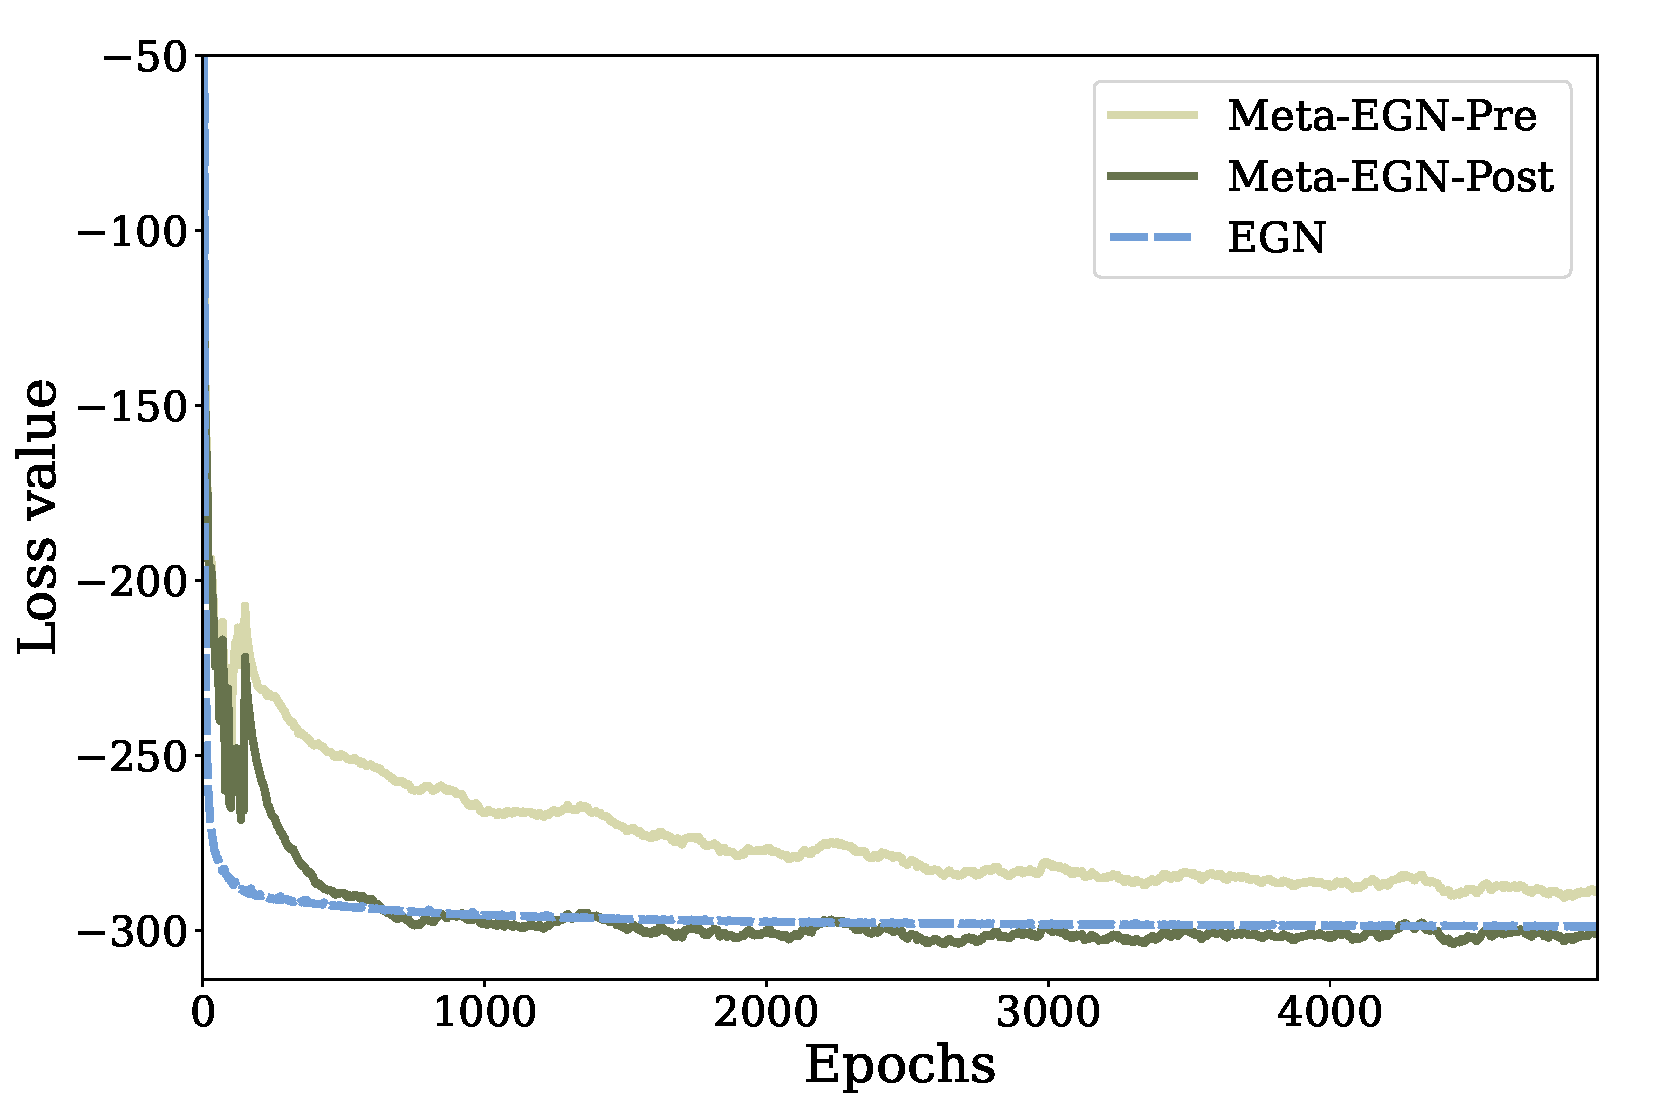
\includegraphics[width=\textwidth]{iclr2023/img/method/training_loss.pdf}
         \vspace{-0.6cm}
         \caption{Training Loss}
         \label{fig:dynamic_1}
     \end{subfigure}
     \hfill
     \begin{subfigure}[c]{0.32\textwidth}
         \centering
         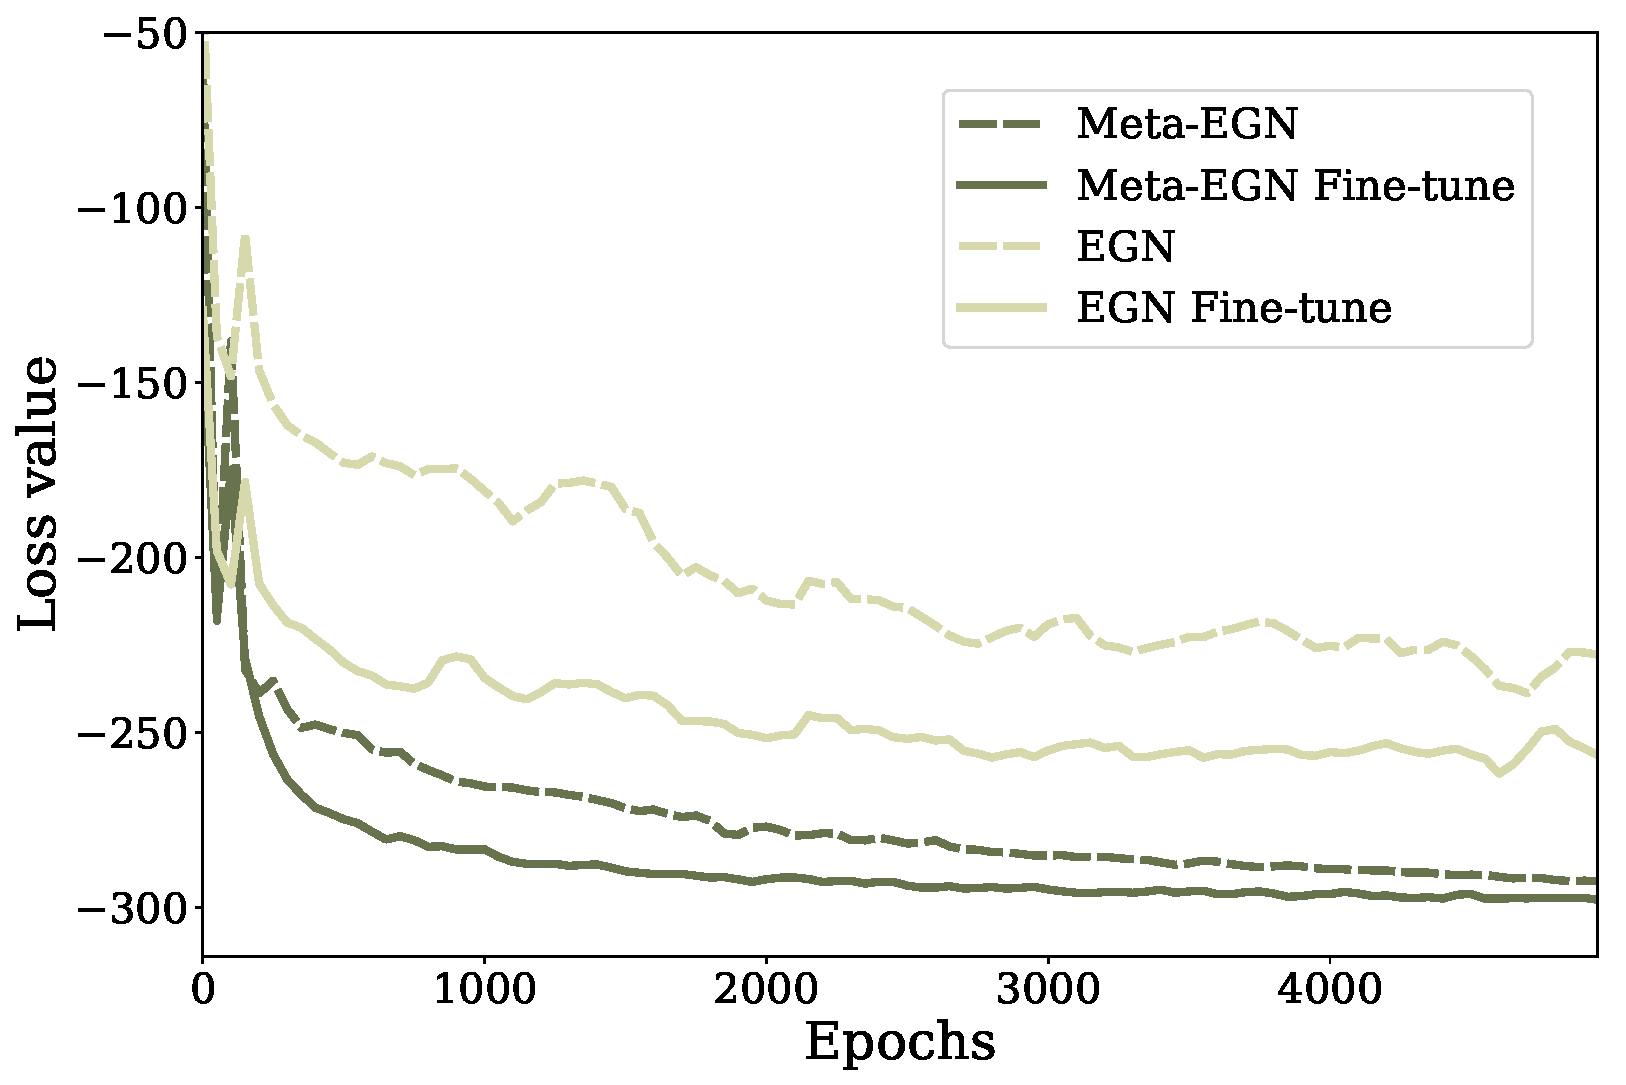
\includegraphics[width=\textwidth]{iclr2023/img/method/val_loss.pdf}
         \vspace{-0.6cm}
         \caption{Validation Loss}
         \label{method:fig_dynamic_2}
     \end{subfigure}
     \hfill
     \begin{subfigure}[c]{0.32\textwidth}
         \centering
         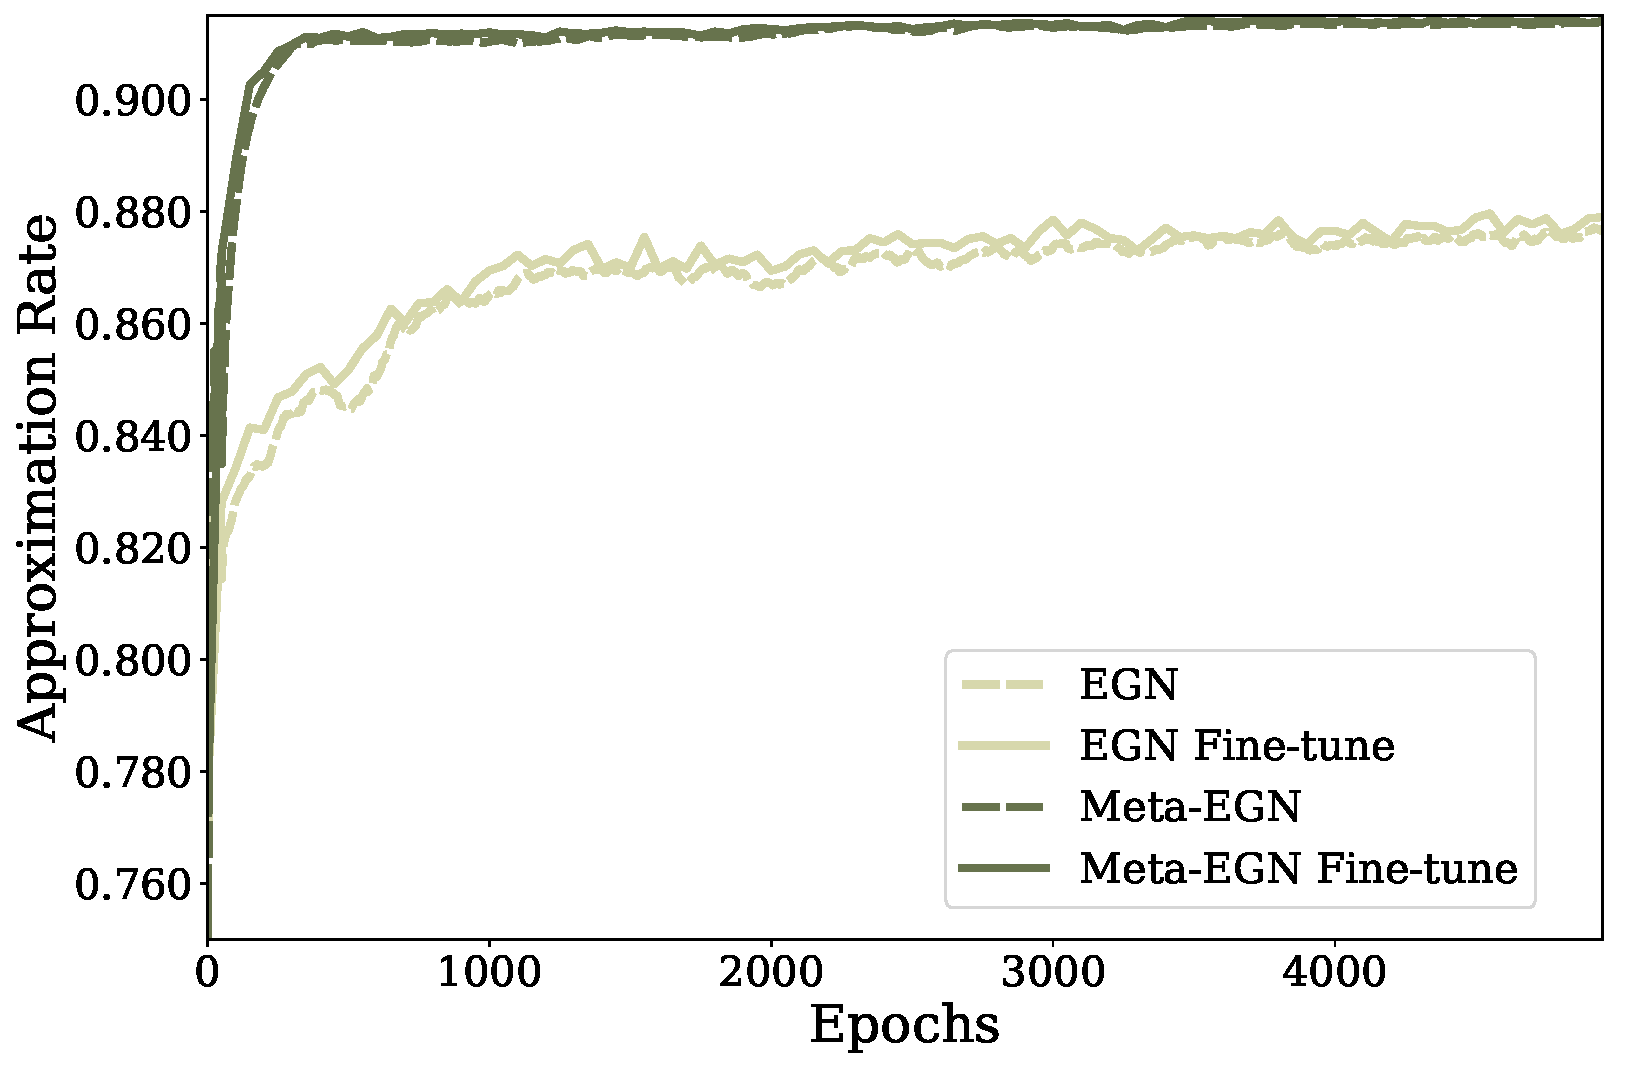
\includegraphics[width=\textwidth]{iclr2023/img/method/val_apr.pdf}
         \vspace{-0.6cm}
         \caption{Validation Approximation Rate }
         \label{fig:dynamic_3}
     \end{subfigure}
     \vspace{-0.2cm}
        \caption{Training/validating dynamics of \proj and EGN~\cite{karalias2020erdos} for the MIS problem.   Detailed experiment settings follow Sec.~\ref{sec:settings}.}
        \vspace{-0.2cm}%Other settings follow ~\citep{schuetz2022combinatorial,angelini2022cracking}.}  %In the training stage, the loss value of EGN framework is lower than that of \proj before the one-step inner gradient descent, but is higher than that of \proj after the one-step inner gradient descent. On validation set, a leap of the EGN losses of both before and after the fine-tuning could be observed, while the losses of \proj remain comparable to that during the training, revealing its higher generalization ability. Both the approximation rate (ApR) before and after fine-tuning of \proj on validation set outperforms EGN.}
        \label{fig:dynamic}
\end{figure}



We further simplify Eq.~\ref{eq:infinite_step} with some practical consideration. In fact, we may not allow further optimizing $\theta$ with so many gradient-descent steps for each instance, especially during the online test stage. As a proof of concept, we consider the case with only one-step gradient descent, which already gives good empirical results. Specifically, our training objective  follows
\begin{equation}
\label{eq:actual}
\begin{aligned}
\textbf{Our Objective:} \;\min_{\theta} \;\sum_{i=1}^m l_i(\theta), \quad \text{where}\; l_i(\theta) = l(\theta_i;G_i) \;\text{with $\theta_i=\theta -\alpha \nabla_\theta l(\theta;G_i)$.}
\end{aligned}
\end{equation}
Here, $\theta$ is to give a good initialization $\mathcal{A}_{\theta}(G_i)$ over each instance $G_i$ while $\theta_i$ is with one-step fine-tune to achieve a $G_i$-specified good solution $\mathcal{A}_{\theta_i}(G_i)$. 

Optimization in Eq.~\ref{eq:actual} can be implemented via the meta learning pipeline MAML~\citep{finn2017model}. We name the obtained model \proj and summarize its training and testing in Alg.~\ref{method:alg_table}. In step 3, \proj performs the one-step gradient descent on each training instance. Note that we consider two testing cases with or without fine-tuning because the latter saves much inference time. A simple extension of Theorem 1 in \citep{wang2022unsupervised} gives a performance guarantee for \proj in Theorem~\ref{thm:general_alpha} as follows. Here, for a test instance $G$, we even allow $l(\theta;G)$ to violate the original condition $l(\theta;G)<\beta$ in \citep{wang2022unsupervised} to some extent.  After one-step fine-tuning in step 9, the performance guarantee is still achievable. The detailed proof is in Appendix.~\ref{sec:proof-performance_guarantee}.% and the separated training/testing schedule is in Alg.~\ref{method:alg_table_train} and Alg.~\ref{method:alg_table_test} in the Appendix. %Interestingly, we observe that due to our training pipeline, \proj even without fine-tuning may 


\begin{theorem}[Performance Guarantee]
\label{thm:general_alpha}
Suppose the relaxations $f_r$ and $g_r$ are entry-wise concave as required in \citep{wang2022unsupervised}. Let $\theta$ denote the learned parameter after training.  Given a test instance $G$, suppose locally $l(\cdot;G)$ is $L$-smooth at $\theta$, i.e., $\|\nabla_{\theta'} l(\theta';G) - \nabla_{\theta} l(\theta;G)\|\leq L\|\theta' - \theta\|$ for all $\theta'$ that satisfies $\|\theta' - \theta\|\leq \epsilon$. Then, if \underline{$l(\theta;G) < \beta + \triangle$ (even if $l(\theta;G) \geq \beta$)}, for any $\alpha \in (0, 2/L)$ Meta-GNN with one-step finetuning outputs \underline{a feasible solution $X$ of good quality} $f(X;G)\leq l(\theta;G)-\triangle$. Here, $\triangle = \|\nabla_{\theta} l(\theta;G)\| \epsilon + \frac{1}{2L\alpha^2 - 4\alpha}\epsilon^2$ if $\epsilon < \alpha \|\nabla_{\theta} l(\theta;G)\|$ or $\triangle = (\alpha - \frac{L\alpha^2}{2})\|\nabla_{\theta}l(\theta;G)\|^2$ o.w..
\end{theorem}
%\begin{theorem}[Performance Guarantee]
%\label{thm:thm_performance_guarantee}
%Suppose the relaxations $f_r$ and $g_r$ are entry-wise concave as required in \citep{wang2022unsupervised}. Let $\theta$ denote the learned parameter after training.  Given a test instance $G$, suppose locally $l(\cdot;G)$ is $L$-smooth at $\theta$, i.e., $\|\nabla_{\theta'} l(\theta';G) - \nabla_{\theta} l(\theta;G)\|\leq L\|\theta' - \theta\|$ for all $\theta'$ that satisfies $\|\theta' - \theta\|\leq \epsilon$. Then, if \underline{$l(\theta;G) < \beta + \triangle$ (even if $l(\theta;G) \geq \beta$)}, there exists $\alpha$ such that Meta-GNN with one-step finetuning outputs \underline{a feasible solution $X$ of good quality} $f(X;G)\leq l(\theta;G)-\triangle$. Here, $\triangle = \|\nabla_{\theta} l(\theta;G)\|\epsilon - \frac{L}{2}\epsilon^2$ if $\epsilon< \frac{1}{L}\|\nabla_{\theta} l(\theta;G)\|$ or $\triangle=\frac{1}{2L}\|\nabla_{\theta} l(\theta;G)\|^2$ o.w..




% $<\beta$ 
% and $\theta_{G'}$ $\theta^*$ denote the corresponding local optimal parameter s.t. $\forall \theta \in \mathring{U}(\theta^*,\epsilon), l(\theta^*;G) < l(\theta;G)$, ($\mathring{U}(\cdot,\epsilon)$ is punctured neighborhood). Let $\beta > \max_{X \in \Omega} f(X;G)$ and $\min_{X\in \Omega}f(X;G)\geq 0$. Suppose the cost $f$ and constraint $g$ are entry-wise concave, $\theta$ achieves $l(\theta;G)<\beta$, and the inner fine-tune learning rate $\alpha \in (0,1/L_{\delta})$, where $L_{\delta}$ is the Lipschitz constant of the neighborhood $U(\theta;\delta)$ with a sufficiently small $\delta$,($\theta^*\notin U(\theta;\delta)$). Then with the fine-tuned parameter $\theta' = \theta - \alpha \nabla_{\theta} l(\theta;G)$, the relaxed solution $\bar{X} = \mathcal{A}_{\theta'}(G)$ generates a discrete solution $X \in \Omega$ such that $f(X;G) \leq l(\theta';G) \leq l(\theta;G)$ via the rounding process in Def.~\ref{def:rounding}.
%\vspace{-0.3cm}
%\end{theorem}



To better understand \proj, we show its training/testing dynamics in Fig.~\ref{fig:dynamic}. As we expected, the training loss of EGN is somewhere in-between the losses of \proj before and after the fine-tuning step. Training EGN is stabler and converges faster than training \proj. However, what is unexpected is that in validation, \proj has a much lower loss and achieves much better performance than EGN even before fine-tuning. 

This implies that \proj holds better generalization than EGN. We conjecture the reasons are as follows. First, the optimization landscape for CO problems is extremely non-convex~\citep{mezard2009information} due to the intersected feasible-infeasible regions and the high penalty coefficient $\beta$. 
EGN that has low losses for training instances may give a high loss even when the optimization landscape is just slightly shifted (from training to a test instance). However, the parameters of \proj are loosely tied to a local minimum for each training instance. Instead, those parameters, being aware of follow-up instance-wise fine-tuning steps, are likely to fall into some location close to a local minimum for each instance while being not trapped in any one of them, which makes the model robust to landscape shifts across instances. Second, a CO problem could vary a lot across graph instances even for those generated from the same distribution, especially when the instances are large. So, it is reasonable to view the problem over each instance as a separate but relevant task. %From this perspective, unsupervised learning for CO becomes a zero-shot learning task. 
Meta learning has shown good generalization when data distributions shift across tasks, which has empirical evidence in CV and NLP applications~\citep{jeong2020ood,conklin2021meta}.

%associates \proj with the capability of being adapted to the landscape shifts across instances. %See an illustration in Fig.~\ref{fig:landscape}.

As a summary, we provide a comparison between different unsupervised frameworks to solve CO problems in Table~\ref{tab:difference_methods}. Note that PI-GNN~\citep{schuetz2022combinatorial} is directly fine-tuned on each test instance without training so the fine-tuning time is long. Also, although PI-GNN also pursues instance-wise good solutions, its performance could be bad because it does not learn from training instances. The instance-wise solutions could be just bad local minima.  




% are easily trapped into valleys in the landscape with bad local minima. Having the per-instance gradient descent step during training, the model may understand better the lan 


% Slight perturbation on the parameters might substantially change the loss. 


% which leads to steep cliffs between the local minimum valleys, easily trapping the parameters in unsatisfactory ones. With the inner fine-tuning step, meta learning could potentially avoid the parameters from being trapped in bad local minima, leading to better performance and generalization.   


% in CO appears to be a more independent `task' rather than being as strongly connected with others as in common ML-based problems, which is similar with the `zero-shot learning' setting. Meta learning could naturally improve the out-of-distribution generalization~\citep{jeong2020ood,conklin2021meta} in few-shot learning tasks. 2) The optimization landscape of unsupervised learning for CO is much more intricate with high variance~\citep{mezard2009information} due to the scattered feasible-infeasible regions and the high penalty coefficient $\beta$. Any slight disturbance on the parameters might subvert the loss function, which leads to steep cliffs between the local minimum valleys, easily trapping the parameters in unsatisfactory ones. With the inner fine-tuning step, meta learning could potentially avoid the parameters from being trapped in bad local minima, leading to better performance and generalization. 3) During the training procedure, meta learning aims to guarantee the performance in the linear local regime before and after the inner fine-tune step, thus tending to choose the initialization inside deeper and better valleys, which results in better performance of the Mega-EGN over EGN even without the fine-tune step. Comparison between \proj with the other unsupervised methods is discussed in Tab.~\ref{method:tab_difference_methods}.


% However, what is 

% \proj boosts the performance of the previous framework EGN, as illustrated in the training dynamics of the max independent set problem on random-regular graphs in Fig.~\ref{method:fig_dynamic}. According to the training dynamics, the training loss of EGN is between those of \proj before and after its inner fine-tune step. Both the validation losses of EGN before and after fine-tune are much higher than those of \proj. Also, the validation approximation rate of \proj even with the learnt initialization still largely outperforms that of EGN either before or after the fine-tune. We attribute these observations to meta learning's ability in improving not only the performance but also the generalization ability. The reason behind such improvement could be summarized as follows: 1) Each instance in CO appears to be a more independent `task' rather than being as strongly connected with others as in common ML-based problems, which is similar with the `zero-shot learning' setting. Meta learning could naturally improve the out-of-distribution generalization~\citep{jeong2020ood,conklin2021meta} in few-shot learning tasks. 2) The optimization landscape of unsupervised learning for CO is much more intricate with high variance~\citep{mezard2009information} due to the scattered feasible-infeasible regions and the high penalty coefficient $\beta$. Any slight disturbance on the parameters might subvert the loss function, which leads to steep cliffs between the local minimum valleys, easily trapping the parameters in unsatisfactory ones. With the inner fine-tuning step, meta learning could potentially avoid the parameters from being trapped in bad local minima, leading to better performance and generalization. 3) During the training procedure, meta learning aims to guarantee the performance in the linear local regime before and after the inner fine-tune step, thus tending to choose the initialization inside deeper and better valleys, which results in better performance of the Mega-EGN over EGN even without the fine-tune step. Comparison between \proj with the other unsupervised methods is discussed in Tab.~\ref{method:tab_difference_methods}. 



%itself by regarding each training instance as an independent task as well as a pseudo-new task. Then whenever an unseen testing instance $G'$ is encountered, if some time for fine-tuning is allowed, one-step or even multiple steps (depending on the time limitation) fine-tuning is conducted on the testing instance to obtain the instance-particular parameter $\theta_{G'}$, aiming to move the initialization $\theta$ closer towards the per-instance optimality. $\theta_{G'}$ is then utilized to obtain $\bar{X} = \mathcal{A}_{\theta_{G'}}(G')$, followed by the rounding procedure in Def.~\ref{method:def_rounding} with performance guarantee (shown in Thm.~\ref{method:thm_performance_guarantee} below) to obtain the discrete solution $X$. If extreme rapid inference time is required, the initialization $\theta$ could be directly used to obtain the relaxed $\bar{X}$ and continue the same rounding. Note that although many of the traditional tasks (i.e. classification or regression) are also optimized for the optimality in the expectation sense, these tasks could not do anything better towards the optimality for single instances, because it is the unsupervised learning framework that gets rid of the labels and enables our one-step fine-tune on unseen testing instances to pursue optimality for a single instance. 




% Although this is not ideal, we expect that if test instances follow the same/similar distribution of training instances 

% draw on the heuristics from historical graphs to obtain a good initialization $\theta$ such that a limited step (one-step in our case considering time efficiency) fine-tuning of $\theta$ on the testing instance could further help the model leap closer to the per-instance optimality. The idea naturally aligns with the concept of meta learning, our loss function is thus defined as follows:
% \begin{equation}
% \label{method:meta_loss}
% \begin{aligned}
% \tilde{l}(\theta,G): \triangleq f(\bar{X};G)+\beta g(\bar{X};G), \quad \bar{X} = \mathcal{A}_{\theta_G}(G) \quad \text{s.t.} \quad \theta_G = \theta - \nabla_\theta l(\theta, G),
% \end{aligned}
% \end{equation}Our optimization objective could be summarized as:
% \begin{equation}
% \label{method:meta_goal}
% \begin{aligned}
% \min_{\theta} \mathbb{E}_{d \sim \mathbb{P}_G} \tilde{l}(\theta,G).
% \end{aligned}
% \end{equation}



% To narrow the gap above, our idea is to draw on the heuristics from historical graphs to obtain a good initialization $\theta$ such that a limited step (one-step in our case considering time efficiency) fine-tuning of $\theta$ on the testing instance could further help the model leap closer to the per-instance optimality. The idea naturally aligns with the concept of meta learning, our loss function is thus defined as follows:
% \begin{equation}
% \label{method:meta_loss}
% \begin{aligned}
% \tilde{l}(\theta,G): \triangleq f(\bar{X};G)+\beta g(\bar{X};G), \quad \bar{X} = \mathcal{A}_{\theta_G}(G) \quad \text{s.t.} \quad \theta_G = \theta - \nabla_\theta l(\theta, G),
% \end{aligned}
% \end{equation}Our optimization objective could be summarized as:
% \begin{equation}
% \label{method:meta_goal}
% \begin{aligned}
% \min_{\theta} \mathbb{E}_{d \sim \mathbb{P}_G} \tilde{l}(\theta,G).
% \end{aligned}
% \end{equation}

% With the training objective above, we train the unsupervised learning framework following the procedure as illustrated in Alg.~\ref{method:alg_table}: \proj performs meta learning with one step inner gradient descent on each training instance itself by regarding each training instance as an independent task as well as a pseudo-new task. Then whenever an unseen testing instance $G'$ is encountered, if some time for fine-tuning is allowed, one-step or even multiple steps (depending on the time limitation) fine-tuning is conducted on the testing instance to obtain the instance-particular parameter $\theta_{G'}$, aiming to move the initialization $\theta$ closer towards the per-instance optimality. $\theta_{G'}$ is then utilized to obtain $\bar{X} = \mathcal{A}_{\theta_{G'}}(G')$, followed by the rounding procedure in Def.~\ref{method:def_rounding} with performance guarantee (shown in Thm.~\ref{method:thm_performance_guarantee} below) to obtain the discrete solution $X$. If extreme rapid inference time is required, the initialization $\theta$ could be directly used to obtain the relaxed $\bar{X}$ and continue the same rounding. Note that although many of the traditional tasks (i.e. classification or regression) are also optimized for the optimality in the expectation sense, these tasks could not do anything better towards the optimality for single instances, because it is the unsupervised learning framework that gets rid of the labels and enables our one-step fine-tune on unseen testing instances to pursue optimality for a single instance. 



% \begin{theorem}[\proj's Performance Guarantee]
% \label{method:thm_performance_guarantee}
% Let $\theta$ denote the learnt initialization from training data, $\theta^*$ denote the corresponding local optimal parameter s.t. $\forall \theta \in \mathring{U}(\theta^*,\epsilon), l(\theta^*;G) < l(\theta;G)$, ($\mathring{U}(\cdot,\epsilon)$ is punctured neighborhood). Let $\beta > \max_{X \in \Omega} f(X;G)$ and $\min_{X\in \Omega}f(X;G)\geq 0$. Suppose the cost $f$ and constraint $g$ are entry-wise concave, $\theta$ achieves $l(\theta;G)<\beta$, and the inner fine-tune learning rate $\\alpha \in (0,1/L_{\delta})$, where $L_{\delta}$ is the Lipschitz constant of the neighborhood $U(\theta;\delta)$ with a sufficiently small $\delta$,($\theta^*\notin U(\theta;\delta)$). Then with the fine-tuned parameter $\theta' = \theta - \\alpha \nabla_{\theta} l(\theta;G)$, the relaxed solution $\bar{X} = \mathcal{A}_{\theta'}(G)$ generates a discrete solution $X \in \Omega$ such that $f(X;G) \leq l(\theta';G) \leq l(\theta;G)$ via the rounding process in Def.~\ref{def:rounding}.
% \vspace{-0.3cm}
% \end{theorem}

% \begin{algorithm}[h]
% \caption{\proj for CO}
% \label{method:alg_table}
% \begin{algorithmic}[1]
% \Require $\mathbb{P}_G$: distribution over the CO instances
% \Require $\alpha, \\alpha$: step size hyper-parameters
% \State randomly initialize $\theta$
% \While{not done} \Comment{Training starts}
% \State Sample instances $G_i \sim \mathbb{P}_G$ 
% %\For {$K$ steps}
% \ForAll{$G_i$}
% \State Evaluate $\nabla_{\theta}l(\theta;G_i)$
% \State Compute adapted parameters with gradient descent: $\theta' = \theta - \alpha \nabla_{\theta}l(\theta;G_i)$
% \EndFor
% \State Update: $\theta \gets \theta - \\alpha \nabla_{\theta} \sum_{G_i \sim \mathbb{P}_G} l(\theta';G_i)$
% %\EndFor
% \EndWhile \Comment{Training ends}
% \State For any given testing instance $G'$: \Comment{Testing starts}
% \If {fine-tune time is allowed}
% \State Fine-tune the parameters: $\theta_{G'} \gets \theta - \\alpha \nabla_{\theta} l(\theta; G')$ \Comment {Fine-tune for per-instance optimality}
% \State Inference the relaxed solution with fine-tuned parameters: $\bar{X} = \mathcal{A}_{\theta_{G'}} (\theta_{G'};G')$
% \State Rounding for discrete solution
% \Else
% \State Inference the relaxed solution directly: $\bar{X} = \mathcal{A}_{\theta} (\theta;G')$
% \State Rounding for discrete solution
% \EndIf \Comment{Testing ends}
% \end{algorithmic}
% \end{algorithm}

% \begin{figure}[t]
%      \centering
%      \begin{subfigure}[c]{0.32\textwidth}
%          \centering
%          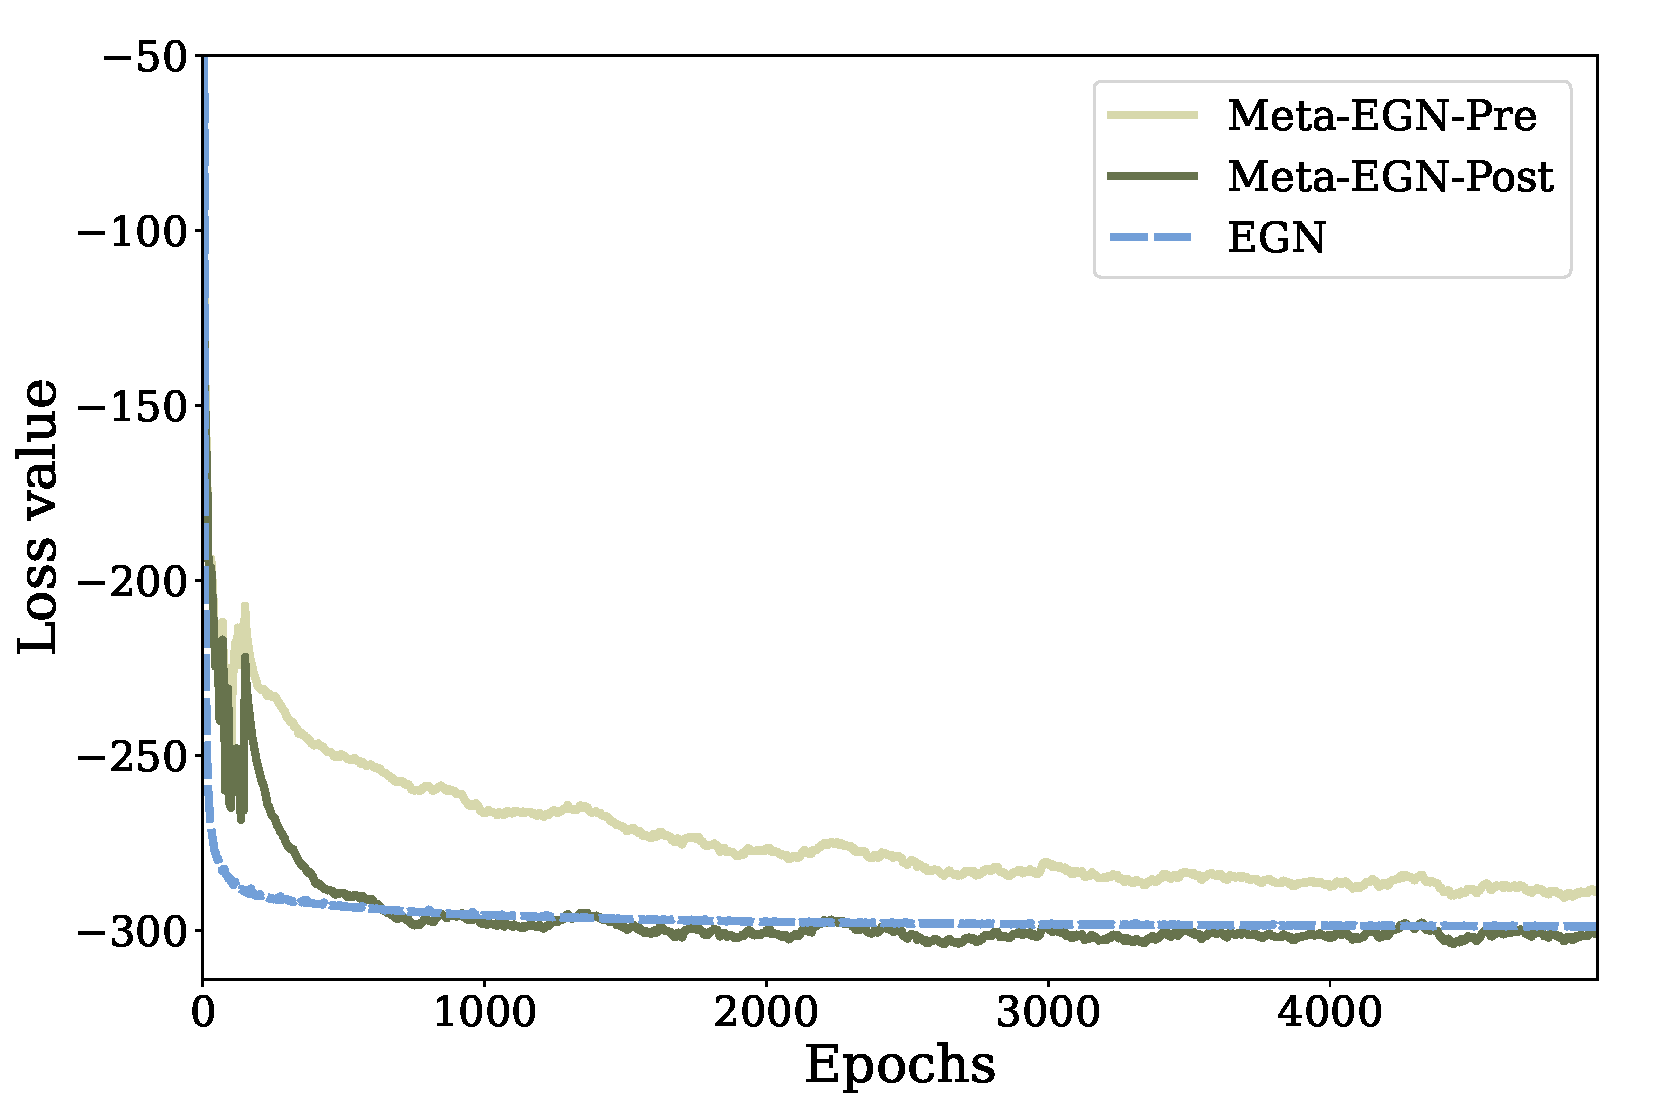
\includegraphics[width=\textwidth]{iclr2023/img/method/training_loss.pdf}
%          \vspace{-0.6cm}
%          \caption{Training Loss}
%          \label{method:fig_dynamic_1}
%      \end{subfigure}
%      \hfill
%      \begin{subfigure}[c]{0.32\textwidth}
%          \centering
%          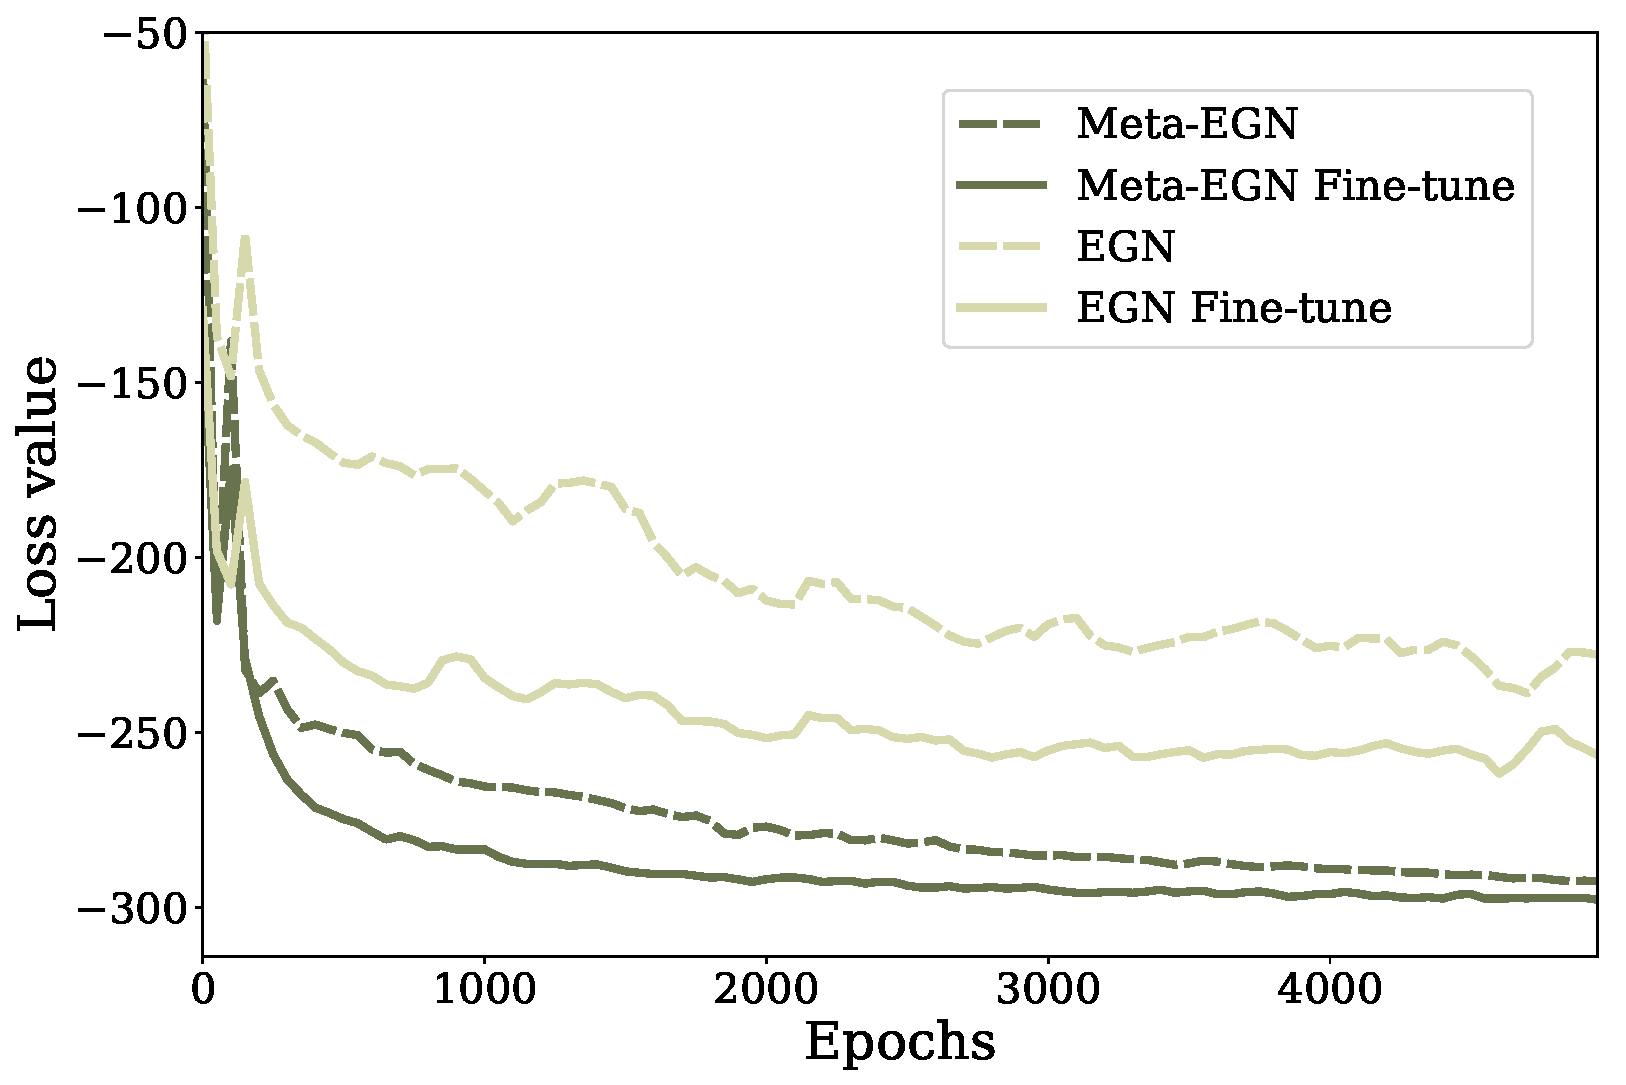
\includegraphics[width=\textwidth]{iclr2023/img/method/val_loss.pdf}
%          \vspace{-0.6cm}
%          \caption{Validation Loss}
%          \label{method:fig_dynamic_2}
%      \end{subfigure}
%      \hfill
%      \begin{subfigure}[c]{0.32\textwidth}
%          \centering
%          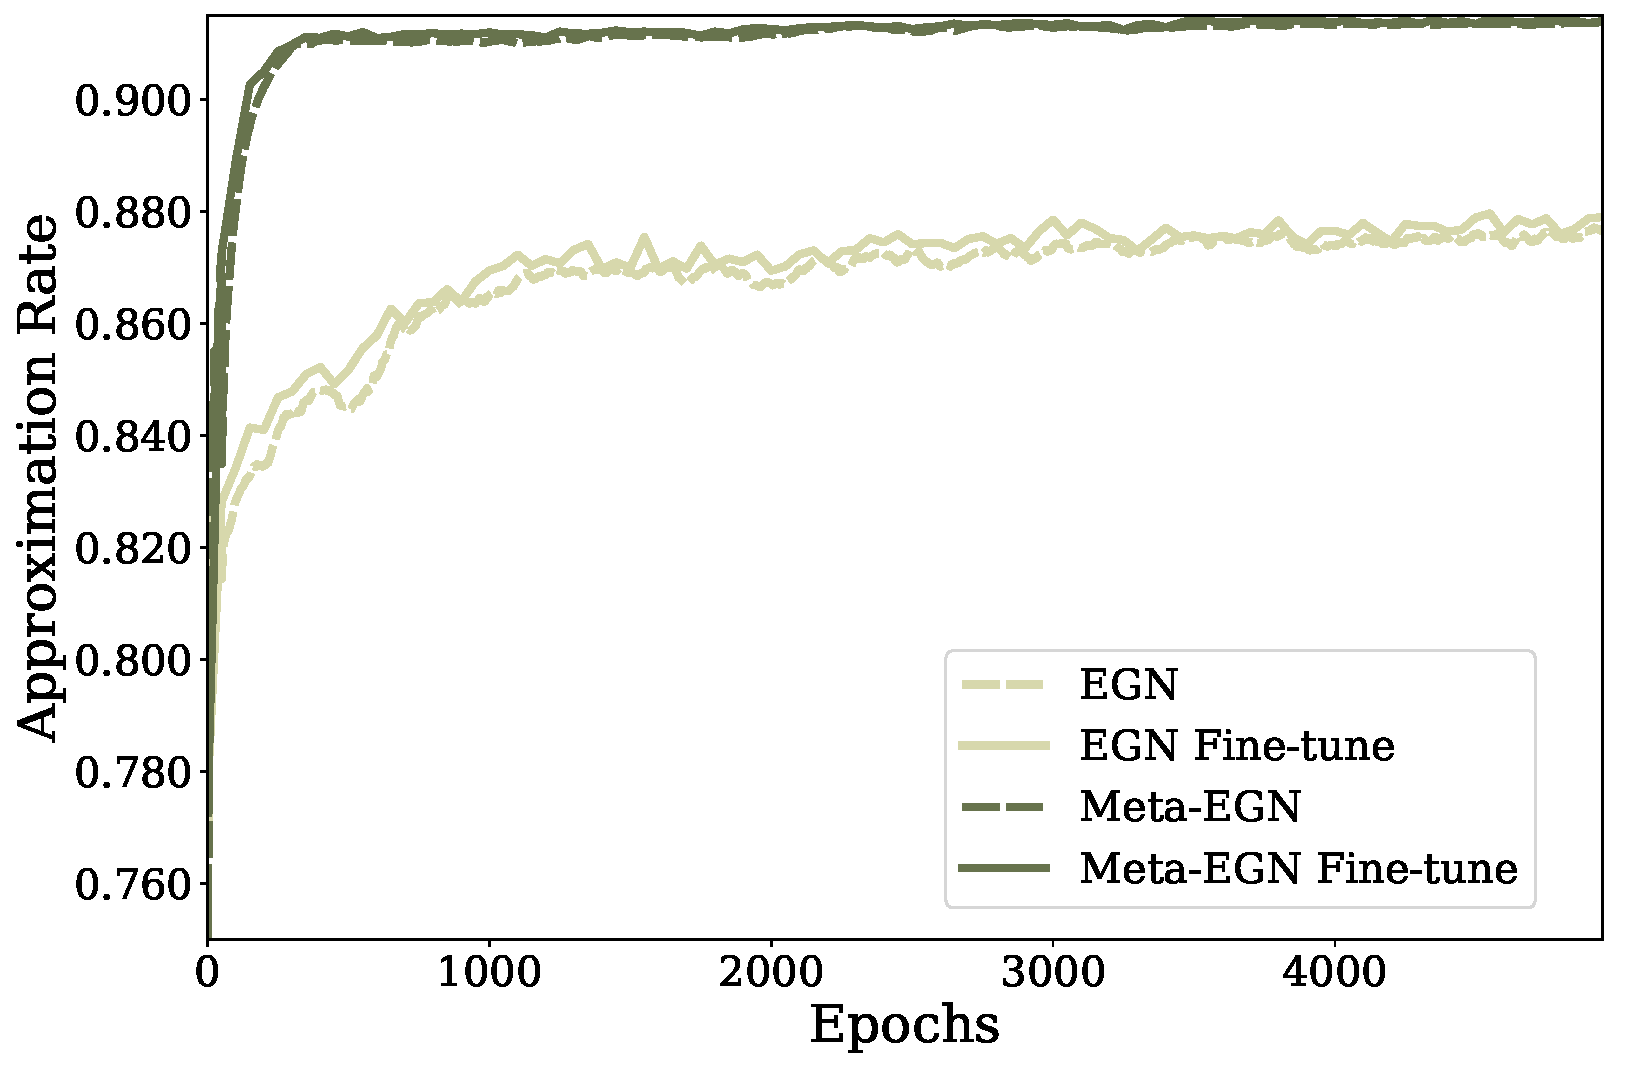
\includegraphics[width=\textwidth]{iclr2023/img/method/val_apr.pdf}
%          \vspace{-0.6cm}
%          \caption{Validation Approximation Rate}
%          \label{method:fig_dynamic_3}
%      \end{subfigure}
%      \vspace{-0.3cm}
%         \caption{Training dynamics of max independent set problem with mixed degrees $(3,5,7,10,20)$ on random-regular graphs with $1000$ vertices, where the settings follow ~\cite{schuetz2022combinatorial,angelini2022cracking}. In the training stage, the loss value of EGN framework is lower than that of \proj before the one-step inner gradient descent, but is higher than that of \proj after the one-step inner gradient descent. On validation set, a leap of the EGN losses of both before and after the fine-tuning could be observed, while the losses of \proj remain comparable to that during the training, revealing its higher generalization ability. Both the approximation rate (ApR) before and after fine-tuning of \proj on validation set outperforms EGN.}
%         \label{method:fig_dynamic}
% \end{figure}

% \proj boosts the performance of the previous framework EGN, as illustrated in the training dynamics of the max independent set problem on random-regular graphs in Fig.~\ref{method:fig_dynamic}. According to the training dynamics, the training loss of EGN is between those of \proj before and after its inner fine-tune step. Both the validation losses of EGN before and after fine-tune are much higher than those of \proj. Also, the validation approximation rate of \proj even with the learnt initialization still largely outperforms that of EGN either before or after the fine-tune. We attribute these observations to meta learning's ability in improving not only the performance but also the generalization ability. The reason behind such improvement could be summarized as follows: 1) Each instance in CO appears to be a more independent `task' rather than being as strongly connected with others as in common ML-based problems, which is similar with the `zero-shot learning' setting. Meta learning could naturally improve the out-of-distribution generalization~\citep{jeong2020ood,conklin2021meta} in few-shot learning tasks. 2) The optimization landscape of unsupervised learning for CO is much more intricate with high variance~\citep{mezard2009information} due to the scattered feasible-infeasible regions and the high penalty coefficient $\beta$. Any slight disturbance on the parameters might subvert the loss function, which leads to steep cliffs between the local minimum valleys, easily trapping the parameters in unsatisfactory ones. With the inner fine-tuning step, meta learning could potentially avoid the parameters from being trapped in bad local minima, leading to better performance and generalization. 3) During the training procedure, meta learning aims to guarantee the performance in the linear local regime before and after the inner fine-tune step, thus tending to choose the initialization inside deeper and better valleys, which results in better performance of the Mega-EGN over EGN even without the fine-tune step. Comparison between \proj with the other unsupervised methods is discussed in Tab.~\ref{method:tab_difference_methods}. 

% \begin{table}[h]
% \setlength\tabcolsep{1pt}
% \centering
% \footnotesize
% \begin{tabular}{@{}ccccc@{}}
% \toprule
%  &
%   \begin{tabular}[c]{@{}c@{}}EGN\\ ~\citep{karalias2020erdos}\end{tabular} &\begin{tabular}[c]{@{}c@{}}P-I GNN\\ ~\citep{schuetz2022combinatorial}\end{tabular}
%   &
%   \begin{tabular}[c]{@{}c@{}}\proj\\ (Ours)\end{tabular} &
%   \begin{tabular}[c]{@{}c@{}}Classical Solver\\ ~\cite{Gurobi} \end{tabular} \\ \midrule
% Goal           &     $\mathbb{E}_{D\sim \mathbb{P}_D} l(\theta;D)$     &   $l(\theta;D)$   &    $\mathbb{E}_{D\sim \mathbb{P}_D} \tilde{l}(\theta;D)$    &   $f(X;D) \  \text{s.t.} \  X \in \Omega$   \\
% Training  & Yes        &   No   & Yes & No   \\
% Fine-tune time & No & Very long   & Short  & Long \\
% Generalization &  Good        & - & Better & -    \\ \bottomrule
% \end{tabular}
% \caption{Comparison between our framework and the previous unsupervised frameworks.}
% \label{method:tab_difference_methods}
% \end{table}

\begin{table}[t]
\setlength\tabcolsep{1pt}
\centering
%\footnotesize
\caption{Comparison between different unsupervised frameworks. $G$ denotes the test instance and $G_i$, $1\leq i\leq m$ are training instances. The standard EGN pipeline does not adopt any fine-tuning.}
\label{tab:difference_methods}
\vspace{-3mm}
\resizebox{1\textwidth}{!}{
\begin{tabular}{@{}ccccc@{}}
\toprule
 &
  \begin{tabular}[c]{@{}c@{}}EGN\\ ~\citep{karalias2020erdos}\end{tabular} &\begin{tabular}[c]{@{}c@{}}P-I GNN\\ ~\citep{schuetz2022combinatorial}\end{tabular}
   &
  \begin{tabular}[c]{@{}c@{}}\proj\\ (Ours)\end{tabular} &
  \begin{tabular}[c]{@{}c@{}}Classical Solver\\ ~\cite{Gurobi} \end{tabular} \\ \midrule
Obj. to optimize the NN           &     $\sum_{i=1}^m l(\theta;G_i)$     &   $l(\theta;G)$   &    $\sum_{i=1}^m l(\theta -\nabla_{\theta} l(\theta;G_i) ;G_i)$    &   $f(X;G) \  \text{s.t.} \  X \in \Omega$   \\
Training or not  & Yes        &   No   & Yes & No   \\
Fine-tune timing & No & Long   & Short/No  &  Long  \\
Generalization &  Good        & - & Better & -    \\ \bottomrule
\end{tabular}}
\vspace{-1mm}
\end{table}

\vspace{-0.1cm}
\section{Experiments}\label{sec:exp}
\vspace{-0.1cm}
%\subsection{Case Study}
\begin{figure}
\begin{minipage}{0.63\textwidth}
%\begin{wraptable}{r}{0.5\textwidth}
%\begin{table}[t]
%\fontsize{10}{6}\selectfont
%\setlength\tabcolsep{4pt}
\centering
\captionof{table}{The discrete objectives (Eq.~\ref{eq:def_CO}) and their relaxations (Eq.~\ref{eq:relax}) for the three problems to be studied.}
\label{exp:tab_case_study}
\resizebox{\textwidth}{!}{\begin{tabular}{@{}ccc@{}}
\toprule
\multirow{2.5}{*}{MC} & Discrete Obj. & $\max_{X}  \sum_{1\leq i\leq n} X_i  \quad \quad \text{s.t.} \quad  (i, j) \in E\;\text{if}\;{X_i, X_j = 1} $ \\ \cmidrule(l){2-3} 

 & Relaxation & $l_{\text{MC}}(\theta;G) \triangleq - (\beta+1)\sum_{(i,j)\in E} \bar{X}_i \bar{X}_j + \frac{\beta}{2} \sum_{i \neq j} \bar{X}_i \bar{X}_j$ \\ \midrule
 
\multirow{2.5}{*}{MVC} & Discrete Obj. & $\min_{X} \sum_{1 \leq i \leq n} X_i \quad \quad \text{s.t.} \quad  X_i + X_j \geq 1\;\;\text{if}\;(i,j)\in E \ $ \\ \cmidrule(l){2-3} 

 & Relaxation & $l_{\text{MVC}}(\theta;G) \triangleq \sum_{1\leq i \leq n} \bar{X}_i +\beta \sum_{(i,j) \in E} (1-\bar{X}_i) (1-\bar{X}_j)$ \\ \midrule
 
% \multirow{2.5}{*}{MDS} & Formulation & $\min_{X} \sum_{1 \leq i \leq n} X_i \quad \quad \text{s.t.} \quad  \  (1-X_i) \prod_{j \in \mathcal{N}(i)} (1-X_j) \leq 0$ \;\text{if}\; $i \in V$\\ \cmidrule(l){2-3}

%  & Loss Design & $l_{\text{MDS}}(\theta;G) \triangleq \sum_{1 \leq i \leq n} \bar{X}_i + \beta \sum_{i\in V} (1-\bar{X}_i)\prod_{j \in \mathcal{N}(i)}(1-\bar{X}_j)$ \\ \midrule
 
\multirow{2.5}{*}{MIS} & Discrete Obj. & $\max_{X} \sum_{1 \leq i \leq n} X_i \quad \quad \text{s.t.} \quad  X_iX_j = 0 \;\text{if}\; (i,j) \in E$ \\ \cmidrule(l){2-3} 

 & Relaxation & $l_{\text{MIS}}(\theta;G) \triangleq -\sum_{1 \leq i \leq n} \bar{X}_i + \beta \sum_{(i,j) \in E} \bar{X_i} \bar{X_j}$ \\ \bottomrule
\end{tabular}}
%\end{wraptable}
%\end{table}
\end{minipage}
\hfill
\begin{minipage}{0.34\textwidth}
%\begin{figure}
%\begin{center}
\caption{Performance v.s. hyper-parameter $\rho$ of the RB model}
\vspace{-0.1cm}
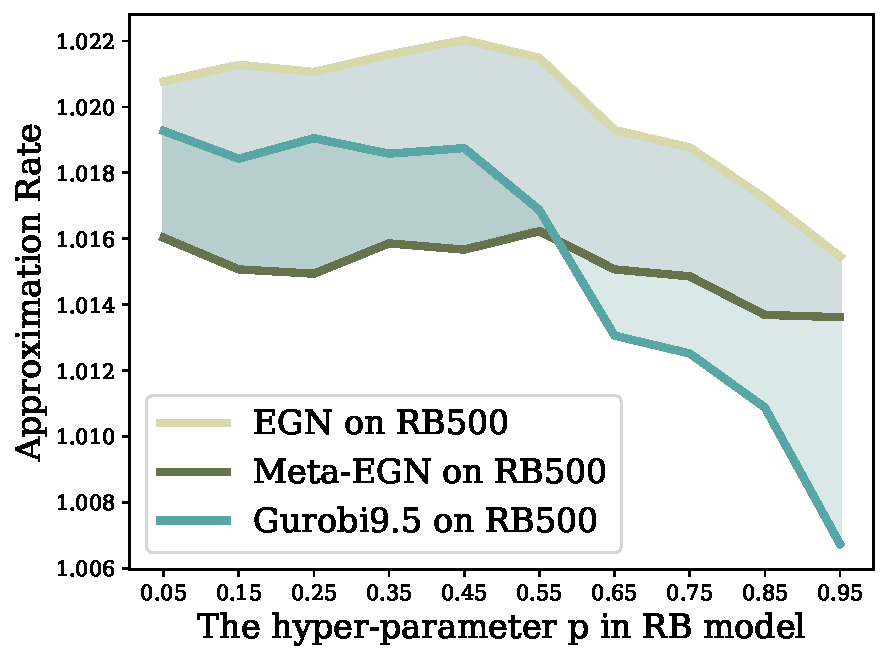
\includegraphics[width=0.92\textwidth]{iclr2023/img/exp/difficulty_mvc.pdf}
%\end{center}
\vspace{-0.5cm}
\label{fig:difficulty_rb}
%\end{figure}
\end{minipage}
\end{figure}

We study three CO problems, namely \emph{max clique (MC)} to find the largest set of nodes where each pair of nodes are connected,  \emph{minimum vertex covering (MVC)} to find the smallest set of nodes that every edge is connected to at least one nodes in the set, and  \emph{max independent set (MIS)} to find the largest set where any two vertices in the set are not adjacent. Their objectives (Eq.~\ref{eq:def_CO}) and relaxations (Eq.~\ref{eq:relax})  are listed in Table~\ref{exp:tab_case_study}. For the detailed derivation, see Appendix ~\ref{sec:app_experiment_details}.

%Also, if learning-based methods are fine-tuned based on the test instance, we highlight them with ``f-t''. We only consider

%\end{table}



\vspace{-0.1cm}
\subsection{Settings}\label{sec:settings}
\vspace{-0.1cm}
% \begin{wrapfigure}{r}{0.42\textwidth}
% \vspace{-1cm}
%   \begin{center}
%     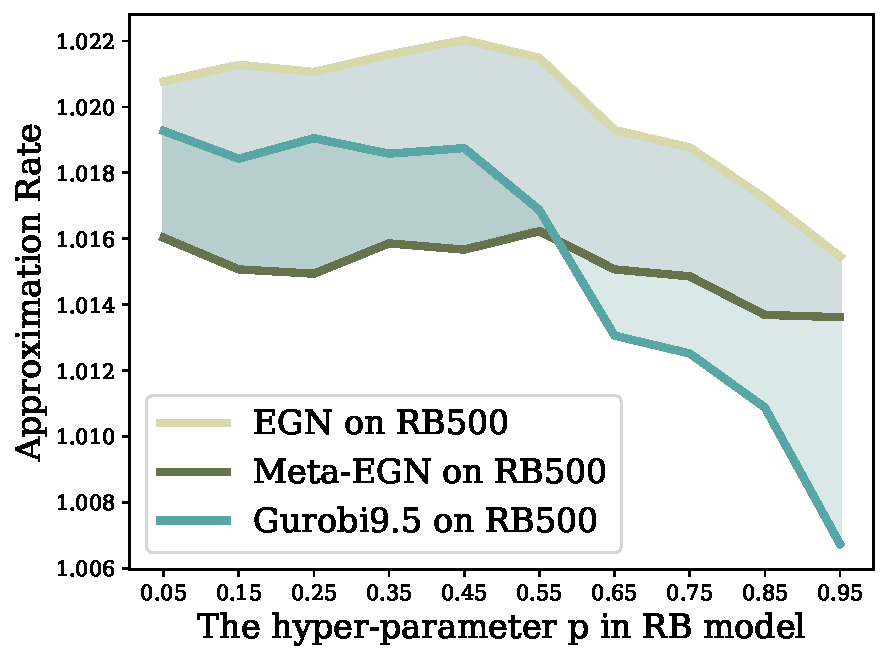
\includegraphics[width=0.42\textwidth]{iclr2023/img/exp/difficulty_mvc.pdf}
%   \end{center}
%   \vspace{-0.5cm}
%   \caption{Cross-Difficulty of RB on MVC}
%   \label{fig:difficulty_rb}
% \end{wrapfigure}

\textbf{Datasets:} We conduct experiments on the MC and MVC problems over three real datasets Twitter~\citep{leskovec2014snap}, COLLAB and IMDB~\citep{yanardag2015deep} and two synthetic datasets with $200$ and $500$ nodes generated by the RB model~\citep{xu2007benchmarks}. We name them RB200 and RB500, respectively. We make RB200 and RB500 extremely hard by setting a small hyper-parameter $\rho=0.25$ of the RB model~\citep{xu2007benchmarks}. The difficulty-$\rho$ relationship on the MVC problem with $500$ vertices is shown in Fig.~\ref{fig:difficulty_rb}, where the models are pre-trained on the RB graphs with uniformly sampled $\rho \in [0.3,1.0]$ and tested on different RB graphs generated with single $\rho$'s. We keep all the other hyper-parameters the same. As $\rho$ increases, Meta-EGN and Gurobi9.5 all tend to achieve better performance. Meta-EGN could outperform Gurobi9.5 in hard instances $\rho \in (0,0.55]$ while remaining a gap on the easy ones.
To verify performances for data-scale generalization, we also generate large-graph datasets RB1000, RB2000, and RB5000 with $\rho=0.25$. As for the MIS problem, random-regular graphs (RRGs) are often used as benchmarks because they are challenging. Our experiments also use RRGs by following the settings of ~\citep{schuetz2022combinatorial} with the node number ranging from $10^2$ to $10^5$ and the node degree selected from the set $\mathcal{D}=\{3,7,10,20\}$. Here, node degree equaling 20 is the hardest setting~\citep{angelini2022cracking}. A summary of these datasets is in Table.~\ref{tab:dataset_details} in Appendix.

\textbf{Data Splitting \& The Evaluation Metric:} For the real datasets, training/validation/test instances are randomly divided with the ratio of 8:1:1; For RB200 and RB500, $2000/100/100$ graphs are generated for training/validation/test instances; For RB1000, RB2000, RB5000, we generate $100$ test instances. As to RRG datasets, the training set contains $3000$ RRGs, of which each has $1000$ nodes and the node degree is uniformly sampled from $\mathcal{D}$. We generate 30/20 graphs for each node degree configuration in $\mathcal{D}$ for validation/test. Our evaluation metric uses the approximation rate (ApR). All results are summarized based on $5$ times independent experiments with different random seeds.%For Gurobi9.5, we set the time budget the same as that required in learning-based methods.  %which calculates the ratio between the algorithm's answer and the optimal solution. For Gurobi9.5, we set the time budget the same as that required in learning-based methods. 

%the training set that contains $3000$ graphs with $1000$ vertices, we use the same emthods to generate the validation set with $30$ graphs, for each testing dataset with each scale and degree we generate $20$ different testing instances, following the setting of ~\cite{schuetz2022combinatorial}. 
 %and list the actual time usage next to its performance.

\begin{table}[t]

%\fontsize{7}{5}\selectfont
%\setlength\tabcolsep{3pt}
    \centering
    \begin{minipage}{1.00 \linewidth}
    \caption{ApR (time: second/graph) on the MC problem. ApR is the larger the better. `report' denotes the reported performance in ~\cite{karalias2020erdos}, `re-impl' denotes re-implementation, `f-t' stands for fine-tune. Pareto-optimal results are in bold.}
    \vspace{-0.2cm}
     \label{tab:mc_performance}
     \centering
    \resizebox{1.0\textwidth}{!}{\begin{tabular}{@{}cccccc@{}}
\toprule
                    & Twitter              & COLLAB               & IMDB         & RB 200 & RB 500 \\ \midrule
EGN (report)        & 0.924 \hspace{-0.3mm}$\pm$\hspace{-0.3mm} 0.133 (0.17) & 0.982 \hspace{-0.3mm}$\pm$\hspace{-0.3mm} 0.063 (0.10) & 1.000 (0.08)  &   -     &    -    \\
EGN (re-impl)     & 0.926 \hspace{-0.3mm}$\pm$\hspace{-0.3mm} 0.113(0.17)  & 0.982 \hspace{-0.3mm}$\pm$\hspace{-0.3mm} 0.069 (0.10) & 1.000 (0.08) &     0.820 \hspace{-0.3mm}$\pm$\hspace{-0.3mm} 0.188 (0.26)  &  0.829 \hspace{-0.3mm}$\pm$\hspace{-0.3mm} 0.192 (0.29)       \\
EGN (re-impl) f-t & 0.949 \hspace{-0.3mm}$\pm$\hspace{-0.3mm} 0.102(0.49)  & 0.986 \hspace{-0.3mm}$\pm$\hspace{-0.3mm} 0.060(0.27)    & 1.000 (0.20)  &    0.846 \hspace{-0.3mm}$\pm$\hspace{-0.3mm} 0.180 (0.81)    &  0.864 \hspace{-0.3mm}$\pm$\hspace{-0.3mm} 0.181 (0.89)      \\
RUN-CSP          & 0.909 \hspace{-0.3mm}$\pm$\hspace{-0.3mm} 0.145 (0.21) & 0.912 \hspace{-0.3mm}$\pm$\hspace{-0.3mm} 0.188 (0.14) & 0.823 \hspace{-0.3mm}$\pm$\hspace{-0.3mm} 0.191 (0.11) & 0.858 \hspace{-0.3mm}$\pm$\hspace{-0.3mm} 0.731 (2.05) & 0.748 \hspace{-0.3mm}$\pm$\hspace{-0.3mm} 0.689 (2.16) \\
Meta-EGN            & \textbf{0.976 \hspace{-0.3mm}$\pm$\hspace{-0.3mm} 0.048(0.17)}  & 0.988 \hspace{-0.3mm}$\pm$\hspace{-0.3mm} 0.059 (0.10) & 1.000 (0.08) &    \textbf{0.834 \hspace{-0.3mm}$\pm$\hspace{-0.3mm} 0.178 (0.26)}     &    \textbf{0.834 \hspace{-0.3mm}$\pm$\hspace{-0.3mm} 0.198 (0.29)}    \\
Meta-EGN f-t        & 0.990 \hspace{-0.3mm}$\pm$\hspace{-0.3mm} 0.028(0.49)  & 0.993 \hspace{-0.3mm}$\pm$\hspace{-0.3mm} 0.038 (0.27) & 1.000 (0.20) &    \textbf{0.874  \hspace{-0.3mm}$\pm$\hspace{-0.3mm} 0.169 (0.81)}    &    \textbf{0.878 \hspace{-0.3mm}$\pm$\hspace{-0.3mm} 0.181 (0.89)}    \\ \midrule
Toenshoff-Greedy & \textbf{0.917 \hspace{-0.3mm}$\pm$\hspace{-0.3mm} 0.126 (0.08)}  & 0.969 \hspace{-0.3mm}$\pm$\hspace{-0.3mm} 0.087 (0.06) & 0.987 \hspace{-0.3mm}$\pm$\hspace{-0.3mm} 0.050 (1e-3) & 0.786 \hspace{-0.3mm}$\pm$\hspace{-0.3mm} 0.195 (2.25) & 0.793 \hspace{-0.3mm}$\pm$\hspace{-0.3mm} 0.202 (2.38) \\ \midrule

Gurobi9.5 ($\leq$0.20s)   & 0.737 \hspace{-0.3mm}$\pm$\hspace{-0.3mm} 0.267 (0.17)&  \textbf{0.871 \hspace{-0.3mm}$\pm$\hspace{-0.3mm} 0.242 (0.04)} & \textbf{1.000 (1e-3)}  &  -    &    -    \\
Gurobi9.5 ($\leq$1.00s)   & \textbf{1.000 (0.37)}& 0.979 \hspace{-0.3mm}$\pm$\hspace{-0.3mm} 0.117 (0.06)& 1.000 (1e-3)  &   -   &    -    \\
Gurobi9.5 ($\leq$2.50s)   &1.000 (0.37)& 0.997 \hspace{-0.3mm}$\pm$\hspace{-0.3mm} 0.036 (0.06) & 1.000 (1e-3)  &  0.667 \hspace{-0.3mm}$\pm$\hspace{-0.3mm} 0.188 (2.10)    &    0.663 \hspace{-0.3mm}$\pm$\hspace{-0.3mm} 0.188 (2.41)    \\
Gurobi9.5 ($\leq$4.00s)   & 1.000 (0.37)& \textbf{1.000 (0.06)} & 1.000 (1e-3)  &  0.755 \hspace{-0.3mm}$\pm$\hspace{-0.3mm} 0.225 (3.96) &    0.742 \hspace{-0.3mm}$\pm$\hspace{-0.3mm} 0.213 (3.88)    \\
 \bottomrule
\end{tabular}}

    \end{minipage}
   \begin{minipage}{1.00 \linewidth}
   \vspace{2mm}
    \caption{ApR (time: second/graph)  on the MVC problem. ApR is the smaller the better.. `f-t' stands for one-step fine-tune. Pareto-optimal results are in bold.}
    \vspace{-0.2cm}
     \label{tab:mvc_performance}
     \centering
     \resizebox{1.0\textwidth}{!}{\begin{tabular}{@{}cccccc@{}}
\toprule
                  & Twitter             & COLLAB                & IMDB                 & RB 200 & RB 500 \\ \midrule
EGN               & 1.033 \hspace{-0.3mm}$\pm$\hspace{-0.3mm} 0.023(0.29) & 1.013 \hspace{-0.3mm}$\pm$\hspace{-0.3mm} 0.022 (0.15)  & 1.000 (0.08)             &    1.031 \hspace{-0.3mm}$\pm$\hspace{-0.3mm} 0.004 (0.26)    &    1.021 \hspace{-0.3mm}$\pm$\hspace{-0.3mm} 0.002 (0.48)    \\
EGN f-t           & 1.028 \hspace{-0.3mm}$\pm$\hspace{-0.3mm} 0.021(0.80) & 1.008 \hspace{-0.3mm}$\pm$\hspace{-0.3mm} 0.015 (0.38)  & 1.000 (0.32)             &    1.030 \hspace{-0.3mm}$\pm$\hspace{-0.3mm} 0.005 (0.80)    &   1.021 \hspace{-0.3mm}$\pm$\hspace{-0.3mm} 0.002 (1.59)    \\
RUN-CSP           &         1.180 \hspace{-0.3mm}$\pm$\hspace{-0.3mm} 0.435 (0.16)            &            1.208 \hspace{-0.3mm}$\pm$\hspace{-0.3mm} 0.198 (0.19)           &          1.188 \hspace{-0.3mm}$\pm$\hspace{-0.3mm} 0.178 (0.08)            &   1.124 \hspace{-0.3mm}$\pm$\hspace{-0.3mm} 0.001 (0.28)     &   1.062 \hspace{-0.3mm}$\pm$\hspace{-0.3mm} 0.005 (1.65)     \\
Meta-EGN          & 1.019 \hspace{-0.3mm}$\pm$\hspace{-0.3mm} 0.017(0.29) & 1.003 \hspace{-0.3mm}$\pm$\hspace{-0.3mm} 0.010 (0.15) & 1.000 (0.08)             &    \textbf{1.028 \hspace{-0.3mm}$\pm$\hspace{-0.3mm} 0.005 (0.26)}    &    \textbf{1.016 \hspace{-0.3mm}$\pm$\hspace{-0.3mm} 0.002 (0.48)}    \\
Meta-EGN f-t      & 1.017 \hspace{-0.3mm}$\pm$\hspace{-0.3mm} 0.017(0.80) & 1.002 \hspace{-0.3mm}$\pm$\hspace{-0.3mm} 0.010 (0.38) & 1.000 (0.32)             &   1.027 \hspace{-0.3mm}$\pm$\hspace{-0.3mm} 0.006 (0.80)     &    1.016 \hspace{-0.3mm}$\pm$\hspace{-0.3mm} 0.002 (1.59)    \\ \midrule
Greedy            &     1.014 \hspace{-0.3mm}$\pm$\hspace{-0.3mm} 0.014 (1.95)                &           1.209 \hspace{-0.3mm}$\pm$\hspace{-0.3mm} 0.198 (1.79)            &            1.180 \hspace{-0.3mm}$\pm$\hspace{-0.3mm} 0.077 (0.02)          &    1.124 \hspace{-0.3mm}$\pm$\hspace{-0.3mm} 0.002 (5.02)    &    1.062 \hspace{-0.3mm}$\pm$\hspace{-0.3mm} 0.005 (15.59)    \\ \midrule
Gurobi9.5 ($\leq$0.25s) & \textbf{1.028 \hspace{-0.3mm}$\pm$\hspace{-0.3mm} 0.054 (0.09)} &  1.002 \hspace{-0.3mm}$\pm$\hspace{-0.3mm} 0.010 (0.10)  &    \textbf{1.000 (0.01)}   &   -     &   -     \\
Gurobi9.5 ($\leq$0.50s) & 1+1e-3 \hspace{-0.3mm}$\pm$\hspace{-0.3mm} 0.001 (0.13) &  \textbf{1.000 (0.10)}   &   1.000 (0.01)   &   -     &    -    \\
Gurobi9.5 ($\leq$1.00s) & \textbf{1.000 (0.13)} &  1.000 (0.10)   &   1.000 (0.01)   &    \textbf{1.011 \hspace{-0.3mm}$\pm$\hspace{-0.3mm} 0.003 (0.63)}    &   1.019 \hspace{-0.3mm}$\pm$\hspace{-0.3mm} 0.003 (0.69)     \\
Gurobi9.5 ($\leq$2.00s) & 1.000 (0.13) &  1.000 (0.10)   &   1.000 (0.01)   &   \textbf{1.008 \hspace{-0.3mm}$\pm$\hspace{-0.3mm} 0.002 (1.16)}     &    1.019 \hspace{-0.3mm}$\pm$\hspace{-0.3mm} 0.003 (1.68)    \\ \bottomrule
\end{tabular}}
    
     
   \end{minipage}
 \vspace{-4mm}
\end{table}

\textbf{Baselines:} Our baselines include unsupervised learning methods, heuristics, and traditional CO solvers. 
For the MC and MVC problems, we take our direct baseline EGN~\citep{karalias2020erdos}, and also take RUN-CSP~\citep{toenshoff2021graph} as another baseline. %As RUN-CSP is designed for constraint satisfaction problems with only two variables in each constraint, we don't consider it in the MDS problem which normally has more than two variables in each constraint. 
We do not consider other learning-based methods because they generally perform worse than EGN~\citep{karalias2020erdos}. %have already been shown to have huge performance gaps from EGN.
As to the heuristics, we use greedy algorithms as heuristic baselines. For traditional CO solvers, we compare against the best commercial CO problem solver Gurobi9.5~\citep{Gurobi} via converting the problems into integer programming form. We track the time $t$ that the models use from the start of inferring to the end of rounding to output feasible solutions. We set this time $t$ as the time budget of Gurobi9.5 for purely solving the integer programming, and list the actual time usage of Gurobi9.5 which includes pre-processing plus $t$.
As to the MIS problem, we take PI-GNN~\citep{schuetz2022combinatorial} and EGN~\cite{karalias2020erdos} as the learning-based baselines. We take the random greedy algorithm (RGA) and degree-based greedy algorithm (DGA) as introduced in ~\cite{angelini2019monte} as the heuristic baselines. When we consider fine-tuning EGN and \proj over a test instance, we use 1-step gradient descent as fine-tuning.

\textbf{Implementation:}
For the MC and MVC problems, we use 4-layer GIN~\citep{xu2018powerful} as the backbone network for both meta-EGN and EGN. We use 1e-3 as both the outer learning rate ($\gamma$) of Meta-EGN and the learning rate of EGN. Here, the backbone and the learning rate are the same as those in~\citep{karalias2020erdos}. For the MIS problem, we use $6$-layer GIN. The outer learning rate  ($\gamma$) of Meta-EGN and the learning rate of EGN are set as 1e-4. The inner learning rate ($\alpha$) of \proj is always set as 5e-5. We run all experiments by using a Xeon(R) Gold 6248 CPU with 26 threads and a Quadro RTX $6000$ GPU. All codes run on the PyTorch platform~\citep{NEURIPS2019_9015}. For more details, see Appendix.~\ref{sec:app_experiment_details}.

\textbf{Overcoming the limited expressive power of GNNs:} GNNs are known with limited expressive power~\citep{xu2018powerful,morris2019weisfeiler}. Specifically, over RRGs, the GIN backbone will associate each node with the same representation, unless node representations are initialized not equally. To keep a fair comparison, for the MC and MVC problem, we follow~\cite{karalias2020erdos} and adopt the initialization based on a single random node seed (one selected node is initialized as 1, others as 0). We use 8 single random node seeds for EGN and \proj in the experiments of Sec.~\ref{sec:in-dis} and report the best among the 8 trials. We try different numbers of random node seeds in the experiments of  Sec.~\ref{sec:out-dis}. For the large-scale MIS problem studied in Sec.~\ref{sec:MIS}, we find such single node initialization is too local to generate valid global solutions. So, we adopt initialization based on the solutions of greedy algorithms DGA (for Figs.~\ref{fig:mis},\ref{fig:dynamic}) and RGA (for Fig.~\ref{fig:mis_ga}). Then, EGN and \proj can be viewed as learning heuristics to improve the greedy solutions. Note that learning heuristics to tune these solutions is non-trivial~\citep{andrade2012fast,rahman2017local}. %.because there is no explicit local tuning approaches to MIS problems.   

%whose results are shown in Figs.~\ref{fig:mis},\ref{fig:dynamic},\ref{fig:mis_ga},

%which always fails the 


%All of the experiments are carried out on the same server with 2 Intel(R) Xeon(R) Gold 6248 CPUs, $1000GB$ RAM in total. In each experiment we take $26$ processes and run on a single Quadro RTX $6000$ GPU. Codes run on the PyTorch~\citep{NEURIPS2019_9015} platform and the PyTorch geometric framework~\citep{Fey/Lenssen/2019}. For more details, see Appendix.~\ref{}.

%The backbone network shares exactly the same structure as that used in the MC problem in ~\citep{karalias2020erdos}.
%, which keeps the same setting in ~\citep{karalias2020erdos} , which keeps the same setting in ~\citep{karalias2020erdos}

%The inner learning rate of Meta-EGN is set as 5e-5.



\begin{table}[t]
%\fontsize{6}{7}\selectfont
%\setlength\tabcolsep{1.5pt}
    \centering
    %\begin{minipage}{1.00 \linewidth}
    %\caption{Scale generalization performance on the max clique (MC) problem. Optimal solutions are generated via Gurobi9.5 with the time limit $3000$ seconds. Approximation rate larger than $1$, highlighted by $^*$, indicates the model outperforms Gurobi9.5 solver with $3000$s time budget.}
        \caption{Scale generalization performance on the MC and MVC problems. ApR is the larger the better for MC while the smaller the better for MVC. All the models are trained on RB500 training data. `Fast/Medium/Accurate' denotes GNNs (without fine-tuning) using $1/4/8$ random single node seed(s) per testing instance. `Fine-tuning' use 1-step Fine-tuning the best trial among the 8 node seed(s). `Gap' represents the averaged gap defined as $c\times($\# of nodes in the optimal solution - \# of nodes by the given method$)$ where $c=1$ for MC and $c=-1$ for MVC. `Rank' is the average rank of solutions among the three methods. Optimal solutions are generated via Gurobi9.5 with a time limit $3000$ seconds. Approximation rate for MC larger than $1$, highlighted by $^*$, indicates the model outperforms Gurobi9.5 solver with $3000$s time budget. Pareto-optimal results are in bold.}
    
     \label{tab:mc_generaliztaion_scale}
     \vspace{-0.2cm}
     \centering
\resizebox{1.0\textwidth}{!}{\begin{tabular}{@{}ccc|ccc|ccc|ccc|ccc@{}}
\toprule
& \multirow{2}{*}{Dataset} & \multirow{2}{*}{Method} & \multicolumn{3}{c|}{Fast (1)} & \multicolumn{3}{c|}{Medium (4)} & \multicolumn{3}{c|}{Accurate (8)} & \multicolumn{3}{c}{Fine-tune} \\
& &  & ApR(s/g) & Gap & Rank & ApR(s/g) & Gap & Rank & ApR(s/g) & Gap & Rank & ApR(s/g) & Gap & Rank \\ \midrule
\multirow{10}{*}{MC} & \multirow{3}{*}{RB1000} &  EGN & 0.6462±0.282(0.05) & 11.48 & 2.406 & 0.8433±0.229(0.17) & 6.47 & 2.237 & 0.9099±0.205(0.33) & 4.86 & 2.025 & 0.9631±0.186(0.98) & 4.13 & 1.693 \\
 && Meta-EGN & 0.7692±0.276(0.05) & 8.57 & 1.943 & \textbf{0.9388±0.196(0.17)} & \textbf{4.61} & \textbf{1.543} & \textbf{0.9408±0.205(0.33)} & \textbf{4.97} & \textbf{1.581} & \textbf{0.9745±0.195(0.98)} & \textbf{4.01} & \textbf{1.625} \\
 & & Gurobi9.5 & \textbf{0.8851±0.197(6.11)} & \textbf{5.08} & \textbf{1.650} & 0.8851±0.197(6.18) & 5.08 & 2.218 & 0.8851±0.197(6.48) & 5.08 & 2.393 & 0.8851±0.197(7.01) & 5.08 & 2.681 \\ \cmidrule(l){2-15} 
& \multirow{3}{*}{RB2000} & EGN & 0.6793±0.290(0.10) & 12.38 & 2.408 & 0.8968±0.184(0.29) & 5.23 & 2.136 & 0.9454±0.160(0.58) & 3.81 & 2.208 & 0.9714±0.154(2.03) & 3.61 & 1.983 \\
& & Meta-EGN & 0.8077±0.114(0.10) & 8.13 & 1.991 & \textbf{0.9783±0.157(0.29)} & \textbf{3.48} & \textbf{1.591} & \textbf{0.9958±0.146(0.58)} & \textbf{1.28} & \textbf{1.466} & \textbf{1.0112±0.134(2.03)}$^*$ & \textbf{0.55} & \textbf{1.483} \\
& & Gurobi9.5 & \textbf{0.9510±0.145(24.14)} & \textbf{3.01} & \textbf{1.600} & 0.9510±0.145(24.56) & 3.01 & 2.091 & 0.9510±0.145(25.01) & 3.01 & 2.325 & 0.9510±0.145(25.66) & 3.01 & 2.533 \\ \cmidrule(l){2-15}
& \multirow{4}{*}{RB5000} & EGN & 0.9603±0.159(0.33) & 2.42 & 2.130 & 1.0203±0.139(1.02)$^*$ & -1.26 & 2.060 & 1.0272±0.140(2.50)$^*$ & -1.68 & 1.980 & 1.0475±0.188(9.66)$^*$ & -2.86 & 1.970 \\
& & Meta-EGN & \textbf{1.0288±0.138(0.33)}$^*$ & \textbf{-1.62} & \textbf{1.820} & \textbf{1.0684±0.233(1.02)}$^*$ & \textbf{-4.02} & \textbf{1.820} & \textbf{1.0727±0.234(2.50)}$^*$ & \textbf{-4.42} & \textbf{1.790} & \textbf{1.0778±0.233(9.66)}$^*$ & \textbf{-4.72} & \textbf{1.710} \\
& & Gurobi9.5 & 1.0000(201.55) & 0.00 & 2.050 & 1.0000(202.36) & 0.00 & 2.120 & 1.0000(205.64) & 0.00 & 2.230 & 1.0000(214.35) & 0.00 & 2.320 \\
& & Gurobi9.5 & 1.0000(3000) & 0.00 & - & 1.0000(3000) & 0.00 & - & 1.0000(3000) & 0.00 & - & 1.0000(3000) & 0.00 & - \\ %\bottomrule
%\end{tabular}}
     %\vspace{-0.2cm}
     %\centering
     %\fontsize{6}{7}\selectfont
%\setlength\tabcolsep{1pt}
%\resizebox{1.0\textwidth}{!}{\begin{tabular}{@{}cc|ccc|ccc|ccc|ccc@{}}
%\toprule
%\multirow{2}{*}{Dataset} & \multirow{2}{*}{Method} & \multicolumn{3}{c|}{Fast (1)} & \multicolumn{3}{c|}{Medium (4)} & \multicolumn{3}{c|}{Accurate (8)} & \multicolumn{3}{c}{Fine-tune} \\
 %&  & ApR & Gap & Rank & ApR & Gap & Rank & ApR & Gap & Rank & ApR & Gap & Rank \\ 
 \midrule
\multirow{10}{*}{MVC} & \multirow{3}{*}{RB1000} & EGN & 1.0161±0.0048(0.20) & 16.46 & 2.250 & 1.0135±0.0013(0.72) & 13.73 & 1.920 & 1.0138±0.0013(1.37) & 13.29 & 1.860 & 1.0138±0.0013(3.05) & 13.28 & 1.960 \\
&& Meta-EGN & 1.0145±0.0016(0.20) & 14.81 & 1.935 & \textbf{0.0131±0.0012(0.72)} & \textbf{13.40} & \textbf{1.700} & \textbf{1.0125±0.0012(1.37)} & \textbf{12.75} & \textbf{1.545} & \textbf{1.0124±0.0012(3.05)} & \textbf{12.69} & \textbf{1.455} \\
&& Gurobi9.5 & \textbf{1.0143±0.0018(1.92)} & \textbf{14.58} & \textbf{1.835} & 1.0143±0.0018(2.58) & 14.58 & 2.380 & 1.0143±0.0018(3.08) & 14.58 & 2.595 & 1.0143±0.0018(4.96) & 14.58 & 2.585 \\ \cmidrule(l){2-15} 
&\multirow{3}{*}{RB2000} &  EGN & 1.0114±0.0026(0.34) & 22.02 & 2.350 & 1.0096±0.0008(1.32) & 18.57 & 1.765 & 1.0094±0.0007(2.69) & 18.17 & 1.765 & 1.0093±0.0007(6.27) & 17.98 & 1.890 \\
& & Meta-EGN & \textbf{0.0103±0.0015(0.34)} & \textbf{19.94} & \textbf{1.740} & \textbf{1.0095±0.0008(1.32)} & \textbf{18.41} & \textbf{1.635} & \textbf{1.0092±0.0007(2.69)} & \textbf{17.82} & \textbf{1.510} & \textbf{1.0090±0.0006(6.27)} & \textbf{17.38} & \textbf{1.360} \\
& & Gurobi9.5 & 1.0104±0.0010(5.63) & 20.18 & 2.910 & 1.0104±0.0010(6.65) & 20.18 & 2.600 & 1.0104±0.0010(8.04) & 20.18 & 2.725 & 1.0104±0.0010(13.24) & 20.18 & 2.750 \\ \cmidrule(l){2-15} 
&\multirow{3}{*}{RB5000} & EGN & 1.0071±0.0014(1.01) & 34.19 & 2.170 & 1.0064±0.0004(3.99) & 30.83 & 1.985 & 1.0062±0.0004(7.95) & 29.87 & 1.865 & 1.0062±0.0004(18.41) & 29.68 & 1.960 \\
& & Meta-EGN & \textbf{1.0067±0.0005(1.01)} & \textbf{32.51} & \textbf{2.045} & \textbf{1.0062±0.0005(3.99)} & \textbf{29.96} & \textbf{1.600} & \textbf{1.0061±0.0004(7.95)} & \textbf{29.44} & \textbf{1.555} & \textbf{1.0060±0.0003(18.41)} & \textbf{29.15} & \textbf{1.470} \\
& & Gurobi9.5 & 1.0066±0.0006(24.60) & 31.88 & 1.785 & 1.0066±0.0006(28.72) & 31.88 & 2.415 & 1.0066±0.0006(32.16) & 31.88 & 2.580 & 1.0066±0.0006(42.62) & 31.88 & 2.570 \\ \bottomrule
\end{tabular}}
    %\end{minipage}
    \vspace{-3mm}
\end{table}

\subsection{\proj boosts the performance without distribution shifts}\label{sec:in-dis}

%To prove Meta-EGN's improvement in performance, we show the experiment results of the MC in Table~\ref{tab:mc_performance}, the MVC in Table~\ref{tab:mvc_performance}. %and the MDS in Table~\ref{tab:mds_performance} (See Appendix). 
We first compare the performances of different methods when the datasets used for training and testing are from the same distribution. Table~\ref{tab:mc_performance} and Table~\ref{tab:mvc_performance} show the results for the MC problem and the MVC problem respectively. 
In both problems and across the five datasets, Meta-EGN significantly outperforms EGN and RUN-CSP, both before and after the fine-tuning step. In comparison with the traditional CO solvers, Meta-EGN narrows the gap from Gurobi9.5 on those real small graphs. For RB graphs, Meta-EGN outperforms Gurobi9.5 for the MC problem. For the MVC problem, Meta-EGN outperforms Gurobi9.5 on RB500. 

We notice that both EGN and Meta-EGN perform generally well on the MC problem while not as competitive on the MVC problem. This results from the initialization of GNN inputs. The MC problem outputs clusters that are more local while MVC asks for global assignments, which makes such single-seed-based initialization less fit for the MVC problem. %In the later MIS problem, we adopt    

%to reason the local relationship to form large clusters which naturally suits for the initialization design in the models(randomly set a vertex as $1$), while the MVC and MDS problems require to reason the global assignments and relationships between distant vertices on large graphs, where the random initialization seeds might potentially limit the performance.
%The time limit for Gurobi9.5 is set the same as the learning-based methods, the actual time usage is below the approximation rate.
\begin{table}[t]
%\fontsize{7}{6}\selectfont
%\setlength\tabcolsep{3pt}
\centering
\caption{Generalization performance from Twitter to RB2000 on the MC and MVC problems. Pareto-optimal results are in bold.}     \label{tab:generalization_real_synthetic}
    \vspace{-2mm}
\resizebox{1.0\textwidth}{!}{\begin{tabular}{@{}ccccc|cccc@{}}
\toprule
 \multirow{2}{*}{Method} & \multicolumn{4}{c|}{MC (Approximation Rate $\uparrow$ (time))} & \multicolumn{4}{c}{MVC (Approximation Rate $\downarrow$ (time))} \\  
   & Fast (1) & Medium (4) & Accurate (8) & Fine-tune & Fast (1) & Medium (4) & Accurate (8) & Fine-tune \\ \midrule
 EGN & 0.594±0.210(0.07) & 0.788±0.201(0.16) & 0.819±0.195(0.29) & 0.831±0.192(0.89) & 1.055±0.005(0.11) & 1.053±0.004(0.37) & 1.052±0.004(0.48) & 1.050±0.004(1.59) \\
  Meta-EGN & \textbf{0.690±0.201(0.07)} & \textbf{0.793±0.197(0.16)} & \textbf{0.833±0.193(0.29)} & \textbf{0.876±0.182(0.89)} & 1.036±0.005(0.11) & 1.030±0.003(0.37) & 1.029±0.002(0.48) & 1.021±0.003(1.59) \\
  Gurobi9.5 & 0.663±0.188(2.92)  & 0.663±0.188(2.92) & 0.669±0.191(3.08) & 0.742±0.213(3.88) & \textbf{1.019±0.003(1.12)} & \textbf{1.019±0.003(1.30)} & \textbf{1.019±0.003(1.35)} & \textbf{1.017±0.002(2.40)} \\ %\midrule
% \multirow{4}{*}{\begin{tabular}[c]{@{}c@{}}RB500\\ to \\ Twitter\end{tabular}} & time/s & 0.02 & 0.08 & 0.17 & 0.49 & 0.04 & 0.16 & 0.29 & 0.80 \\
%  & EGN & 0.492±0.246 & 0.687±0.211 & 0.769±0.158 & 0.843±0.147 & 1.123±0.068 & 1.067±0.037 & 1.050±0.028 & 1.044±0.026 \\
%  & Meta-EGN & \textbf{0.843±0.164} & \textbf{0.938±0.091} & \textbf{0.959±0.068} & 0.973±0.062 & 1.085±0.063 & 1.043±0.026 & 1.032±0.022 & 1.031±0.022 \\
%  & Gurobi9.5 & \begin{tabular}[c]{@{}c@{}}0.696±0.260\\ (0.12)\end{tabular} & \begin{tabular}[c]{@{}c@{}}0.796±0.262\\ (0.15)\end{tabular} & \begin{tabular}[c]{@{}c@{}}0.888±0.219\\ (0.19)\end{tabular} & \textbf{\begin{tabular}[c]{@{}c@{}}0.997±0.015\\ (0.25)\end{tabular}} & \textbf{\begin{tabular}[c]{@{}c@{}}1.032±0.056\\ (0.06)\end{tabular}} & \textbf{\begin{tabular}[c]{@{}c@{}}1.028±0.054\\ (0.09)\end{tabular}} & \textbf{\begin{tabular}[c]{@{}c@{}}1.000\\ (0.13)\end{tabular}} & \textbf{\begin{tabular}[c]{@{}c@{}}1.000\\ (0.13)\end{tabular}} \\ 
 \bottomrule
\end{tabular}}
\vspace{-0.3cm}
\end{table}

\begin{figure}[h]
     \centering
     %\begin{subfigure}[c]{0.31\textwidth}
         %\centering
         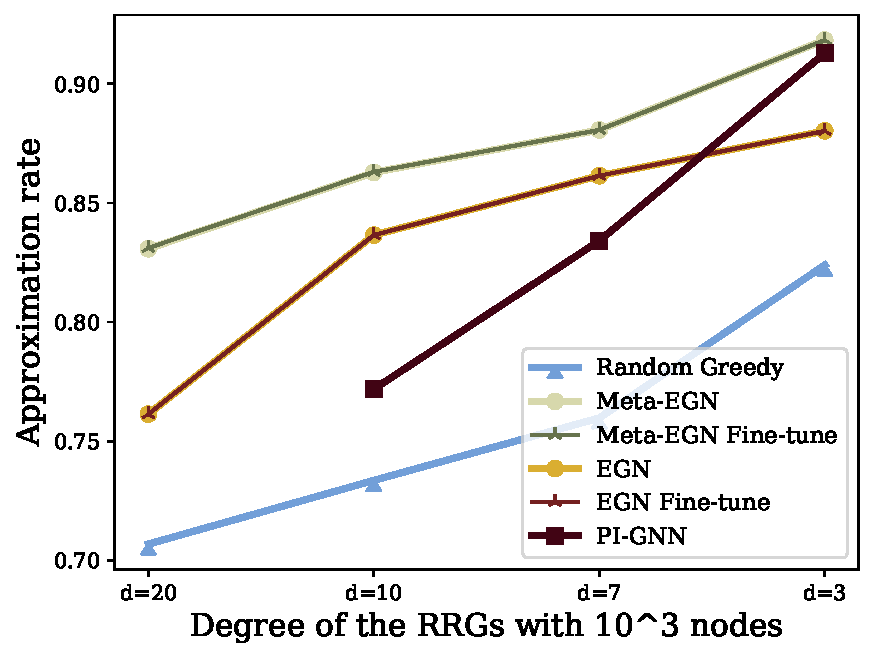
\includegraphics[width=0.32\textwidth]{iclr2023/img/exp/mis_10_3_ga.pdf}
         %\vspace{-0.6cm}
         %\caption{Performance on $10^3$ nodes}
         %\label{fig:mis_ga_103}
     %\end{subfigure}
     \hfill
     %\begin{subfigure}[c]{0.31\textwidth}
         %\centering
         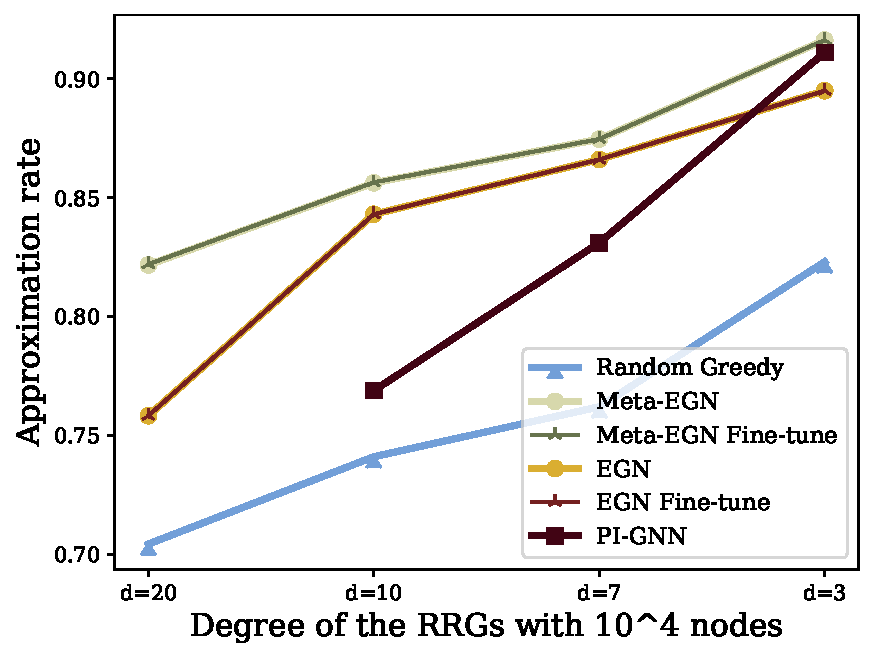
\includegraphics[width=0.32\textwidth]{iclr2023/img/exp/mis_10_4_ga.pdf}
         %\vspace{-0.6cm}
         %\caption{Performance on $10^4$ nodes}
        % \label{fig:mis_ga_104}
     %\end{subfigure}
     \hfill
     %\begin{subfigure}[c]{0.31\textwidth}
         %\centering
         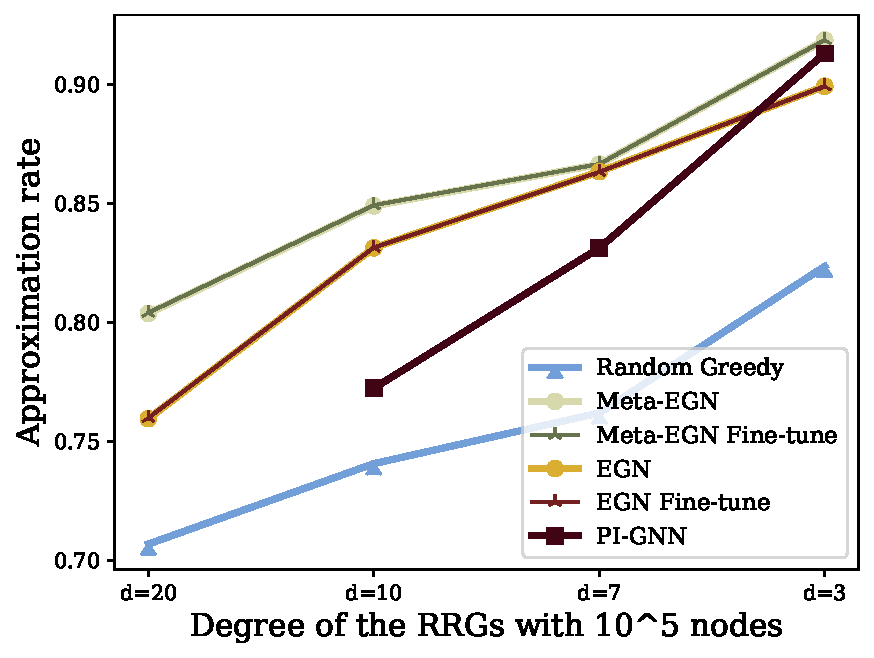
\includegraphics[width=0.32\textwidth]{iclr2023/img/exp/mis_10_5_ga.pdf}
         %\vspace{-0.6cm}
         %\caption{Performance on $10^5$ nodes}
         %\label{fig:mis_ga_105}
     %\end{subfigure}
     \vspace{-0.3cm}
        \caption{ApRs in the MIS problem on RRGs. %\proj and EGN are only trained on RRGs with $1000$ vertices and degrees randomly sampled from $3,7,10,20$. 
        Meta-EGN and EGN are both trained with the output of Random Greedy Algorithm (RGA) as initialization.}
        \label{fig:mis_ga}\vspace{-0.3cm}
\end{figure}


\subsection{\proj boosts the performance with distribution shifts}\label{sec:out-dis}
\textbf{Problem Scale Shift:} Here, we use large-scale RB graphs of 1000-5000 nodes to test EGN and \proj that is trained based on RB500. Table~\ref{tab:mc_generaliztaion_scale} shows the results. Both methods show good generalization while \proj is always better. As the scale increases, Meta-EGN outperforms Gurobi9.5. For example, it takes Meta-EGN with $4$ random initializations only $1.02$s to beat Gurobi9.5 that runs for $3000$ seconds on RB5000 dataset in the MC problem. Moreover, \proj can even outperform Gurobi9.5 on the MVC problem when the problem scale becomes large.

%Meta-EGN improves EGN especially in `Fast' and `Medium' cases with fewer number of random initializations.

%\textbf{Across Scale Generalization:}
%The generalization performance of EGN, Meta-EGN and Gurobi9.5 on extreme hard ($\rho = 0.25$) RB datasets  with vertices ranging from $1000$ to $5000$ of the MC problem are shown in Table~\ref{tab:mc_generaliztaion_scale} and the MVC problem in Table~\ref{tab:mvc_generaliztaion_scale}. The models are only pre-trained on training data with $500$ vertices. Both the unsupervised learning frameworks show good generalization ability with respect to scale changes, Meta-EGN improves EGN especially in `Fast' and `Medium' cases with fewer number of random initializations.
%As the scale increases, Meta-EGN outperforms Gurobi9.5. For example, it takes Meta-EGN with $4$ random initializations only $1.02$s to breakthrough the performance of Gurobi9.5 that has been running for $3000$ seconds on RB5000 dataset in the MC problem.

\textbf{Real-Synthetic Distribution Shift:} Here, we train EGN and \proj on Twitter and test them on RB500.  Table~\ref{tab:generalization_real_synthetic} shows the results. Compare Table~\ref{tab:generalization_real_synthetic} with Tables~\ref{tab:mc_performance},\ref{tab:mvc_performance}. We observe better generalization performance of \proj compared to EGN. For example, for the MC problem, \proj has almost the same performance 
whether there is a dataset shift or not (0.833 v.s. 0.834 before fine-tuning, 0.876 v.s. 0.878  after fine-tuning) while EGN has a bigger gap in performance when there is a shift (0.819 v.s. 0.829 before fine-tuning, 0.831 v.s. 0.864 after fine-tuning). For the MVC problem, although the performance drop of \proj is larger, such a drop is still much smaller than that of EGN.   

%When changing the data distribution, the Meta-EGN models merely pre-trained on source data distribution largely outperform EGN and could even achieve comparable performance with Gurobi9.5, showing its improvement in cross-distribution generalization.

\subsection{Max Independent Set: A response to~\citep{angelini2022cracking}}\label{sec:MIS}


\begin{wrapfigure}{r}{0.38 \linewidth}
\vspace{-7mm}
         \centering
         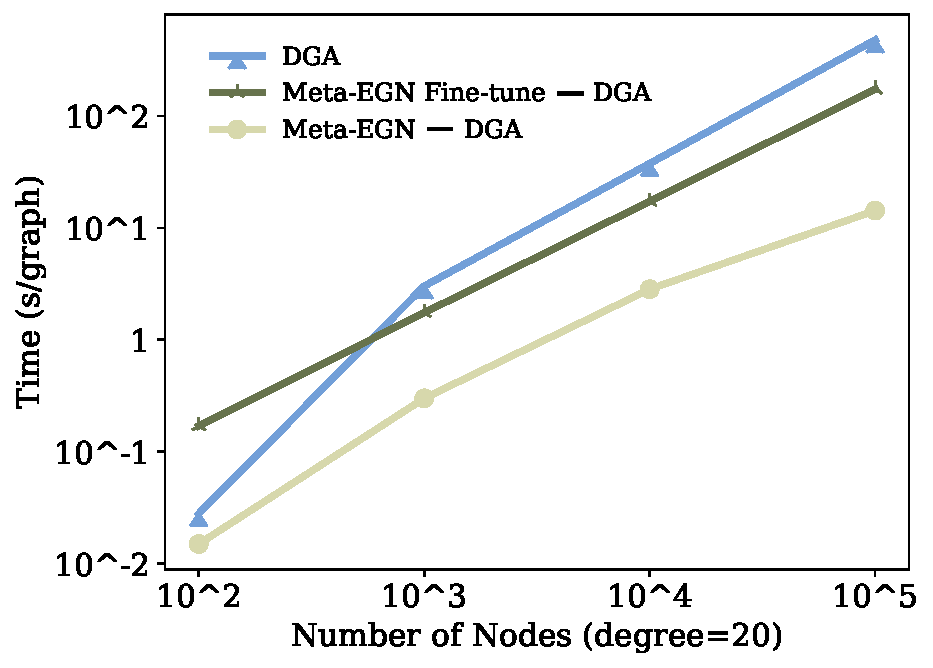
\includegraphics[width=0.38\textwidth]{iclr2023/img/exp/time_20.pdf}
         \vspace{-0.6cm}
         \caption{Time cost v.s. Graph  Scales.}
         \vspace{-0.3cm}
         \label{fig:mis_time}
\end{wrapfigure}


For the MIS problem on large-scale RRGs, ~\cite{angelini2022cracking} have recently posted a concern on learning-based methods by arguing that PI-GNN in~\cite{schuetz2022combinatorial} could not achieve comparable results with the heuristic algorithm DGA~\citep{angelini2019monte}. We see the reason comes from improper usage of learning-based methods in~\cite{schuetz2022combinatorial} as stated in Sec.~\ref{sec:intro}: 1) PI-GNN is trained directly on each single testing instance without learning from the training dataset that contains varies graphs, which is likely to be trapped into the local optima; 2) GNN generally suffers from a node ambiguity issue on RRGs. To resolve the problem, we utilize the outputs of DGA and RGA as the initialization of GNN inputs (EGN, \proj) and expect to learn heuristics from historical data to further tune the solutions given by the greedy algorithms. We train GNN models on RRGs with 1000 nodes with node degrees randomly sampled from $3,7,10,20$, and test on larger RRGs (up to $10^5$ nodes). %To the best of our knowledge, there exists no other non learning-based fine-tuning heuristics that further improves the greedy algorithms for MIS. 
Experiments show that \proj can further improve DGA (in Fig.~\ref{fig:mis}) and RGA (in Fig.~\ref{fig:mis_ga}), while EGN fails to better tune DGA. Note that here EGN and \proj adopt the exactly same backbones. We attribute the improvement to meta-learning-based training as adopted by \proj. See Table~\ref{tab:mis_statistics} in Appendix for more details of the numerical improvement by \proj. We also see in these cases, one-step fine-tuning does not contribute much to the performance of EGN or Meta-EGN, %(i.e. fine-tuning would increase the solution node number by $1$ for every $5$ graphs with degree $20$ and $10^5$ nodes), 
indicating the model before fine-tuning has been very close to a local minimum.

We also check the extra time cost by running \proj to improve DGA solutions in Fig.~\ref{fig:mis_time} and Fig.~\ref{fig:mis_time_app} in Appendix. The extra time cost is just 1\% (without fine-tuning) - 30\% (with fine-tuning) of the time cost of DGA. In theory, the extra time cost without fine-tuning should be $O(|E|)$ for GNN inference plus $O(|V|)$ for rounding, which is in the same order as DGA, while the GNN parallel inference substantially reduces the time.      

%(See Fig.~\ref{fig:mis})(See Fig.~\ref{fig:mis_ga})

%~\cite{angelini2022cracking} have posted a concern that the learning-based method in ~\cite{schuetz2022combinatorial} could not achieve comparable results with the degree-based greedy algorithm (DGA)~\citep{angelini2019monte} in the max independent set (MIS) problem on large scale random regular graphs (RRGs). The reason could be summarized from two aspects: 1) ~\cite{schuetz2022combinatorial} train and test on the same single graphs, which not only requires much time workload given a new testing graph but also makes no use of the heuristics from historical graphs. Thus we pre-train our Meta-EGN on randomly generated datasets with $1000$ vertices for a good initialization, then we either fine-tune the model in one-step or directly infer for time-complexity balance. The time-scale relation is shown in Fig.~\ref{fig:mis_time}, Using GNNs to infer would remain the same time complexity as pure DGA algorithms. 2) The GNNs' limited expressive power~\citep{xu2019powerful} would suffer from severe node ambiguity issue on regular graphs. To resolve the problem, we utilize the output of DGA (See Fig.~\ref{fig:mis}) or GA (See Fig.~\ref{fig:mis_ga}) as the initialization of GNN inputs and expect to learn heuristics to further modify the solution of the greedy algorithms. To the best of our knowledge, there exists no other non learning-based fine-tuning heuristics that further improves the greedy algorithms for MIS. Experiments show that Meta-EGN could improve the performance of both the DGA and GA initialization, while EGN could not outperform DGA even with the DGA initialization. 

%\hl{unfinished}











\iffalse
\subsubsection{max clique:} twitter, collab, IMDB, rbtest, rb500hard, rb1000hard
\subsubsection{vertex covering:} twitter, collab, IMDB, rb500hard, rb1000hard
\pan{I feel that it would be good to have one more setting}
\subsection{Meta brings higher generalization ability}
\subsubsection{from twitter to rb500hard}
max clique + vertex cover
\subsubsection{from rb500 to twitter}
max clique + vertex cover
\subsubsection{Different testing size trained on RB500}
max clique, vertex cover to rb1000hard, rb2000hard
\subsubsection{Different testing difficulty trained on RB500}
max clique, vertex cover
\subsubsection{Real dataset (twitter to other three)}
\subsection{Response to cracking: Meta has the potential to outperform simple baselines}
\hl{unfinished: large scale graphs}
The two charts between nature and cracking

\subsection{Ablation}
\hl{this part is unfinished? (low priority)}
\subsubsection{inner learning rate}
\subsubsection{batch size}



\begin{table}[]
\centering
\fontsize{8}{8}\selectfont
\setlength\tabcolsep{3pt}
\begin{tabular}{@{}ccccccc@{}}
\toprule
\multirow{}{}{} & \multicolumn{2}{c}{COLLAB} & \multicolumn{2}{c}{IMDB} & \multicolumn{2}{c}{RBtest} \\ \cmidrule(l){2-7} 
 & Approximation Rate & Loss Value & Approximation Rate & Loss Value & Approximation Rate & Loss Value \\ \midrule
EGN & 0.980 ± 0.082 & 17.84 & 0.921 ± 0.212 & -12.20 & 0.768 ± 0.061 & 296 \\
Meta-EGN & \textbf{0.995 ± 0.030} & \textbf{-17.81} & \textbf{0.987 ± 0.059} & \textbf{-347.99} & \textbf{0.779 ± 0.065} & \textbf{92.91} \\ \bottomrule
\end{tabular}
\vspace{-0.3cm}
\caption{Twitter to COLLAB, IMDB, RBtest performance on the max clique (MC) problem.}
\vspace{-0.6cm}
\label{tab:generalization_real_real}
\end{table}
\fi



\section{Conclusion}
This work proposes an unsupervised learning framework \proj with the goal of optimizing NNs towards instance-wise good solutions to CO problems. \proj leverages MAML to achieve the goal. \proj views each training instance as a separate task and learns a good initialization for all these tasks. \proj significantly improves the performance of its baseline and has shown good generalization when the data used for training and testing has different scales or distributions.  In addition, \proj can learn to improve the greedy heuristics while paying almost no extra time cost in the problem of maximum independent set on large-scale random regular graphs. 


%To respond to the recent concern on the effectiveness of learning-based methods, \proj can learn to improve greedy heuristics without much extra time cost complexity in the MIS on large scale RRGs. 

%By taking a graph instance as the input, \porh

%By learning its meta-learning objective, \proj learns from historical graphs for better initialization as well as do fine-tuning to further approach the optimality of each instance. The one-step fine-tuning enables \proj an even wider performance guarantee compared with the previous methods. \proj significantly improves the performance of its baseline even before the fine-tuning step and also has better generalization across scale or data distribution changes. In addition, \proj improves the greedy heuristics as well as maintain the time complexity in the MIS on large scale RRGs. 



%In the future, we aim to further modify \proj in the problems that require global assignment  and broaden \proj to fine-tune more heuristics or approximation methods.


%fill in the gap between the actual goal of CO problems (to achieve optimality for every single instance) and the optimization objective adopted by previous unsupervised learning for CO (the optimality in the averaged sense), and proposes \proj, a meta-learning based unsupervised learning for CO framework. \proj aims to learn better heuristics from the historical graphs for better initialization and do further fine-tuning on the testing instances to move closer towards the optimality for the single instance. The one-step fine-tuning enables \proj an even wider performance guarantee compared with the previous methods.
%\proj significantly improves the performance of its baselines in the max clique problem and the minimum vertex covering problems on both real and synthetic datasets, even before the fine-tuning step. Experiments show that \proj has better generalization across scale and data distribution. In addition, the work utilizes \proj to learn to further improve the performance of heuristics as well as maintain the time complexity in the max independent set problem on large scale random-regular graphs, as a response to ~\cite{angelini2022cracking}. In the future, we aim to further improve \proj in global assignment problems and broaden \proj to fine-tune more heuristics or approximation methods.

\iffalse
\subsection{Limitations}
\proj on all the MC baselines and boost their performance? Because SA or PT requires carefully tuned. leave it for further study.
\fi

\section{Acknowledgement}
We would like to express our deepest appreciation to Dr. Tianyi Chen for the insightful discussion on the meta-learning framework from a theoretical aspect and Dr. Ruqi Zhang for the constructive advice on the fine-tuning strategies. We would also like to extend our deepest gratitude to Dr. Hanjun Dai and Dr. Jialin Liu for sharing their invaluable insights into the general ideas of learning for combinatorial optimization. Also many thanks to our funding, H. Wang and P. Li are partially supported by 2021
JPMorgan Faculty Award and the NSF award OAC-2117997. 



%\newpage

\bibliography{iclr2023_conference}
\bibliographystyle{iclr2023_conference}

\appendix
%\newpage
%\section{Appendix}
\section{Proof of Theorem~\ref{thm:general_alpha}}
\label{sec:proof-performance_guarantee}

We first prove Theorem~\ref{thm:general_alpha}, then we specify the value of $\alpha$ to obtain Theorem~\ref{thm:thm_performance_guarantee} as a specific case of Theorem~\ref{thm:general_alpha}. The proof of Theorem~\ref{thm:general_alpha} is divided into two parts. 

In part 1, we prove that if \underline{$l(\theta;G) < \beta + \triangle$ (even if $l(\theta;G) \geq \beta$)}, for any $\alpha \in (0, 2/L)$ Meta-GNN with one-step finetuning outputs \underline{a feasible solution $X$ of good quality} $f(X;G)\leq l(\theta;G)-\triangle$. Here, $\triangle = \|\nabla_{\theta} l(\theta;G)\| \epsilon + \frac{1}{2L\alpha^2 - 4\alpha}\epsilon^2$ if $\epsilon < \alpha \|\nabla_{\theta} l(\theta;G)\|$ or $\triangle = (\alpha - \frac{L\alpha^2}{2})\|\nabla_{\theta}l(\theta;G)\|^2$ o.w..

In part 2, we prove that once \proj achieves the loss value $l(\theta';G)$ after the one-step finetuning, the rounding process would output a feasible $X$ whose objective satisfies $f(X;G)\leq l(\theta';G)$. 

\textbf{Part 1:}We could get 
\begin{equation}
\begin{aligned}
l(\theta';G) 
& \stackrel{(a)}{\leq} l(\theta;G) + \nabla_{\theta}l(\theta;G)(\theta'-\theta) + \frac{1}{2}L \| \theta' - \theta\|_2^2\\
& \stackrel{(b)}{=} l(\theta;G) + \frac{1}{2}L\|\theta' - \theta\|_2^2 - \alpha \|\nabla_{\theta} l(\theta;G)\|_2^2 \\
&  = l(\theta;G)+ (\frac{L\alpha^2}{2} - \alpha) \|\nabla_{\theta} l(\theta;G)\|_2^2,
\end{aligned}
\end{equation}
where (a) is due to the local L-smoothness of $l(\cdot;G)$, (b) is due to the definition of one-step finetuning $\theta' = \theta - \alpha \nabla_{\theta}l(\theta;G)$.

If $\epsilon < \alpha \|\nabla_{\theta}l(\theta;G)\|$:

\qquad Let $\triangle = \|\nabla_{\theta} l(\theta;G)\| \epsilon + \frac{1}{2L\alpha^2 - 4\alpha}\epsilon^2$, we have:
\begin{equation}
\begin{aligned}
\min_{\epsilon} - \triangle & = \min_{\epsilon} -\frac{1}{2L\alpha^2 - 4\alpha} \epsilon^2 - \|\nabla_{\theta}l(\theta;G)\|\epsilon  = (\frac{L\alpha^2}{2}-\alpha)\|\nabla_{\theta}l(\theta;G)\|^2,
\end{aligned}
\end{equation}

\qquad thus
\begin{equation}
\begin{aligned}
    l(\theta';G) &\leq l(\theta;G) - \triangle.
\end{aligned}
\end{equation}

If $\epsilon \geq \alpha \|\nabla_{\theta}l(\theta;G)\|$:

\qquad Let $\triangle = (\alpha - \frac{L\alpha^2}{2})\|\nabla_{\theta}l(\theta;G)\|^2$, we would directly have:
\begin{equation}
\begin{aligned}
    l(\theta';G) &\leq l(\theta;G) - \triangle.
\end{aligned}
\end{equation}
By this, we finish the first part of the proof for Theorem~\ref{thm:general_alpha}. 

\textbf{Part 2:} The proof in this part follows the rounding analysis in ~\cite{wang2022unsupervised}. Consider the rounding procedure from continuous space $\bar{X} = \mathcal{A}_{\theta}(G), \bar{X} \in [0,1]^n$ into the discrete feasible solution $X \in \{0,1\}^n$. Let $\bar{X}_i, X_i, i = \{0,1,...,n\}$ denote their entries. W.l.o.g, suppose the rounding order is from $1$ to $n$ and we have finished the rounding before the $t$-th node, we now analyze the rounding of $t$-th node:
\begin{equation}
\begin{aligned}
    %& l(\theta';G) \\
    & f_r([X_1,...,X_{t-1},\bar{X}_t,\bar{X}_{t+1},...,\bar{X}_n];G) + \beta g_r([X_1,...,X_{t-1},\bar{X}_t,\bar{X}_{t+1},...,\bar{X}_n];G) \\
      \stackrel{(d)}{\geq} & \bar{X}_t ( f_r([X_1,...,X_{t-1},1,\bar{X}_{t+1},...\bar{X}_n];G) + \beta g_r([X_1,...,X_{t-1},1,\bar{X}_{t+1},...,\bar{X}_n];G)) \\
    & + (1-\bar{X}_t) ( f_r([X_1,...,X_{t-1},0,\bar{X}_{t+1},...,\bar{X}_n];G) + \beta g_r([X_1,...,X_{t-1},0,\bar{X}_{t+1},...,\bar{X}_n];G)) \\
    \geq & \bar{X}_t ( \min_{j_t=\{0,1\}}f_r([X_1,...,X_{t-1},j_t,\bar{X}_{t+1},...,\bar{X}_n];G) + \beta g_r([X_1,...,X_{t-1},j_t,\bar{X}_{t+1},...,\bar{X}_n];G)) \\
    & + (1-\bar{X}_t) (\min_{j_t=\{0,1\}} f_r([X_1,...,X_{t-1},j_t,\bar{X}_{t+1},...,\bar{X}_n];G) \\
    &+ \beta g_r([X_1,...,X_{t-1},j_t,\bar{X}_{t+1},...,\bar{X}_n];G)) \\
     \stackrel{(e)}{=} & f_r([X_1,...,X_{t-1},X_t,\bar{X}_t,...,\bar{X}_n];G) + \beta g_r([X_1,...,X_{t-1},X_t,\bar{X}_t,...,\bar{X}_n];G) \\
\end{aligned}
\end{equation}
where (d) is due to $l_r(\theta;G)$'s entry-wise concavity w.r.t $\bar{X}$ and Jensen's inequality, (e) is due to $X_t = \arg\min_{j=0,1} f_r(X_1,...,X_{t-1},t,\bar{X}_{t+1},...,\bar{X}_n)+\beta g_r(X_1,...,X_{t-1},t,\bar{X}_{t+1},...,\bar{X}_n)$ (the definition of our rounding process). The loss value is monotonically non-increasing through the whole rounding process according to the equation above, thus we could get:
\begin{equation}
    l(\theta') \geq f(X;G) + \beta g(X;G)
\end{equation}
By this, we finish the proof of the second part.

\subsection{A Specific Case}
Note that in the first part of the proof above, if we specify the value of $\alpha$ as $\frac{1}{L}$ in equation (6), we could have:
\begin{equation}
    l(\theta';G) \leq l(\theta;G) -\frac{\|\nabla_{\theta}l(\theta;G)\|_2^2}{2L} 
\end{equation}
If $\epsilon< \frac{1}{L}\|\nabla_{\theta} l(\theta;G)\|$:

\qquad Let $\triangle = \|\nabla_{\theta}l(\theta;G)\| \epsilon - \frac{L}{2}\epsilon^2$, we have: 

\begin{equation}
\begin{aligned}
\min_{\epsilon} - \triangle & = \min_{\epsilon} \frac{L}{2} \epsilon^2 - \|\nabla_{\theta}l(\theta;G)\|\epsilon  = -\frac{\|\nabla_{\theta}l(\theta;G)\|^2}{2L},
\end{aligned}
\end{equation}
\qquad thus
\begin{equation}
\begin{aligned}
    l(\theta';G) &\leq l(\theta;G) - \triangle.
\end{aligned}
\end{equation}


If $\epsilon \geq \frac{1}{L}\|\nabla_{\theta} l(\theta;G)\|$:

\qquad Let $\triangle = \frac{1}{2L}\|\nabla_{\theta}l(\theta;G)\|^2$, we would directly have:
\begin{equation}
\begin{aligned}
    l(\theta';G) &\leq l(\theta;G) - \triangle.
\end{aligned}
\end{equation}
By this, we obtain Theorem~\ref{thm:thm_performance_guarantee}, a specific case of Theorem~\ref{thm:general_alpha} as follows:

\begin{theorem}[A Specific case of Theorem~\ref{thm:general_alpha}]
\label{thm:thm_performance_guarantee}
Suppose the relaxations $f_r$ and $g_r$ are entry-wise concave as required in \citep{wang2022unsupervised}. Let $\theta$ denote the learned parameter after training.  Given a test instance $G$, suppose locally $l(\cdot;G)$ is $L$-smooth at $\theta$, i.e., $\|\nabla_{\theta'} l(\theta';G) - \nabla_{\theta} l(\theta;G)\|\leq L\|\theta' - \theta\|$ for all $\theta'$ that satisfies $\|\theta' - \theta\|\leq \epsilon$. Then, if \underline{$l(\theta;G) < \beta + \triangle$ (even if $l(\theta;G) \geq \beta$)}, there exists $\alpha$ such that Meta-GNN with one-step finetuning outputs \underline{a feasible solution $X$ of good quality} $f(X;G)\leq l(\theta;G)-\triangle$. Here, $\triangle = \|\nabla_{\theta} l(\theta;G)\|\epsilon - \frac{L}{2}\epsilon^2$ if $\epsilon< \frac{1}{L}\|\nabla_{\theta} l(\theta;G)\|$ or $\triangle=\frac{1}{2L}\|\nabla_{\theta} l(\theta;G)\|^2$ o.w..
\end{theorem}


\vspace{0.2cm}


\iffalse
\subsection{Theorem ~\ref{thm:thm_performance_guarantee}: A More General Case}
In Theorem~\ref{thm:thm_performance_guarantee}, we proved the performance guarantee of \proj when the inner learning rate $\alpha$ is set as $1/L$ as the best case. Here we extend the value of $\alpha$ into general cases and show that our theorem still holds.

\begin{theorem}[General case for Theorem~\ref{thm:thm_performance_guarantee}]
\label{thm:general_alpha2}
Suppose the relaxations $f_r$ and $g_r$ are entry-wise concave as required in \citep{wang2022unsupervised}. Let $\theta$ denote the learned parameter after training.  Given a test instance $G$, suppose locally $l(\cdot;G)$ is $L$-smooth at $\theta$, i.e., $\|\nabla_{\theta'} l(\theta';G) - \nabla_{\theta} l(\theta;G)\|\leq L\|\theta' - \theta\|$ for all $\theta'$ that satisfies $\|\theta' - \theta\|\leq \epsilon$. Then, if \underline{$l(\theta;G) < \beta + \triangle$ (even if $l(\theta;G) \geq \beta$)}, for any $\alpha \in (0, 2/L)$ Meta-GNN with one-step finetuning outputs \underline{a feasible solution $X$ of good quality} $f(X;G)\leq l(\theta;G)-\triangle$. Here, $\triangle = \|\nabla_{\theta} l(\theta;G)\| \epsilon + \frac{1}{2L\alpha^2 - 4\alpha}\epsilon^2$ if $\epsilon < \alpha \|\nabla_{\theta} l(\theta;G)\|$ or $\triangle = (\alpha - \frac{L\alpha^2}{2})\|\nabla_{\theta}l(\theta;G)\|^2$ o.w..
\end{theorem}

\textbf{Proof of Theorem~\ref{thm:general_alpha}:} We divide our proof into two parts. In part 1, we prove that . In part 2, we need to prove that once \proj achieves the loss value $l'(\theta;G)$ after the one-step finetuning, the rounding process would output a feasible solution such that $f(X;G)\leq l(\theta';G)$. The proof of part 2 is exactly the same as that for Theorem~\ref{thm:thm_performance_guarantee}, therefore we only provided the details of part 1 as follows:
By Taylor Expansion, we could get 
\begin{equation}
\begin{aligned}
l(\theta';G) 
& \stackrel{(a)}{\leq} l(\theta;G) + \nabla_{\theta}l(\theta;G)(\theta'-\theta) + \frac{1}{2}L \| \theta' - \theta\|_2^2\\
& \stackrel{(b)}{=} l(\theta;G) + \frac{1}{2}L\|\theta' - \theta\|_2^2 - \alpha \|\nabla_{\theta} l(\theta;G)\|_2^2 \\
&  = l(\theta;G)+ (\frac{L\alpha^2}{2} - \alpha) \|\nabla_{\theta} l(\theta;G)\|_2^2,
\end{aligned}
\end{equation}
where (a) is due to the local L-smoothness of $l(\cdot;G)$, (b) is due to the definition of one-step finetuning $\theta' = \theta - \alpha \nabla_{\theta}l(\theta;G)$.

If $\epsilon < \alpha \|\nabla_{\theta}l(\theta;G)\|$:

\qquad Let $\triangle = \|\nabla_{\theta} l(\theta;G)\| \epsilon + \frac{1}{2L\alpha^2 - 4\alpha}\epsilon^2$, we have:
\begin{equation}
\begin{aligned}
\min_{\epsilon} - \triangle & = \min_{\epsilon} -\frac{1}{2L\alpha^2 - 4\alpha} \epsilon^2 - \|\nabla_{\theta}l(\theta;G)\|\epsilon  = (\frac{L\alpha^2}{2}-\alpha)\|\nabla_{\theta}l(\theta;G)\|^2,
\end{aligned}
\end{equation}

\qquad thus
\begin{equation}
\begin{aligned}
    l(\theta';G) &\leq l(\theta;G) - \triangle.
\end{aligned}
\end{equation}

If $\epsilon \geq \alpha \|\nabla_{\theta}l(\theta;G)\|$:

\qquad Let $\triangle = (\alpha - \frac{L\alpha^2}{2})\|\nabla_{\theta}l(\theta;G)\|^2$, we would directly have:
\begin{equation}
\begin{aligned}
    l(\theta';G) &\leq l(\theta;G) - \triangle.
\end{aligned}
\end{equation}
\fi

\section{Supplementary Experiment Results}
\subsection{Supplementary Time cost v.s. Graph Scale in the MIS}
we show the degree $3,7,10$ in the following Fig.~\ref{fig:mis_time_app}. They show the same time-cost vs scale relation as that in Fig.~\ref{fig:mis_time}. The extra time cost of GNN is $O(|E|)$ for inference plus $O(|V|)$ for rounding, which is in the same order of DGA.

\begin{figure}[h]
     \centering
     %\begin{subfigure}[c]{0.31\textwidth}
         %\centering
         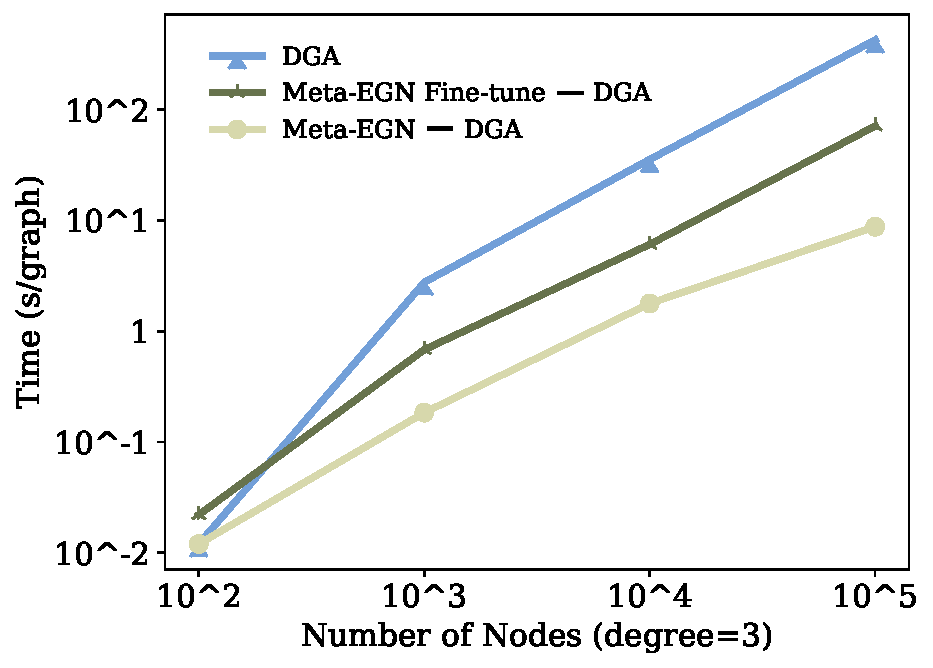
\includegraphics[width=0.32\textwidth]{iclr2023/img/exp/time_3.pdf}
         %\vspace{-0.6cm}
         %\caption{Performance on $10^3$ nodes}
         %\label{fig:mis_ga_103}
     %\end{subfigure}
     \hfill
     %\begin{subfigure}[c]{0.31\textwidth}
         %\centering
         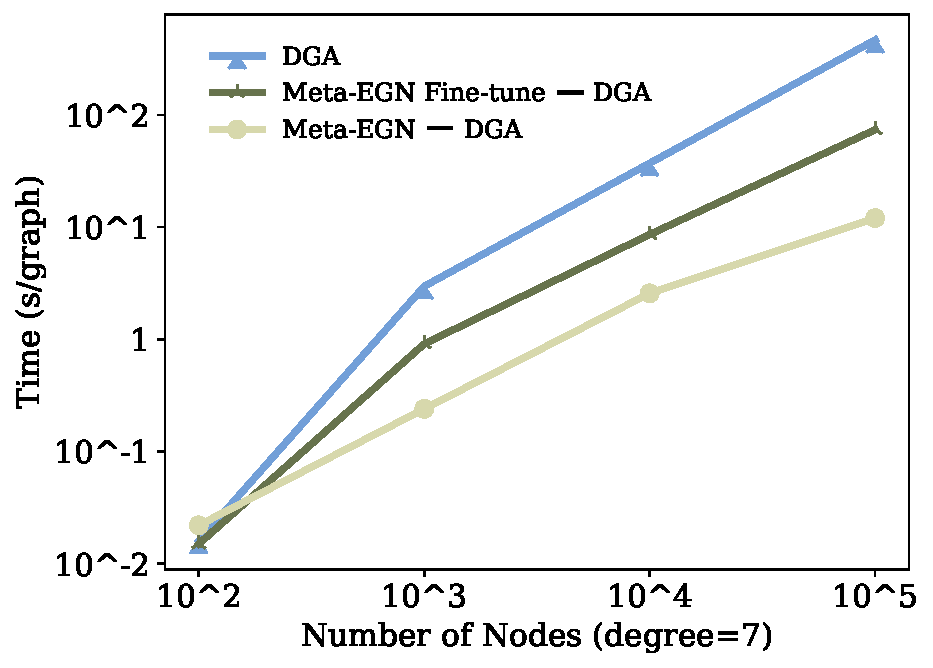
\includegraphics[width=0.32\textwidth]{iclr2023/img/exp/time_7.pdf}
         %\vspace{-0.6cm}
         %\caption{Performance on $10^4$ nodes}
        % \label{fig:mis_ga_104}
     %\end{subfigure}
     \hfill
     %\begin{subfigure}[c]{0.31\textwidth}
         %\centering
         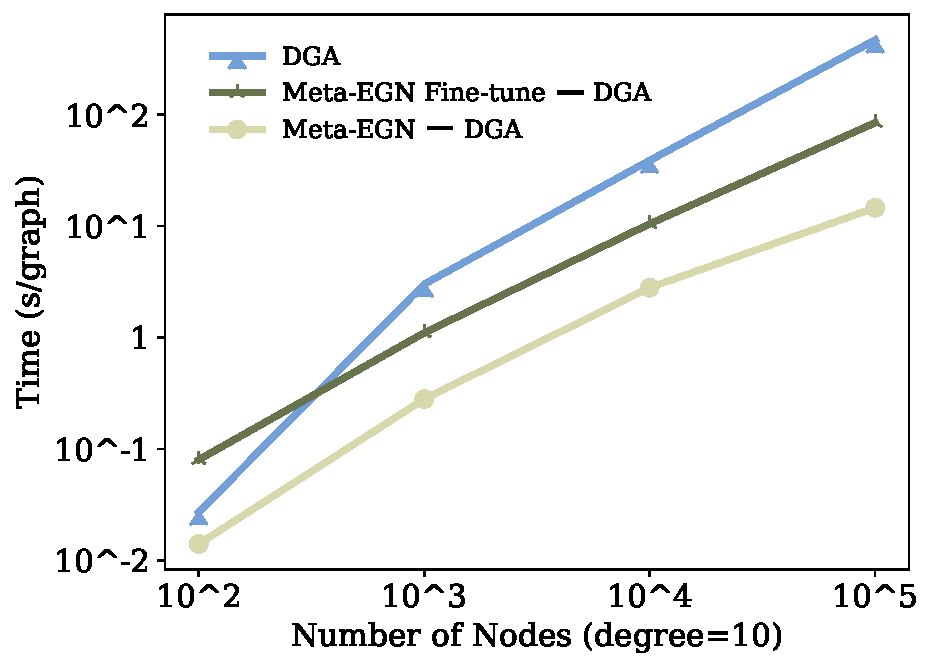
\includegraphics[width=0.32\textwidth]{iclr2023/img/exp/time_10.pdf}
         %\vspace{-0.6cm}
         %\caption{Performance on $10^5$ nodes}
         %\label{fig:mis_ga_105}
     %\end{subfigure}
     \vspace{-0.3cm}
        \caption{Time cost v.s. Graph Scales on degree $3,7,10$}
        \label{fig:mis_time_app}
\end{figure}
\subsection{How much does \proj modify DGA and RGA heuristics in the MIS}
%We provide the details that how much \proj could further modify the two heuristics DGA and RGA, as shown in Table.~\ref{tab:mis_statistics}.
We display the average approximation rate improvement and the average node number increase by Meta-EGN over DGA and RGA in Table.~\ref{tab:mis_statistics}.
\begin{table}[h]
\caption{Improvement of \proj over DGA and RGA in the MIS on RRGs, `Imp in ApR' denotes the average improvement in approximation rate, and `Imp in $\#$Node' denotes the average number of nodes that \proj could find more than the heuristics.}
\label{tab:mis_statistics}
\vspace{-0.3cm}
\resizebox{1.0\textwidth}{!}{\begin{tabular}{@{}cccc|cc|cc|cc@{}}
\toprule
 & \multirow{2}{*}{Scale$/$Degree} & \multicolumn{2}{c|}{3} & \multicolumn{2}{c|}{7} & \multicolumn{2}{c|}{10} & \multicolumn{2}{c}{20} \\ \cmidrule(l){3-10} 
 &  & Imp in ApR & Imp in $\#$Node & Imp in ApR & Imp in $\#$Node & Imp in ApR & Imp in $\#$Node & Imp in ApR & Imp in $\#$Node \\ \midrule
\multirow{3}{*}{\proj improves DGA by} & $10^3$ & 0.0043 & 1.950 & 0.0060 & 2.014 & 0.0044 & 1.254 & 0.0084 & 1.657 \\
 & $10^4$ & 0.0050 & 22.768 & 0.0062 & 20.811 & 0.0067 & 19.109 & 0.0079 & 15.588 \\
 & $10^5$ & 0.0032 & 145.718 & 0.0045 & 151.051 & 0.0051 & 145.69 & 0.0050 & 98.660 \\ \midrule
\multirow{3}{*}{\proj improves RGA by} & $10^3$ & 0.0944 & 42.986 & 0.1208 & 40.549 & 0.1292 & 36.849 & 0.1239 & 24.447 \\
 & $10^4$ & 0.0932 & 424.404 & 0.1125 & 377.628 & 0.1151 & 328.276 & 0.1173 & 231.456 \\
 & $10^5$ & 0.0871 & 3966.272 & 0.1045 & 3507.751 & 0.1083 & 3088.824 & 0.0969 & 1912.030 \\ \bottomrule 
\end{tabular}}
\end{table}

\subsection{Training the Models on Subsets of the Training Data}
We display the average approximation rates of the models that are only trained on subsets of the original training data in the max clique problem on Twitter. The training dataset is randomly sampled from the original training dataset and the testing dataset remains the same as that in Table.~\ref{tab:mc_performance}. Both methods have worse performance as the number of training instances reduces, while Meta-EGN only has a $0.7\%$ performance decrease from the full-size training dataset with 750 samples to the training subset with only $64$ instances. In contrast, EGN decreases its performance by $1.7\%$.


\begin{table}[h]
\caption{The approximation rate of the max clique problem on Twitter. Models are only trained on subsets of the dataset, `training subset' denotes the number of instances in the training data.}
\centering
\begin{tabular}{@{}cccccc@{}}
\toprule
training subset & 64          & 128         & 256         & 512         & Full (750)  \\ \midrule
EGN           & 0.909±0.122 & 0.911±0.118 & 0.914±0.118 & 0.922±0.115 & 0.926±0.113 \\
Meta-EGN      & 0.970±0.058 & 0.973±0.055 & 0.975±0.055 & 0.975±0.051 & 0.976±0.048 \\ \bottomrule
\end{tabular}
\end{table}

\subsection{Training the Models on RRGs with single Degrees in the MIS}
We train the EGN and Meta-EGN models on RRGs with only $3$ or $20$ degrees and test them on RRGs with the rest of degrees from $\{3, 7, 10, 20\}$. Models take the output of DGA as the initialization graph node feature. We show the performance of both the models without fine-tuning in Fig.~\ref{fig:train_only3_20}. When only trained on RRGs with degree $3$ (See the left two figures in Fig.~\ref{fig:train_only3_20}), both the models could not generalize well, as neither of them could outperform the initialization input of DGA. Note that Meta-EGN still achieves better performance than EGN in this case. As to the models only trained on RRGs with degree $20$ (See the right two figures in Fig.~\ref{fig:train_only3_20}), we observe that both the model have relatively good generalization ability across different degrees, yet Meta-EGN could still marginally outperform EGN in this case. We attribute this phenomenon to the fact that solving the MIS on RRGs with degree $20$ is much more complicated than those with degree $3$ and thus may contain adequate heuristics for solving RRGs with lower degrees.


\begin{figure}[h]
     \centering
         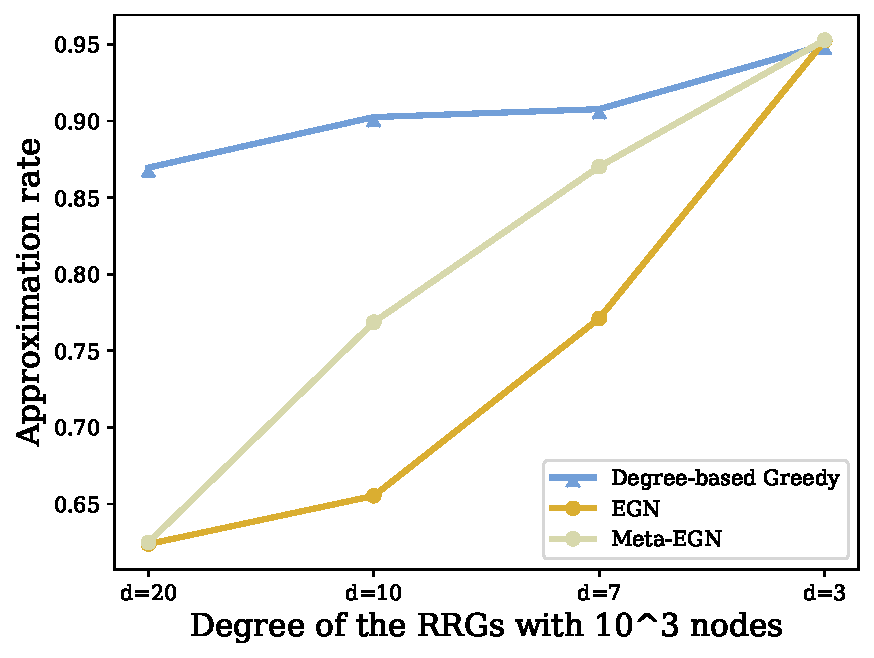
\includegraphics[width=0.23\textwidth]{iclr2023/img/app/mis_10_3_app3.pdf}
     \hfill
         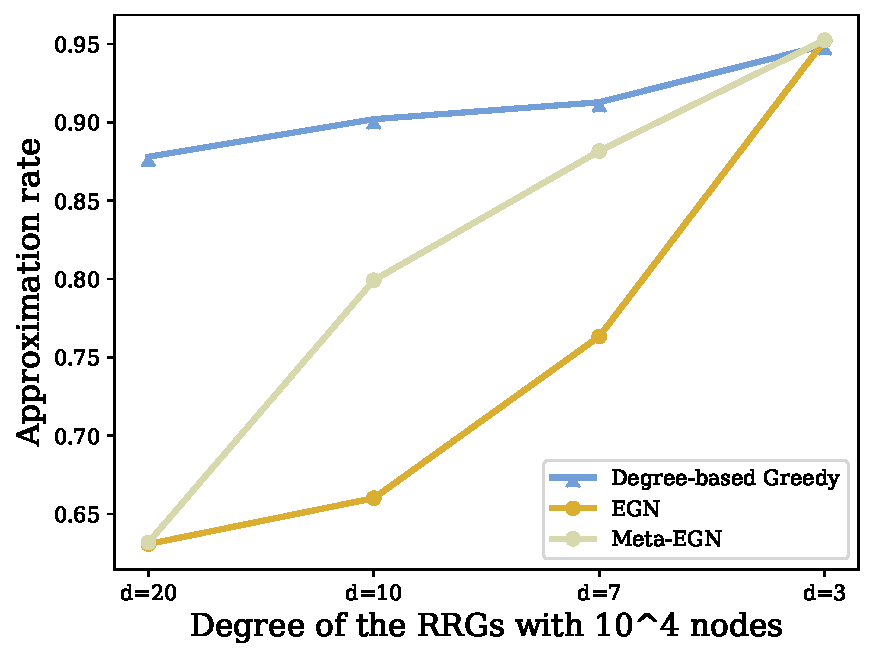
\includegraphics[width=0.23\textwidth]{iclr2023/img/app/mis_10_4_app3_.pdf}
     \hfill
         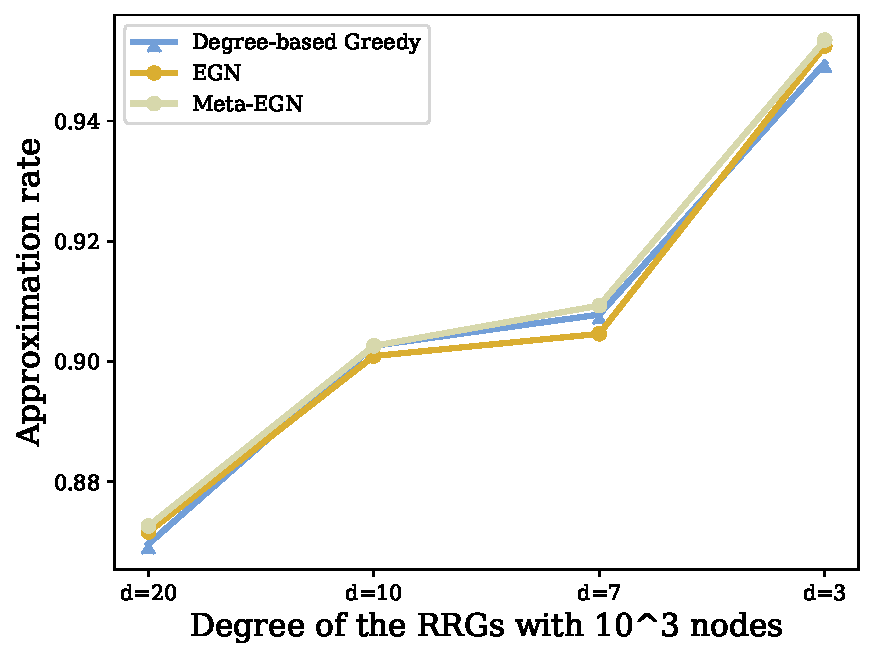
\includegraphics[width=0.23\textwidth]{iclr2023/img/app/mis_10_3_app20.pdf}
    \hfill
        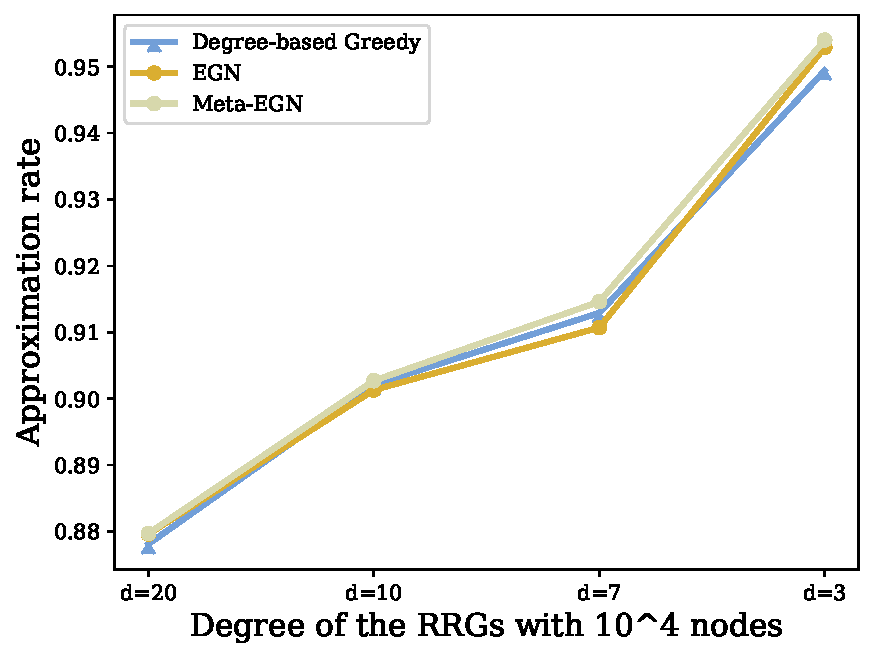
\includegraphics[width=0.23\textwidth]{iclr2023/img/app/mis_10_4_app20.pdf}
     \vspace{-0.3cm}
        \caption{The left two figures show the ApRs on RRGs with $10^3$ and $10^4$ nodes of the models trained only on RRGs with degree $3$. The right two figures show the ApRs on RRGs with $10^3$ and $10^4$ nodes of the models trained only on RRGs with degree $20$.}
        \label{fig:train_only3_20}
        \vspace{-0.3cm}
\end{figure}

\subsection{Comparison on the Training Time of the Models}
We display the wall clock training time for the two methods to converge in Table.~\ref{tab:training_time} (from start to the best epoch on validation set). We observe that Meta-EGN generally takes two to three times to converge compared with EGN, but their training time cost basically remains on the same order of magnitude.

\begin{table}[h]
\caption{The wall clock training time to convergence of EGN and Meta-EGN in different problems.}
\label{tab:training_time}
\centering
\begin{tabular}{@{}cccc|ccc|c@{}}
\toprule
\multirow{2}{*}{\begin{tabular}[c]{@{}c@{}}Dataset/Time\\ (min:second)\end{tabular}} & \multicolumn{3}{c|}{MC} & \multicolumn{3}{c|}{MVC} & MIS \\
 & Twitter & RB200 & RB500 & Twitter & RB200 & RB500 & RRGs \\ \midrule
EGN & 46:50 & 104:37 & 282:57 & 100:58 & 83:27 & 128:39 & 733:02 \\
Meta-EGN & 101:55 & 210:04 & 609:47 & 276:38 & 168:25 & 282:15 & 1088:55 \\ \bottomrule
\end{tabular}
\end{table}
\section{Supplementary Implementation Details}
\label{sec:app_experiment_details}
\subsection{Experiment Details}
All the codes run on the PyTorch platform 1.9.0~\citep{NEURIPS2019_9015} and PyTorch Geometric framework 1.7.2~\citep{Fey/Lenssen/2019}. The details of each dataset is shown in Table.~\ref{tab:dataset_details}, all of the real datasets are publicly available, and we follow the code in~\citep{toenshoff2021graph} to generate the RB model.
\begin{table}[h]
\caption{The number of instances in each dataset. `20/scale/degree' means that we generate $20$ testing instances for each different scale-degree pair. We generate RB1000, RB2000, and RB5000 only for testing.}
\vspace{-0.2cm}
\label{tab:dataset_details}
\resizebox{1.0\textwidth}{!}{\begin{tabular}{@{}cccccccccc@{}}
\toprule
Dataset & Twitter & COLLAB & IMDB & RB200 & RB500 & RB1000 & RB2000 & RB5000 & RRGs \\ \midrule
Training & 750 & 3600 & 800 & 2000 & 2000 & - & - & - & 3000 \\
Validation & 100 & 450 & 100 & 100 & 100 & - & - & - & 30 \\
Testing & 100 & 450 & 100 & 100 & 100 & 100 & 100 & 100 & 20/scale degree \\ \bottomrule
\end{tabular}}
\end{table}

To balance the training time per epoch of EGN and Meta-EGN, we define the epoch as follows: For each epoch of EGN training, the whole dataset is split into mini-batches. EGN performs standard mini-batch training along these batches and optimizes over each mini-batch. As to Meta-EGN, for each training epoch Meta-EGN only randomly samples a single batch and does the meta learning algorithm on the batch. The batch sizes of the methods are controlled the same.

\subsection{Detailed Derivation of the Loss Function Relaxation}
In this part, we display the detailed loss function relaxation of the three problems in our study (the MC, the MVC, and the MIS). The basic idea of training loss design and relaxation follow ~\citep{karalias2020erdos,wang2022unsupervised}.
In the following derivation, we use $i,j$ to represent the nodes in graphs, we use $X_i, X_j \in \{0,1\}$ to denote the discrete assignment of the binary optimization variables, and we use $\bar{X}_i, \bar{X}_j \in [0,1]$ to denote the relaxed soft assignment of the binary optimization variables.

\textbf{The maximum clique (MC):} A clique is a set of nodes $S\in V$ such that any two distinct nodes in the set are adjacent. The MC aims to find out the clique with the largest number of nodes. We could formulated the optimization objective as follows:
\begin{equation}
\centering
    \max_{X}  \sum_{1\leq i\leq n} X_i  \quad \quad \text{s.t.} \quad  (i, j) \in E\;\text{if}\;{X_i, X_j = 1} ,
\end{equation}$X_i,X_j$ denotes whether to take the node into the clique set ($X_i = 1$) or not ($X_i = 0$). By setting a proper penalty coefficient $\beta$, we could formulate the loss function relaxation as follows (the detailed derivation follows the corresponding case study in ~\cite{karalias2020erdos}).
\begin{equation}
    l_{\text{MC}}(\theta;G) \triangleq - (\beta+1)\sum_{(i,j)\in E} \bar{X}_i \bar{X}_j + \frac{\beta}{2} \sum_{i \neq j} \bar{X}_i \bar{X}_j.
\end{equation}

\textbf{The minimum vertex covering (MVC):} A vertex cover is a set of nodes $S\in V$ that any edge in the graph is connected to at least a node from the set. The MVC aims to find out the cover set with the smallest number of nodes. The optimization objective could be summarized as follows:
\begin{equation}
    \min_{X} \sum_{1 \leq i \leq n} X_i \quad \quad \text{s.t.} \quad  X_i + X_j \geq 1\;\;\text{if}\;(i,j)\in E,
\end{equation}where $X_i,X_i$ denotes whether to take the node into the cover set ($X_i = 1$) or not ($X_i=0$). We design the constraint function $g$ to represent the total number of edges that have not been covered given a set of variable assignment $X$, and thus we write $g$ as:
\begin{equation}
    g_{\text{MVC}}(X;G) \triangleq \sum_{(i,j) \in E} (1-X_i) (1-X_j).
\end{equation}
Then we relax the constraint $g$ and add it into the training objective by multiplying a proper penalty coefficient $\beta$, following the relaxation principle in~\cite{wang2022unsupervised}:
\begin{equation}
    l_{\text{MVC}}(\theta;G) \triangleq \sum_{1\leq i \leq n} \bar{X}_i +\beta \sum_{(i,j) \in E} (1-\bar{X}_i) (1-\bar{X}_j).
\end{equation}
By this, we aim to minimize the value of the loss function above in order to minimize the node number of the cover set as well as consider the covering property in the constraint.


\textbf{The maximum independent set (MIS):} An independent set is a set of nodes where any two distinct nodes in the set are not adjacent to each other. The MIS aims to find out the independent set with the largest number of nodes. We could formulate the objective of the MIS as follows:
\begin{equation}
    \max_{X} \sum_{1 \leq i \leq n} X_i \quad \quad \text{s.t.} \quad  X_iX_j = 0 \;\text{if}\; (i,j) \in E,
\end{equation}where $X_i, X_j$ denotes whether to take the node into the independent set ($X_i = 1$) or not ($X_i = 0$). We formulate the constraint $g$ as the total number of edges whose two connected nodes at the end points are both assigned into the independent set. Therefore we could write the constraint as follows:
\begin{equation}
    g_{\text{MIS}} \triangleq \sum_{(i,j) \in E} X_i X_j.
\end{equation}
We then relax the constraint $g$ into continuous space and add it into the c function with a proper penalty coefficient $\beta$, following the relaxation principle in ~\citep{wang2022unsupervised}, and thus we could write the training loss function as:
\begin{equation}
    l_{\text{MIS}}(\theta;G) \triangleq -\sum_{1 \leq i \leq n} \bar{X}_i + \beta \sum_{(i,j) \in E} \bar{X_i} \bar{X_j}.
\end{equation}
By this, we aim to minimize the value of the loss function above in order to maximize the node number of the independent set as well as consider the independent property in the constraint.

\subsection{Separated Algorithm Tables}
We separate the algorithm table of \proj into training and testing parts to make it clearer. The algorithm table is shown in Alg.~\ref{method:alg_table_train} for training and Alg.~\ref{method:alg_table_test}.

\begin{algorithm}[h]
\caption{Train \proj}
\label{method:alg_table_train}
\begin{algorithmic}[1]
\Require Training instances $\Xi=\{G_1,G_2,...,G_m\}$; Hyperparameters: $\alpha, \gamma$.
\State Randomly initialize $\theta^{(0)}$
\For{each randomly sampled mini-batch $B_j\subset \Xi$, $j=0,1,...,K-1$} \Comment{Training starts}
%\State Sample instances $G_i \sim \mathbb{P}_G$ 
%\For {$K$ steps}
%\ForAll{$G_i\in B_j$}
%\State Evaluate $\nabla_{\theta}l(\theta;G_i)$
\State For each $G_i\in B_j$, compute the adapted parameter: $\theta_i^{(j)} = \theta^{(j)} - \alpha \nabla_{\theta^{(j)}}l(\theta^{(j)};G_i)$
%\EndFor
\State Update: $\theta^{(j+1)} \gets \theta^{(j)} - \gamma \nabla_{\theta^{(j)}} \sum_{G_i \in B_j} l(\theta_i^{(j)};G_i)$
\EndFor \\
\Return $\theta\leftarrow \theta^{(K)}$
\Comment{Training ends}
\end{algorithmic}
\end{algorithm}

\begin{algorithm}[h]
\caption{Test \proj with/without Fine-tuning}
\label{method:alg_table_test}
\begin{algorithmic}[1]
\Require Testing instance $G'$; Hyperparameter: $\alpha$; Pre-trained parameter initialization $\theta$.
\State For a given testing instance $G'$: \Comment{Testing starts}
\If {fine-tuning is allowed} 
\State Fine-tune the parameters: $\theta_{G'} \gets \theta - \alpha \nabla_{\theta} l(\theta; G')$ 
\State Use Def.~\ref{def:rounding} to round the relaxed solution given by $\mathcal{A}_{\theta_{G'}} (G')$ \Comment {With fine-tuning}
%\State Rounding for discrete solution 
\Else
\State Use Def.~\ref{def:rounding} to round the relaxed solution given by $\mathcal{A}_{\theta} (G')$ \Comment {Without fine-tuning}
%\State Rounding for discrete solution
\EndIf \\
\Return the rounded solution \Comment{Testing ends}
\end{algorithmic}
\end{algorithm}





\subsection{Implementation of the heuristics}
\label{sec:greedy_implementation}
We run all of the greedy algorithms with PyThon 3.8 in this paper. A potential method to boost the time cost of these greedy algorithms is to use c++.

\textbf{Random Greedy Algorithm for MIS (RGA):} RGA takes a time to reach a solution that is linear in the problem size n. It starts from an empty independent set $S$. At each step $1 \leq t \leq n$, a node $i$ is chosen at random from the graph $G_t$ and added to the independent set. Then all the neighbors of $i$ are removed from $G_t$ to formulate a new graph $G_{t+1}$. The process iterates until $G_{t^*}$ is empty at step $t^*$, the solution is $S$.

\textbf{Degree-based Greedy Alforithm for MIS (DGA):} DGA modifies RGA by sorting the degrees of the nodes before each iteration starts, and always put the node with the smallest degree into the independent set.

\textbf{Teonshoff Greedy for MC:} ~\cite{toenshoff2021graph} convert the testing instances into its complement graph, and then run DGA to solve the MIS problem. It takes the solution to the MIS problem on the complement graph as the solution for MC on the original graph.

\textbf{Greedy for MVC:} Greedy for MVC starts from an empty covering set $S$. At each step $1 \leq t \leq n$, it first sorts the degrees of the nodes in the graph $G_t$ and always adds the node $i$ with the largest degree into the covering set $S$. Then all the edges that connect with $i$ are removed from $G_t$ to formulate a new graph $G_{t+1}$. The process stops until $G_{t^*}$ is empty at step $t^*$, the solution is $S$.

\section{Discussion on Limitations}
$\bullet$ As mentioned at the end of Sec.~\ref{sec:settings}, both EGN and Meta-EGN perform generally well in MC, which outputs the cliques that are more local in comparison with the vertex covering in MVCs that require more global assignments. The random initialization seed with one node randomly set as $1$ and the others as $0$ would potentially limit the performance of EGN and Meta-EGN in more global CO tasks.

$\bullet$ We use Meta-EGN and EGN to modify the solution of DGA and RGA in the MIS problem. In addition, there are also many other Monte Carlo (MC) algorithms (i.e. simulated annealing and parallel tempering) that could produce better results than DGA or RGA in RRGs~\citep{angelini2022cracking}. An intuitive idea is to test whether we could learn Meta-EGN to further fine-tune these more advanced MC algorithms in the MIS problem on RRGs. 

We leave the research on modifying \proj to better deal with the CO problems that require global assignments and using \proj to improve other advanced MC algorithms as a future study.




\iffalse
\begin{table}[]
\fontsize{6}{8}\selectfont
\setlength\tabcolsep{3pt}
    \begin{minipage}{1.00 \linewidth}
     \centering
     \begin{tabular}{@{}ccccccc@{}}
\toprule
                  & Twitter             & COLLAB  & IMDB    & RB test & RB 200 & RB 500 \\ \midrule
EGN               & 1.109 \hspace{-0.3mm}$\pm$\hspace{-0.3mm} 0.105(0.20) & 1.004 \hspace{-0.3mm}$\pm$\hspace{-0.3mm} 0.044 (0.04) & 1.030 \hspace{-0.3mm}$\pm$\hspace{-0.3mm} 0.170 (0.02) &     1.106 \hspace{-0.3mm}$\pm$\hspace{-0.3mm} 0.260 (0.28)    &    1.478 \hspace{-0.3mm}$\pm$\hspace{-0.3mm} 0.512 (0.31)    &    1.281 \hspace{-0.3mm}$\pm$\hspace{-0.3mm} 0.092 (0.33)    \\
EGN f-t           & 1.094 \hspace{-0.3mm}$\pm$\hspace{-0.3mm} 0.100(0.72) & 1.000 (0.13) & 1.000 (0.18) &    1.079 \hspace{-0.3mm}$\pm$\hspace{-0.3mm} 0.178 (0.75)     &    1.232 \hspace{-0.3mm}$\pm$\hspace{-0.3mm} 0.120 (0.89)    &    1.172 \hspace{-0.3mm}$\pm$\hspace{-0.3mm} 0.101 (0.90)    \\
\proj          & \textbf{1.059 \hspace{-0.3mm}$\pm$\hspace{-0.3mm} 0.070(0.20)} & 1.000 (0.04) & 1.000 (0.02) &    \textbf{1.101 \hspace{-0.3mm}$\pm$\hspace{-0.3mm} 0.267 (0.28)}     &    1.465 \hspace{-0.3mm}$\pm$\hspace{-0.3mm} 0.495 (0.31)    &    \textbf{1.267 \hspace{-0.3mm}$\pm$\hspace{-0.3mm} 0.092 (0.33)}    \\
\proj f-t      & 1.044 \hspace{-0.3mm}$\pm$\hspace{-0.3mm} 0.070(0.72) & 1.000 (0.13) & 1.000 (0.18) &    1.068 \hspace{-0.3mm}$\pm$\hspace{-0.3mm} 0.170 (0.75)     &    1.232 \hspace{-0.3mm}$\pm$\hspace{-0.3mm} 0.112 (0.89)    &    \textbf{1.150 \hspace{-0.3mm}$\pm$\hspace{-0.3mm} 0.103 (0.90)}    \\ \midrule
Greedy            &        \textbf{1.101 \hspace{-0.3mm}$\pm$\hspace{-0.3mm} 0.093 (0.12)}             &     \textbf{1.000 (0.07)}    &     \textbf{1.000 (3e-3)}    &    \textbf{1.030 \hspace{-0.3mm}$\pm$\hspace{-0.3mm} 0.118 (0.33)}     &   \textbf{1.154 \hspace{-0.3mm}$\pm$\hspace{-0.3mm} 0.124 (0.29)}     &    \textbf{1.157 \hspace{-0.3mm}$\pm$\hspace{-0.3mm} 0.089 (0.35)}    \\ \midrule
Gurobi9.5 ($\leq$0.25s) &    -      &    -     &    1.000 (0.01)     &  -       &   -     &     -   \\
Gurobi9.5 ($\leq$1.00s) &       \textbf{1.000 (0.61)}              &    1.058 \hspace{-0.3mm}$\pm$\hspace{-0.3mm} 0.557 (0.70)     &    1.000 (0.01)     &   -      &   \textbf{1.023 \hspace{-0.3mm}$\pm$\hspace{-0.3mm} 0.057 (0.95)}     &    -    \\
Gurobi9.5 ($\leq$2.00s) & 1.000 (0.61)         &    1.000 (0.72)     &    1.000 (0.01)     &     -    &  \textbf{1.009 \hspace{-0.3mm}$\pm$\hspace{-0.3mm} 0.036 (1.09)}      &    1.271 \hspace{-0.3mm}$\pm$\hspace{-0.3mm} 0.325 (11.10)    \\
Gurobi9.5 ($\leq$15.00s) &      1.000 (0.61)              &    1.000 (0.72)     &     1.000 (0.01)    &     1.210 \hspace{-0.3mm}$\pm$\hspace{-0.3mm} 1.131 (8.79)    &    1.009 \hspace{-0.3mm}$\pm$\hspace{-0.3mm} 0.036 (1.09)   &    \textbf{1.099 \hspace{-0.3mm}$\pm$\hspace{-0.3mm} 0.094 (13.34)}    \\ \bottomrule
\end{tabular}
    \vspace{-0.3cm}
     \caption{Evaluation on the minimum dominating set (MDS) problem.}
     \label{tab:mds_performance}
    \end{minipage}
\end{table}




\resizebox{1.0\textwidth}{!}{\begin{tabular}{@{}cc|ccc|ccc|ccc|ccc@{}}
\toprule
\multirow{2}{*}{Dataset} & \multirow{2}{*}{Method} & \multicolumn{3}{c|}{Fast (1)} & \multicolumn{3}{c|}{Medium (4)} & \multicolumn{3}{c|}{Accurate (8)} & \multicolumn{3}{c}{Fine-tune} \\
 &  & Approximation Rate & Gap & Rank & Approximation Rate & Gap & Rank & Approximation Rate & Gap & Rank & Approximation Rate & Gap & Rank \\ \midrule
\multirow{4}{*}{RB1000} & time/s & \multicolumn{3}{c|}{0.05} & \multicolumn{3}{c|}{0.17} & \multicolumn{3}{c|}{0.33} & \multicolumn{3}{c}{0.98} \\
 & EGN & 0.6462±0.282 & 11.48 & 2.406 & 0.8433±0.229 & 6.47 & 2.237 & 0.9099±0.205 & 4.86 & 2.025 & 0.9631±0.186 & 4.13 & 1.693 \\
 & \proj & 0.7692±0.276 & 8.57 & 1.943 & \textbf{0.9388±0.196} & \textbf{4.61} & \textbf{1.543} & \textbf{0.9408±0.205} & \textbf{4.97} & \textbf{1.581} & \textbf{0.9745±0.195} & \textbf{4.01} & \textbf{1.625} \\
 & Gurobi9.5 & \textbf{0.8851±0.197(6.11)} & \textbf{5.08} & \textbf{1.650} & 0.8851±0.197(6.18) & 5.08 & 2.218 & 0.8851±0.197(6.48) & 5.08 & 2.393 & 0.8851±0.197(7.01) & 5.08 & 2.681 \\ \midrule
\multirow{4}{*}{RB2000} & time/s & \multicolumn{3}{c|}{0.10} & \multicolumn{3}{c|}{0.29} & \multicolumn{3}{c|}{0.58} & \multicolumn{3}{c}{2.03} \\
 & EGN & 0.6793±0.290 & 12.38 & 2.408 & 0.8968±0.184 & 5.23 & 2.136 & 0.9454±0.160 & 3.81 & 2.208 & 0.9714±0.154 & 3.61 & 1.983 \\
 & \proj & 0.8077±0.114 & 8.13 & 1.991 & \textbf{0.9783±0.157} & \textbf{3.48} & \textbf{1.591} & \textbf{0.9958±0.146} & \textbf{1.28} & \textbf{1.466} & \textbf{1.0112±0.134}$^*$ & \textbf{0.55} & \textbf{1.483} \\
 & Gurobi9.5 & \textbf{0.9510±0.145(24.14)} & \textbf{3.01} & \textbf{1.600} & 0.9510±0.145(24.56) & 3.01 & 2.091 & 0.9510±0.145(25.01) & 3.01 & 2.325 & 0.9510±0.145(25.66) & 3.01 & 2.533 \\ \midrule
\multirow{4}{*}{RB5000} & time/s & \multicolumn{3}{c|}{0.33} & \multicolumn{3}{c|}{1.02} & \multicolumn{3}{c|}{2.50} & \multicolumn{3}{c}{9.66} \\
 & EGN & 0.9603±0.159 & 2.42 & 2.130 & 1.0203±0.139$^*$ & -1.26 & 2.060 & 1.0272±0.140$^*$ & -1.68 & 1.980 & 1.0475±0.188$^*$ & -2.86 & 1.970 \\
 & \proj & \textbf{1.0288±0.138}$^*$ & \textbf{-1.62} & \textbf{1.820} & \textbf{1.0684±0.233}$^*$ & \textbf{-4.02} & \textbf{1.820} & \textbf{1.0727±0.234}$^*$ & \textbf{-4.42} & \textbf{1.790} & \textbf{1.0778±0.233}$^*$ & \textbf{-4.72} & \textbf{1.710} \\
 & Gurobi9.5 & 1.0000(201.55) & 0.00 & 2.050 & 1.0000(202.36) & 0.00 & 2.120 & 1.0000(205.64) & 0.00 & 2.230 & 1.0000(214.35) & 0.00 & 2.320 \\
 & Gurobi9.5 & 1.0000(3000) & 0.00 & - & 1.0000(3000) & 0.00 & - & 1.0000(3000) & 0.00 & - & 1.0000(3000) & 0.00 & - \\ %\bottomrule
%\end{tabular}}
     %\vspace{-0.2cm}
     %\centering
     %\fontsize{6}{7}\selectfont
%\setlength\tabcolsep{1pt}
%\resizebox{1.0\textwidth}{!}{\begin{tabular}{@{}cc|ccc|ccc|ccc|ccc@{}}
%\toprule
%\multirow{2}{*}{Dataset} & \multirow{2}{*}{Method} & \multicolumn{3}{c|}{Fast (1)} & \multicolumn{3}{c|}{Medium (4)} & \multicolumn{3}{c|}{Accurate (8)} & \multicolumn{3}{c}{Fine-tune} \\
 %&  & Approximation Rate & Gap & Rank & Approximation Rate & Gap & Rank & Approximation Rate & Gap & Rank & Approximation Rate & Gap & Rank \\ 
 \midrule
\multirow{4}{*}{RB1000} & time/s & \multicolumn{3}{c|}{0.20} & \multicolumn{3}{c|}{0.72} & \multicolumn{3}{c|}{1.37} & \multicolumn{3}{c}{3.05} \\
 & EGN & 1.0161±0.0048 & 16.46 & 2.250 & 1.0135±0.0013 & 13.73 & 1.920 & 1.0138±0.0013 & 13.29 & 1.860 & 1.0138±0.0013 & 13.28 & 1.960 \\
 & \proj & 1.0145±0.0016 & 14.81 & 1.935 & \textbf{0.0131±0.0012} & \textbf{13.40} & \textbf{1.700} & \textbf{1.0125±0.0012} & \textbf{12.75} & \textbf{1.545} & \textbf{1.0124±0.0012} & \textbf{12.69} & \textbf{1.455} \\
 & Gurobi9.5 & \textbf{1.0143±0.0018(1.92)} & \textbf{14.58} & \textbf{1.835} & 1.0143±0.0018(2.58) & 14.58 & 2.380 & 1.0143±0.0018(3.08) & 14.58 & 2.595 & 1.0143±0.0018(4.96) & 14.58 & 2.585 \\ \midrule
\multirow{4}{*}{RB2000} & time/s & \multicolumn{3}{c|}{0.34} & \multicolumn{3}{c|}{1.32} & \multicolumn{3}{c|}{2.69} & \multicolumn{3}{c}{6.27} \\
 & EGN & 1.0114±0.0026 & 22.02 & 2.350 & 1.0096±0.0008 & 18.57 & 1.765 & 1.0094±0.0007 & 18.17 & 1.765 & 1.0093±0.0007 & 17.98 & 1.890 \\
 & \proj & \textbf{0.0103±0.0015} & \textbf{19.94} & \textbf{1.740} & \textbf{1.0095±0.0008} & \textbf{18.41} & \textbf{1.635} & \textbf{1.0092±0.0007} & \textbf{17.82} & \textbf{1.510} & \textbf{1.0090±0.0006} & \textbf{17.38} & \textbf{1.360} \\
 & Gurobi9.5 & 1.0104±0.0010(5.63) & 20.18 & 2.910 & 1.0104±0.0010(6.65) & 20.18 & 2.600 & 1.0104±0.0010(8.04) & 20.18 & 2.725 & 1.0104±0.0010(13.24) & 20.18 & 2.750 \\ \midrule
\multirow{4}{*}{RB5000} & time/s & \multicolumn{3}{c|}{1.01} & \multicolumn{3}{c|}{3.99} & \multicolumn{3}{c|}{7.95} & \multicolumn{3}{c}{18.41} \\
 & EGN & 1.0071±0.0014 & 34.19 & 2.170 & 1.0064±0.0004 & 30.83 & 1.985 & 1.0062±0.0004 & 29.87 & 1.865 & 1.0062±0.0004 & 29.68 & 1.960 \\
 & \proj & \textbf{1.0067±0.0005} & \textbf{32.51} & \textbf{2.045} & \textbf{1.0062±0.0005} & \textbf{29.96} & \textbf{1.600} & \textbf{1.0061±0.0004} & \textbf{29.44} & \textbf{1.555} & \textbf{1.0060±0.0003} & \textbf{29.15} & \textbf{1.470} \\
 & Gurobi9.5 & 1.0066±0.0006(24.60) & 31.88 & 1.785 & 1.0066±0.0006(28.72) & 31.88 & 2.415 & 1.0066±0.0006(32.16) & 31.88 & 2.580 & 1.0066±0.0006(42.62) & 31.88 & 2.570 \\ \bottomrule
\end{tabular}}
\fi




\end{document}
